%%%%% Základní nastavení pro jednostranný tisk:
%%%%% Okraje: levý 40mm, pravý 25mm, horní a dolní 25mm (ale pozor, LaTeX si sám přidává 1in)
%%%%% ---------------------------------------------------------------
\documentclass[12pt, a4paper]{report}
\usepackage{geometry}
\setlength\textwidth{145mm}
\setlength\textheight{247mm}
\setlength\oddsidemargin{15mm}
\setlength\evensidemargin{15mm}
\setlength\topmargin{0mm}
\setlength\headsep{0mm}
\setlength\headheight{0mm}
\newcommand{\openright}{\clearpage}

%%%%% Základní nastavení pro oboustranný tisk:
%%%%% ---------------------------------------------------------------
% \documentclass[12pt, a4paper, twoside, openright]{report}
% \setlength\textwidth{145mm}
% \setlength\textheight{247mm}
% \setlength\oddsidemargin{15mm}
% \setlength\evensidemargin{0mm}
% \setlength\topmargin{0mm}
% \setlength\headsep{0mm}
% \setlength\headheight{0mm}
% \let\openright=\cleardoublepage

%%%%% Nastavení kódování vstupních souborů: UTF-8
%%%%% ---------------------------------------------------------------
\usepackage[utf8]{inputenc}

%%%%% Nastavení češtiny
%%%%% ---------------------------------------------------------------
\usepackage[czech]{babel}
\ifx\uv\undefined\newcommand{\uv}[1]{,,#1``}\fi

%%%%% Další užitečné balíčky
%%%%% ----------------------------------------------------------------
\usepackage{amsmath}                %%% rozšíření pro sazbu matematiky
\usepackage{amsfonts}               %%% matematické fonty
\usepackage{amsthm}                 %%% sazba vět, definic apod.
\usepackage{bm}                     %%% tučné symboly (příkaz \bm)
\usepackage{graphicx}               %%% vkládání obrázků
\usepackage{psfrag}                 %%% dodatečná úprava popisků v postscriptových obrázcích
\usepackage{fancyvrb}               %%% vylepšené prostředí pro strojové písmo
\usepackage{natbib}                 %%% zajištuje možnost odkazovat na reference stylem AUTOR (ROK), resp. AUTOR [ČÍSLO]
\usepackage{tikz}                   %%% vkládání vektorových obrázků
\usepackage{bbding}                 %%% balíček s nejrůznějšími symboly
\usepackage{icomma}                 %%% inteligetní čárka v matematickém módu
\usepackage{dcolumn}                %%% lepší zarovnání sloupců v tabulkách
\usepackage{booktabs}               %%% lepší vodorovné linky v tabulkách
\usepackage{paralist}               %%% lepší enumerate a itemize
\usepackage{float}                  %%% lepší práce s float objekty (obrázky, tabulky, ...)
\usepackage{subcaption}             %%% umožňuje vkládat podnadpisy k obrázkům a tabulkám
\usepackage{epigraph}               %%% umožňuje vkládat citáty
% TODO
\usepackage{acro}                   %%% balíček pro práci s akronymy
\DeclareAcronym{ui}{short=UI,       long=User Interface }
\DeclareAcronym{ux}{short=UX,       long=User Experience }
\DeclareAcronym{api}{short=API,     long=Application Programming Interface }
\DeclareAcronym{svg}{short=SVG,     long=Scalable Vector Graphics }
\DeclareAcronym{css}{short=CSS,     long=Cascading Style Sheets }
\DeclareAcronym{html}{short=HTML,   long=Hypertext Markup Language }
\DeclareAcronym{js}{short=JS,       long=JavaScript }
\DeclareAcronym{ts}{short=TS,       long=TypeScript }
\DeclareAcronym{json}{short=JSON,   long=JavaScript Object Notation }

% TODO
%\usepackage{indentfirst}            %%% zaveď odsazení 1. odstavce
\setlength{\parindent}{0pt}
\setlength{\parskip}{0.75\baselineskip}
\usepackage[nottoc]{tocbibind}      %%% zajistí přidání seznamu literatury, obrázků a tabulek do obsahu
\usepackage[unicode]{hyperref}      %%% zajištuje generování hyperodkazů, bookmarků atp.
\usepackage{pdfpages}               %%% umožňuje vkládat PDF soubory do dokumentu
\usepackage{fancyhdr}               %%% umožňuje nastavit vlastní hlavičky a patičky stránky

% TODO
% Load the setspace package
\usepackage{setspace}
% Using \doublespacing in the preamble
% changes text to double line spacing
\onehalfspacing


\newcommand\foreign[1]{\emph{#1}}  %%% zvýraznění cizích slov

%%%%% Nastavení hyperodkazů
%%%%% ------------------------------------------------------------
\hypersetup{pdftitle=Webové řešení na prodej vstupenek s~rezervací míst,
    pdfauthor=Filip Ditrich
    ps2pdf,
    colorlinks=false,               %% hyperlinky budou označeny červenými rámečky, které budou neviditelné při tisku na papír
    urlcolor=blue,
    pdfstartview=FitH,
    pdfpagemode=UseOutlines,
    pdfnewwindow,
    breaklinks                      %% zajistí, aby se dlouhé hyperodkazy mohly lámat přes více řádků
}

%%%%% Nastavení nadpisů
%%%%% ------------------------------------------------------------
\usepackage{titlesec}
%\titlespacing*{\chapter}{0pt}{-10mm}{5mm}
\titleformat{\chapter}{\normalfont\huge\bfseries}{\thechapter}{1em}{}

%%%%% Zkratky
%%%%% ---------------------------------------------------------------
\newcommand{\FIGDIR}{./figures}    %%% cesta do adresáře s obrázky

%%%%% Seznam použité literatury
%%%%% ---------------------------------------------------------------
%\bibliographystyle{/Users/filipditrich/University/BC_THESIS/thesis/czplainnat}    %% Autor (rok) s českými spojkami
%\bibliographystyle{plainnat}     %% Autor (rok) s anglickými spojkami
\bibliographystyle{unsrt}        %% [číslo]
\renewcommand{\bibname}{Seznam použité literatury}


%%%%% Použití fancyvrb (fancy verbatim) při definici prostředí pro
%%%%% sazbu kódu, resp. výstupů z počítačových programů
%%%%% ------------------------------------------------------------
\DefineVerbatimEnvironment{PCinout}{Verbatim}{fontsize=\small, frame=single}


%%%%% Hlavní část dokumentu
%%%%% ------------------------------------------------------------
\begin{document}
%%% titulní strana
    %%%
%%%  TITULNÍ STRANA
%%%
%%%  * soubor obsahující titulní stranu bakalářské práce
%%%
%%%  ===========================================================================
\pagestyle{empty}
\begin{center}

%%% název školy
{\bfseries\large UNICORN VYSOKÁ ŠKOLA s.r.o.}

    \vspace{5mm}

    %%% název oboru
    {\Large Softwarový vývoj}

    \vfill
    \vspace{5mm}

    %%% logo školy
    \centerline{\mbox{
\includegraphics[width=83.3mm]{\FIGDIR/uu-icon}}}

    \vfill
    \vspace{5mm}

    %%% typ práce
    {\large\MakeUppercase{Bakalářská práce}}

    \vspace{15mm}

    %%% název práce
    {\LARGE\bfseries Webové řešení na prodej vstupenek s~rezervací míst}

    \vfill

    %%% autor a vedoucí práce
    \begin{tabular}{rl}
        Autor bakalářské práce:   & Filip Ditrich              \\
        \noalign{\vspace{2mm}}
        Vedoucí bakalářské práce: & Ing.\ Marek Beránek, Ph.D. \\
    \end{tabular}

    \vfill

    %%% rok
    Praha 2023

\end{center}

%%% TODO: kopie zadání
    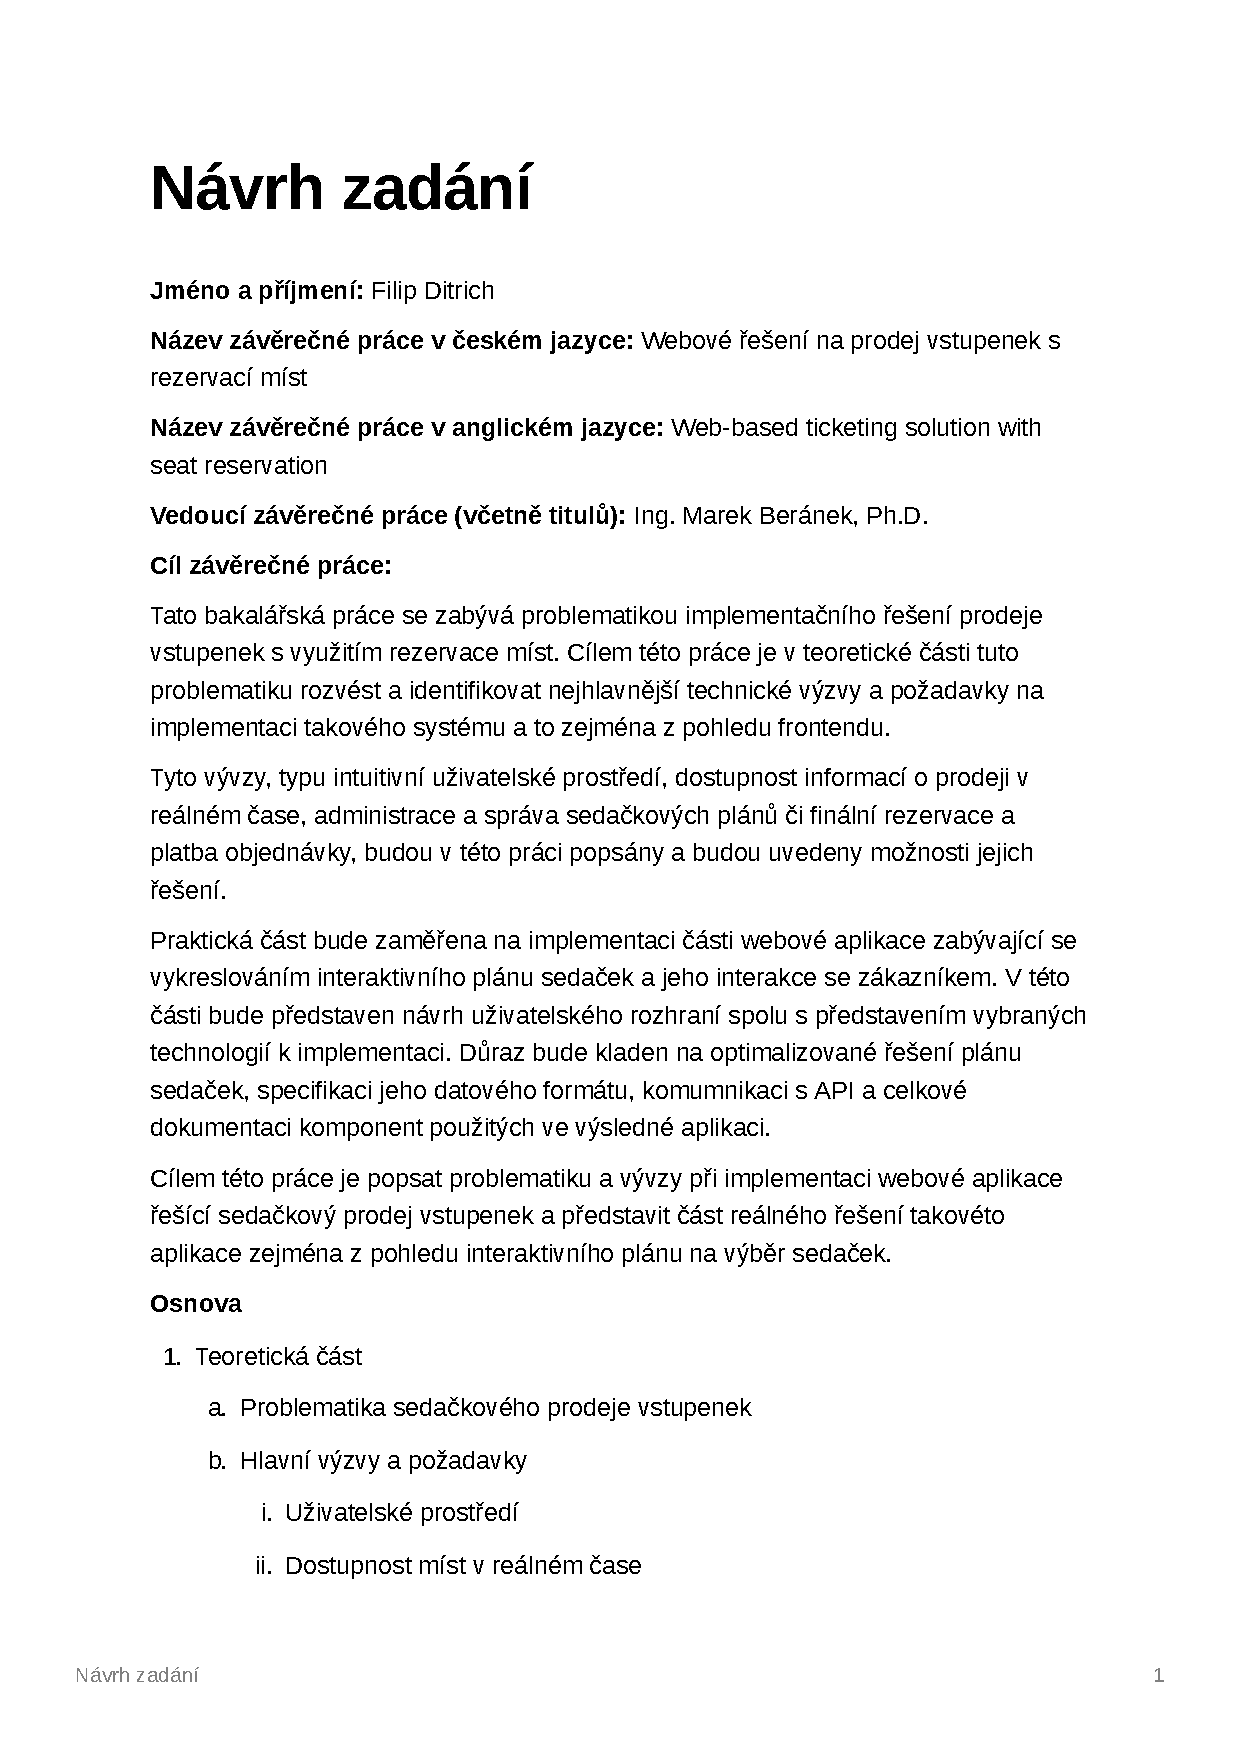
\includepdf[pages={1}]{\FIGDIR/navrh-zadani.pdf}
    \includepdf[pages={2}]{\FIGDIR/navrh-zadani.pdf}
%%% čestné prohlášení
    %%%
%%%  ČESTNÉ PROHLÁŠENÍ
%%%
%%%  * soubor obsahující čestné prohlášení k bakalářské práci
%%%
%%%  ===========================================================================
\newpage
\pagestyle{empty}
\vspace*{\stretch{8}}

%%% nadpis
\noindent
{\large\bfseries Čestné prohlášení}\\

%%% text
\noindent
Prohlašuji, že jsem svou bakalářskou práci na~téma \textit{Webové řešení na prodej vstupenek s~rezervací míst} vypracoval samostatně pod~vedením vedoucího bakalářské práce a s~použitím výhradně odborné literatury a~dalších informačních zdrojů, které jsou v práci všechny citovány a~jsou také uvedeny v~seznamu použitých zdrojů.\\

\noindent
Jako autor této bakalářské práce dále prohlašuji, že v~souvislosti s~jejím vytvořením jsem neporušil autorská práva třetích osob a~jsem si plně vědom následků porušení ustanovení § 11 a následujících autorského zákona č.~121/2000~Sb.\\

\noindent
Dále prohlašuji, že odevzdaná tištěná verze bakalářské práce je shodná s~verzí, která byla odevzdána elektronicky.

%%% podpis - místo/den
\vspace{18mm}
\noindent
V \makebox[4cm]{\dotfill} dne \makebox[2.5cm]{\dotfill}
\hspace*{\fill}
\makebox[4cm]{\dotfill}

%%% podpis
\begin{flushright}
    \noindent
    Filip Ditrich
\end{flushright}

%%% poděkování
    %%%
%%%  PODĚKOVÁNÍ
%%%
%%%  * soubor obsahující poděkování za pomoc při vytvoření bakalářské práce
%%%
%%%  ===========================================================================
\newpage
\pagestyle{empty}
\vspace*{\stretch{8}}

%%% nadpis
\noindent
{\large\bfseries Poděkování}\\

%%% TODO: text
\noindent
Rád bych touto cestou srdečně poděkoval vedoucímu bakalářské práce Ing.~Markovi Beránkovi,~Ph.D.
za~čas věnovaný vedením této práce, za~příjemnou spolupráci a~za cenné poskytnuté rady a připomínky.

%%% první stránka
    %%%
%%%  PRVNÍ STRANA
%%%
%%%  * soubor obsahující první stranu bakalářské práce
%%%
%%%  ===========================================================================
\newpage
\pagestyle{plain}

%%% začátek stránkování
\setcounter{page}{6}

%%% nastavení speciálních okrajů
\newgeometry{textwidth=100mm, textheight=247mm, left=40.4mm, right=75mm}

%%% pozadí
\tikz[remember picture,overlay]
\node[opacity=1,inner sep=0pt] at (current page.center)
    {
\includegraphics[width=\paperwidth,height=\paperheight]{\FIGDIR/side-banner}};

\begin{center}

    %%% logo školy
    \centerline{\mbox{
\includegraphics[width=39.6mm]{\FIGDIR/uu-icon}}}

    \vfill

    %%% název práce v češtině
    \Large\textbf{Webové řešení na prodej vstupenek s~rezervací míst}

    \vspace{5mm}

    %%% název práce v angličtině
    \Large{Web-based ticketing solution with seat reservation}

    \vfill

    %%% logo školy
    \centerline{\mbox{
\includegraphics[width=45mm]{\FIGDIR/uu-logo}}}

\end{center}
\restoregeometry

%%% abstrakt
    %%%
%%%  ABSTRAKT
%%%
%%%  * soubor obsahující abstrakt bakalářské práce
%%%
%%%  ===========================================================================
\newpage
\pagestyle{plain}

%%% abstrakt česky
\vbox to 0.5\vsize{
    \setlength\parindent{0mm}
    \setlength\parskip{5mm}

    %%% nadpis
    {\large\bfseries TODO: Abstrakt}

    %%% TODO: text abstrakt až po dopsání práce (lol)
    \noindent
    Tato bakalářská práce se zaměřuje na vývoj frontendové části webové aplikace pro prodej vstupenek s rezervací míst. Cílem práce je vyvinout prototyp aplikace, která potenciálnímu zákazníkovi umožní zobrazit mapu míst, vybrat si preferované místo, přidat vstupenky do nákupního košíku a následně vytvořit objednávku.

    Teoretická část práce se zaměřuje na obecnou problematiku prodeje vstupenek a moderního řešení pomocí platforem a služeb poskytujících online prodej vstupenek s možností rezervací míst. Tato část dále analyzuje trh současných poskytovatelů a definuje nejhlavnější technické problémy, které mohou při vývoji takového systému vzniknout a to výhradně z pohledu frontendu.

    Praktická část práce definuje rozsah implementované aplikace, podrobně popisuje hlavní funkce, komponenty, datové modely i některé nezbytné backendové části. Kapitola o návrhu uživatelského rozhraní popisuje principy, vzory a osvědčené postupy návrhu uživatelského rozhraní v kontextu vyvíjené aplikace. Kapitola o vývoji frontendové části poté podrobně popisuje technologie, nástroje a knihovny použité při vývoji aplikace.


    \vss}

%%% abstrakt anglicky
\nobreak\vbox to 0.49\vsize{
    \setlength\parindent{0mm}
    \setlength\parskip{5mm}

    %%% nadpis
    {\large\bfseries TODO: Abstract}

    %%% TODO: text anglicky
    \noindent
    This bachelor thesis deals with the implementation of a ticketing solution using seat reservations. The aim of
    the theoretical part of the thesis is to elaborate this issue and identify the main technical challenges and requirements for the implementation
    of such a system, especially from the frontend perspective. These challenges, such as intuitive user interface, availability of information
    real-time sales information, administration and management of seating plans or final booking and payment of orders, will be discussed in this thesis
    will be described in this thesis and options for their solution will be presented. The practical part will focus on the implementation of the part of the web application dealing with
    rendering of the interactive seating plan and its interaction with the customer. In this part the user interface design will be presented
    together with an introduction of the selected technologies to be implemented. Emphasis will be placed on the optimized design of the seating plan, the specification of
    of its data format, communcation with the API and overall documentation of the components used in the resulting application. The aim of this work is to describe
    the issues and challenges in implementing a web application addressing seat ticketing and present part of a real solution for such a
    application especially from the perspective of an interactive seat selection plan.

    Keywords: interactive seating plan, seat reservations, tickets, web applications, JavaScript, React, SVG
    \vss}


%%% obsah
    \newpage
    \pagestyle{plain}
    \tableofcontents
%%% TODO: jednotlivé kapitoly
    %%%%% Úvod
%%%%% ------------------------------------------------------------
\chapter*{Úvod}
\addcontentsline{toc}{chapter}{Úvod}

%%% Sekce - Prodej vstupenek
%%%%% Wording: ✅
%%%%% Styling: ✅
%%%%% References: ✅
%%%%% Grammar: ✅
%%% --------------------------------------------------------------
\section*{Prodej vstupenek}
\addcontentsline{toc}{section}{Prodej vstupenek}
\label{sec:uvod-prodej-vstupenek}
Prodej vstupenek na kulturní a jiné různé události je důležitou součástí zábavního průmyslu, neboť poskytuje lidem přístup na koncerty, divadelní představení, sportovní či jiné události.
Prodej vstupenek umožňuje pořadatelům těchto akcí nejen kontrolovaný průběh akce, ale především generuje dostatečný finanční tok peněz před konáním jejich akce.
Tyto finance zpravidla potřebují pro zajištění všech potřebných prostředků pro uspořádání akce a pro pořadatele se tedy jedná o jeden z klíčových faktorů úspěchu konání akce.
Potřebují tedy pro zákazníky zajistit co nejsnadnější a nejpříjemnější možnost nákupu vstupenek.

S nástupem moderních technologií se online prodej vstupenek proměnil v atraktivní a preferovaný způsob jejich nákupu, jelikož zákazníkům umožňuje snadný, pohodlný, a hlavně rychlý způsob platby, aniž by se museli kamkoliv fyzicky dostavit.
Tento nový moderní způsob prodeje vstupenek však nabízí výhody nejen zákazníkům, ale také pořadatelům akcí.
Systémy, které jsou na tomto způsobu prodeje vstupenek založeny, pořadatelům akcí umožňují bezproblémový prodej vstupenek, což vede k efektivnějšímu plánování a řízení akcí.
Tyto systémy pořadatelům také nabízejí cenné údaje o zákaznících, jejich preferencích a chování, které mohou využít při plánování marketingových strategií, cílených reklam či propagačních akcí za účelem zvýšení zapojení zákazníků a podpoření prodeje.

Jedním z nejvýznamnějších pokroků v této oblasti online řešení prodeje vstupenek bylo rozšíření o možnost rezervace míst v prostoru konání akce.
Toto řešení nově zákazníkům umožňuje zarezervovat si místo na dané události, což opět přináší několik výhod pro zákazníky, ale také pro pořadatele akcí.
Zákazníkům umožňuje rezervaci a výběr místa, které je pro ně nejvhodnější.
Pořadatelům akcí pak rezervace míst umožňuje předem plánovat kapacitu dané akce a také zjistit, jaké místo je pro zákazníky nejvíce preferované.
Dále také značně snižuje počet možných podvodů se vstupenkami, jelikož kapacita je jasně dána počtem míst k sezení a nelze ji snadno překročit.

Webová řešení prodeje vstupenek s rezervací míst se v posledních letech stávají stále více oblíbenými a využívanými v různých odvětvích, včetně zábavního průmyslu, sportu či cestování, jak je mj.\ možné vidět na grafu na obrázku~\ref{fig:polaris-market-research} znázorňujícího průzkum trhu v oblasti poskytování online systémů prodeje vstupenek.

\begin{figure}[H]
    \centering
    \caption{Graf zobrazující podíl zemí na trhu poskytování online systémů prodeje vstupenek.}
    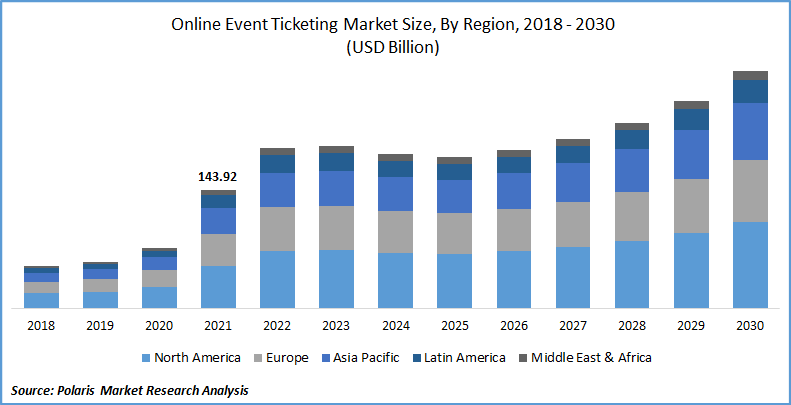
\includegraphics[width=\textwidth]{\FIGDIR/polaris-market-research}
    \source[\citeauthor{online_ticketing_polaris_market_research}]{}
    \label{fig:polaris-market-research}
\end{figure}

Avšak s rapidním vývojem v oblasti webových technologií je důležité sledovat a využívat nové trendy a technologie a přizpůsobovat jim takováto řešení, aby byla pro zákazníky stále atraktivní a relevantní.
Tato práce se proto zaměřuje na vývoj frontendové části webové aplikace prodeje vstupenek s rezervací míst, která bude využívat moderní webové technologie a nástroje, které jsou v současné době nejvíce využívané a oblíbené.
\pagebreak

%%% Sekce - Cíle práce
%%%%% Wording: ✅
%%%%% Styling: ✅
%%%%% References: ✅
%%%%% Grammar: ✅
%%% --------------------------------------------------------------
\section*{Cíle práce}
\addcontentsline{toc}{section}{Cíle práce}
\label{sec:uvod-cile-prace}
Cílem této práce je vyvinout prototyp responzivní webové aplikace nabízející prodej vstupenek s rezervací míst se zaměřením převážně na vývoj frontendové části.

Výsledkem této práce bude webová aplikace vyvinuta moderními webovými nástroji a technologiemi, která umožní potenciálním zákazníkům zobrazit mapu areálu nějaké akce či kulturní události, vybrat si jedno či více preferovaných míst, přidat si vstupenky do nákupního košíku a vytvořit tak objednávku.
Tato práce se bude zabývat vývojem takového webového řešení, ale pouze z pohledu frontendové části.
Ostatní funkčnosti, jako například backendový systém či administrační řešení, nebudou součástí této práce.

Nejprve bude ale pro vývoj třeba prozkoumat a analyzovat existující řešení prodeje vstupenek s rezervací míst, které jsou v současné době využívány.
Na základě identifikace klíčových částí takovýchto systémů budou následně vytvořeny dílčí uživatelské příběhy aplikace, které budou sloužit jako základ pro návrh uživatelského rozhraní.

Aby byla práce považována za úspěšně dokončenou, musí být splněny následující cíle:

\begin{itemize}
    \item Byly identifikovány klíčové prvky a funkčnosti webových řešení prodeje vstupenek s rezervací míst.
    \item Byl vytvořen návrh uživatelského rozhraní aplikace na základě definovaných uživatelských příběhů.
    \item Byla vyvinuta responzivní webová aplikace prodeje vstupenek s rezervací míst.
    \item Byla aplikace nasazena do produkčního prostředí.
\end{itemize}

    %%%%% Kapitola 1 - Analýza trhu
%%%%% ------------------------------------------------------------
\chapter{Analýza trhu}
\label{chap:analyza-trhu}
TODO: průzkum poskytovatelů, seznam jejich funkčností, strategií, taktik, popis, výhody a nevýhody

%%% Sekce - Ticketmaster
%%% --------------------------------------------------------------
\section{Ticketmaster}
\label{sec:analyza-trhu-ticketmaster}
TODO: popis Ticketmasteru

%%% Sekce - GoOut
%%% --------------------------------------------------------------
\section{GoOut}
\label{sec:analyza-trhu-goout}
TODO: popis GoOutu

%%% Sekce - NFCtron
%%% --------------------------------------------------------------
\section{NFCtron}
\label{sec:analyza-trhu-nfctron}
TODO: popis NFCtronu

    %%%%% Kapitola 3 - Specifikace prototypu
%%%%% ------------------------------------------------------------
\chapter{Specifikace prototypu}
\label{ch:specifikace}

Praktická část pojednává o~vývoji prototypu frontendu webové aplikace pro prodej vstupenek s~důrazem na implementaci funkčnosti rezervace míst.
Nutno podotknout že výsledný prototyp nebude a ani není v plánu, aby byl plně funkční, nýbrž pouze ukazuje možnou implementaci konkrétních zvolených částí.

K implementaci prototypu je důležité předem vydefinovat jasnou specifikaci a požadavky na výsledný produkt.
Bez těchto specifkací by nebylo možné finální výsledek objektivně zhodnotit.
A právě tato kapitola se zabývá různými klíčovými funkcemi a součástmi webového řešení pro prodej vstupenek a zkoumá a podrobně popisuje každý aspekt, aby bylo možné jasně pochopit požadovaných výsledek.
Tyto specifikace a požadavky pozdějí poslouží jako základ pro návrh a implementaci prototypu a následně i pro objektivní zhodnocení finálního výsledku.

%%% Sekce - Interaktivní mapa
%%% --------------------------------------------------------------
\section{Interaktivní mapa}
\label{sec:specifikace-interaktivni-mapa}
Vizualizace a celkové zobrazení interaktivní mapy sedaček místa konání akce je jednou z nejdůlěžitějších částí řešení webové aplikace na prodej vstupenek s rezervací míst.
Tato podkapitola se zabývá nejhlavnějšími aspekty vizualizace mapy sedaček, jako je celkové rozvržení a struktura, barevné kódování prvků na mapě, ovládání mapy, zobrazení dostupných informací o zvoleném místě a také důležitost dostupnosti dat v~reálném čase.
V každé sekci budou tyto aspekty podrobněji rozebrány, ukázány příklady z reálného světa a vysvětlena jejich důležitost.

%%% Podsekce - Rozložení a struktura
%%% --------------------------------------------------------------
\subsection{Rozložení a struktura}
\label{sec:specifikace-interaktivni-mapa-rozlozeni-a-struktura}
Pro docílení přehledného a uživatelsky přívětivého zobrazení plánku sedaček je třeba zajistit správnou vizuální stukturu a ideální rozložení prvků na obrazovce.
Dobře uspořádané uživatelské rozhraní pomáhá zákazníkům lépe se v mapě orientovat a vybrat tak preferovaná místa rychleji a snadněji.

Obrázek~\ref{fig:venue-map-visualization-layout-and-structure} zobrazuje příklad zasedacího pořádku portálu TICKETPORTAL v Divadle U Hasičů v Praze na Vinohradech.
V tomto zobrazení nalezneme indikaci hlediště, dostupných i nedostupných míst k sezení a číslování řad sedaček.
Toto zobrazení, ačkoliv poskytuje všechny důležité informace, není tolik uživatelsky přívětivé a atraktivní.
Například výběr správně kontrastního barevného zobrazení sedaček by celkovému zobrazení velmi prospělo.
Problematiku barevného kódování dále rozebírá následující sekce~\ref{sec:specifikace-interaktivni-mapa-barevne-kody}.

\begin{figure}[H]
    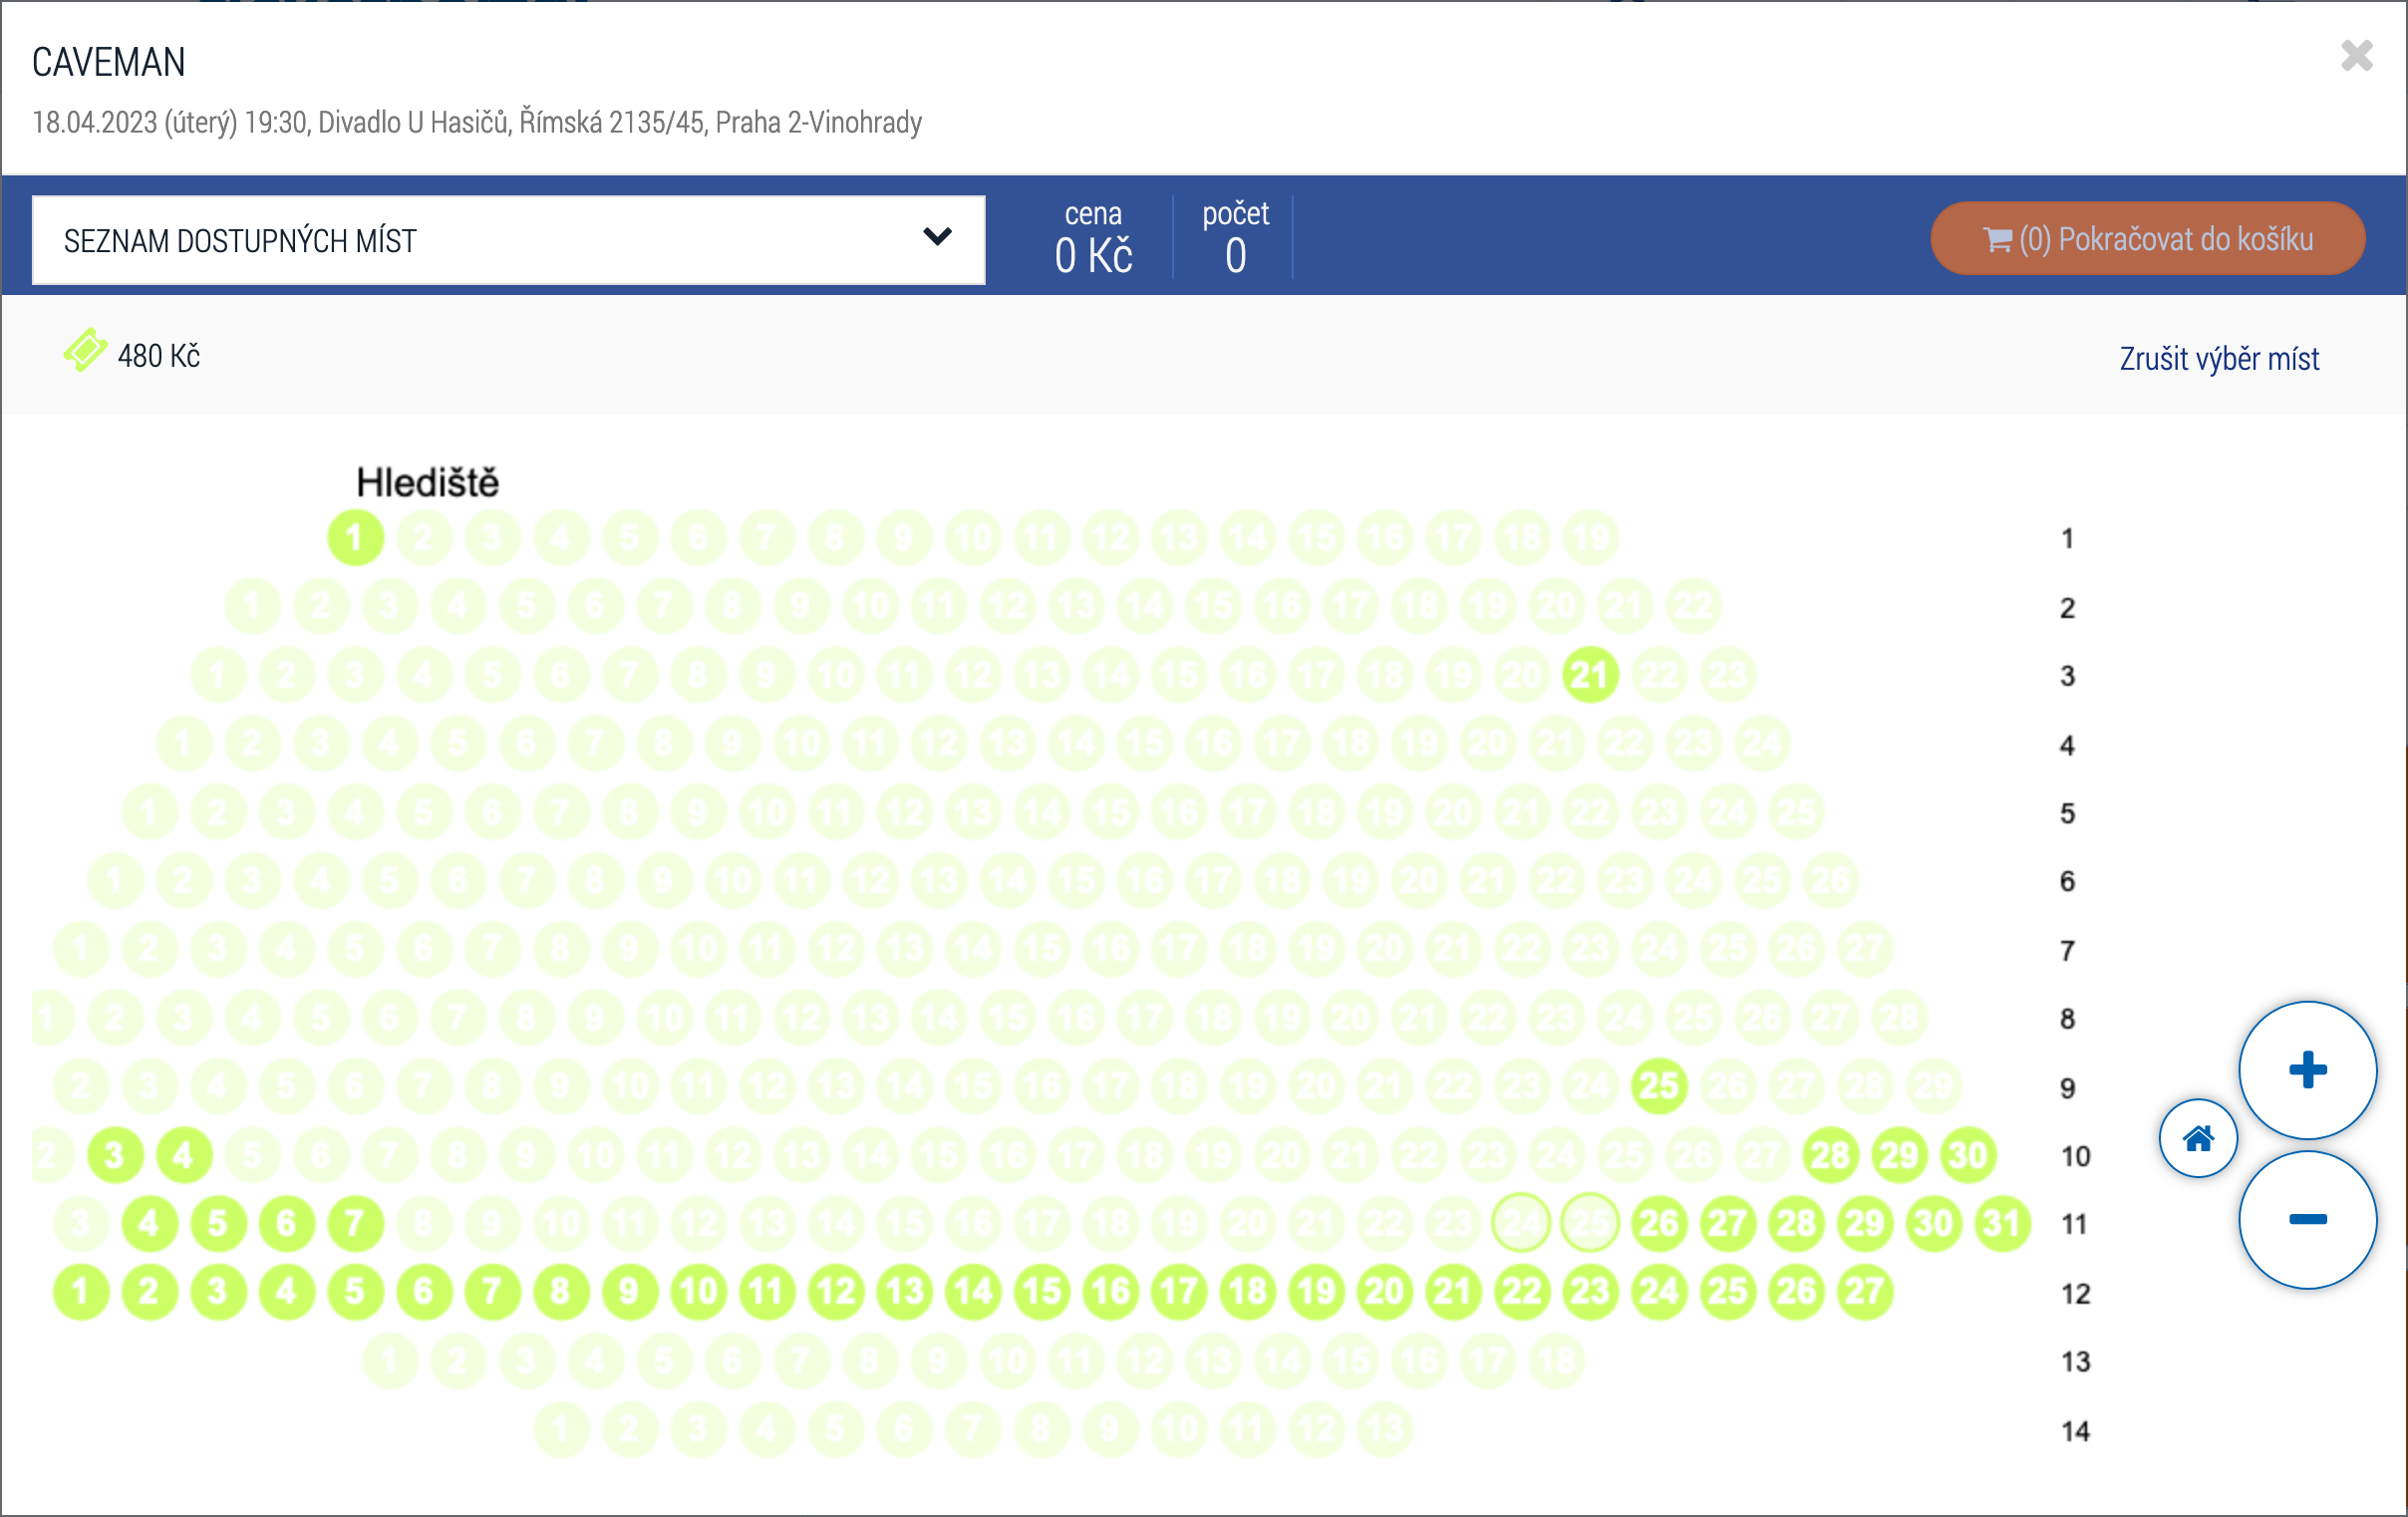
\includegraphics[width=\linewidth]{\FIGDIR/ticketportal-divadlo-u-hasicu}
    \centering
    \caption{Plánek sedaček v síti TICKETPORTAL}
    \label{fig:venue-map-visualization-layout-and-structure}
\end{figure}

Rozložení a struktura prvků na mapě by měly upřednostňovat uživatelskou přívětivost a snadnou navigaci, aby zákazníci mohli rychle najít a vybrat požadovaná místa.
Aby bylo tohoto dosaženo, měla by vizualizace mapy zahrnovat zřetelné sekce, jasné popisky a intuitivní uspořádání míst k sezení či případně i místa vymezená pro stání.

Nejdůležitější prvky, které by mapa měla obsahovat jsou:
\begin{enumerate}
    \item Místa k sezení - zvýrazněná místa k sezení, která jsou k dispozici pro výběr.
    \item Místa pro stání - místa, která jsou určena pro stání, mají větší kapacitu než místa k sezení a jsou také k dispozici pro výběr.
    \item Sektory - rozdělení větších plánku se sedačkami do jednotlivých sektorů seskupujích místa k sezení či stání.
    \item Hlediště - místo, kam budou hledět návštěvníci, důležité pro výběr místa s dobrým výhledem.
    \item Popisky - popisky pro zvýraznění významných míst, jako třeba řady nebo názvy sekcí.
    \item Značky pro zvýraznění dalších objektů - méně důležité, přesto informativní prvky na mapě jako třeba WC, bar, kavárna nebo zábradlí či sloupy.
\end{enumerate}

Tyto prvky by měli být jasně vizuálně definované a na mapě přehledně rozložené.
Záleží převážně o správnou definici a nakreslení prvků na mapě, což je úzce spojeno s administrací mapy a jejího nastavení.
Tu totiž musí někdo prvně vydefinovat a uložit do nějakého datového formátu.
Data si v tomto formátu poté vyžádá aplikace a na jejich základě mapu vykreslí uživateli v prohlížeči.
Touto problematikou se následně více zabývá sekce \ref{sec:implementace-mapa} v implementační části práce.

%%% Podsekce - Barevné kódování
%%% --------------------------------------------------------------
\subsection{Barevné kódování}
\label{sec:specifikace-interaktivni-mapa-barevne-kody}
Barevné kódování je dalším zásadním aspektem vizuálního zobrazení mapy místa konání, protože pomáhá uživatelům rychle identifikovat například kategorie míst, dostupnost a cenové úrovně sedadel.
Díky použití odlišných barev pro různé typy sedadel se zákazník v mapě může snadněji a rychleji orientovat.

Obrázek~\ref{fig:goout-color-codes} zobrazuje plánek míst sezení služby GoOut, který barevně odlišuje různé kategorie míst, dostupnost a cenové úrovně.

\begin{figure}[H]
    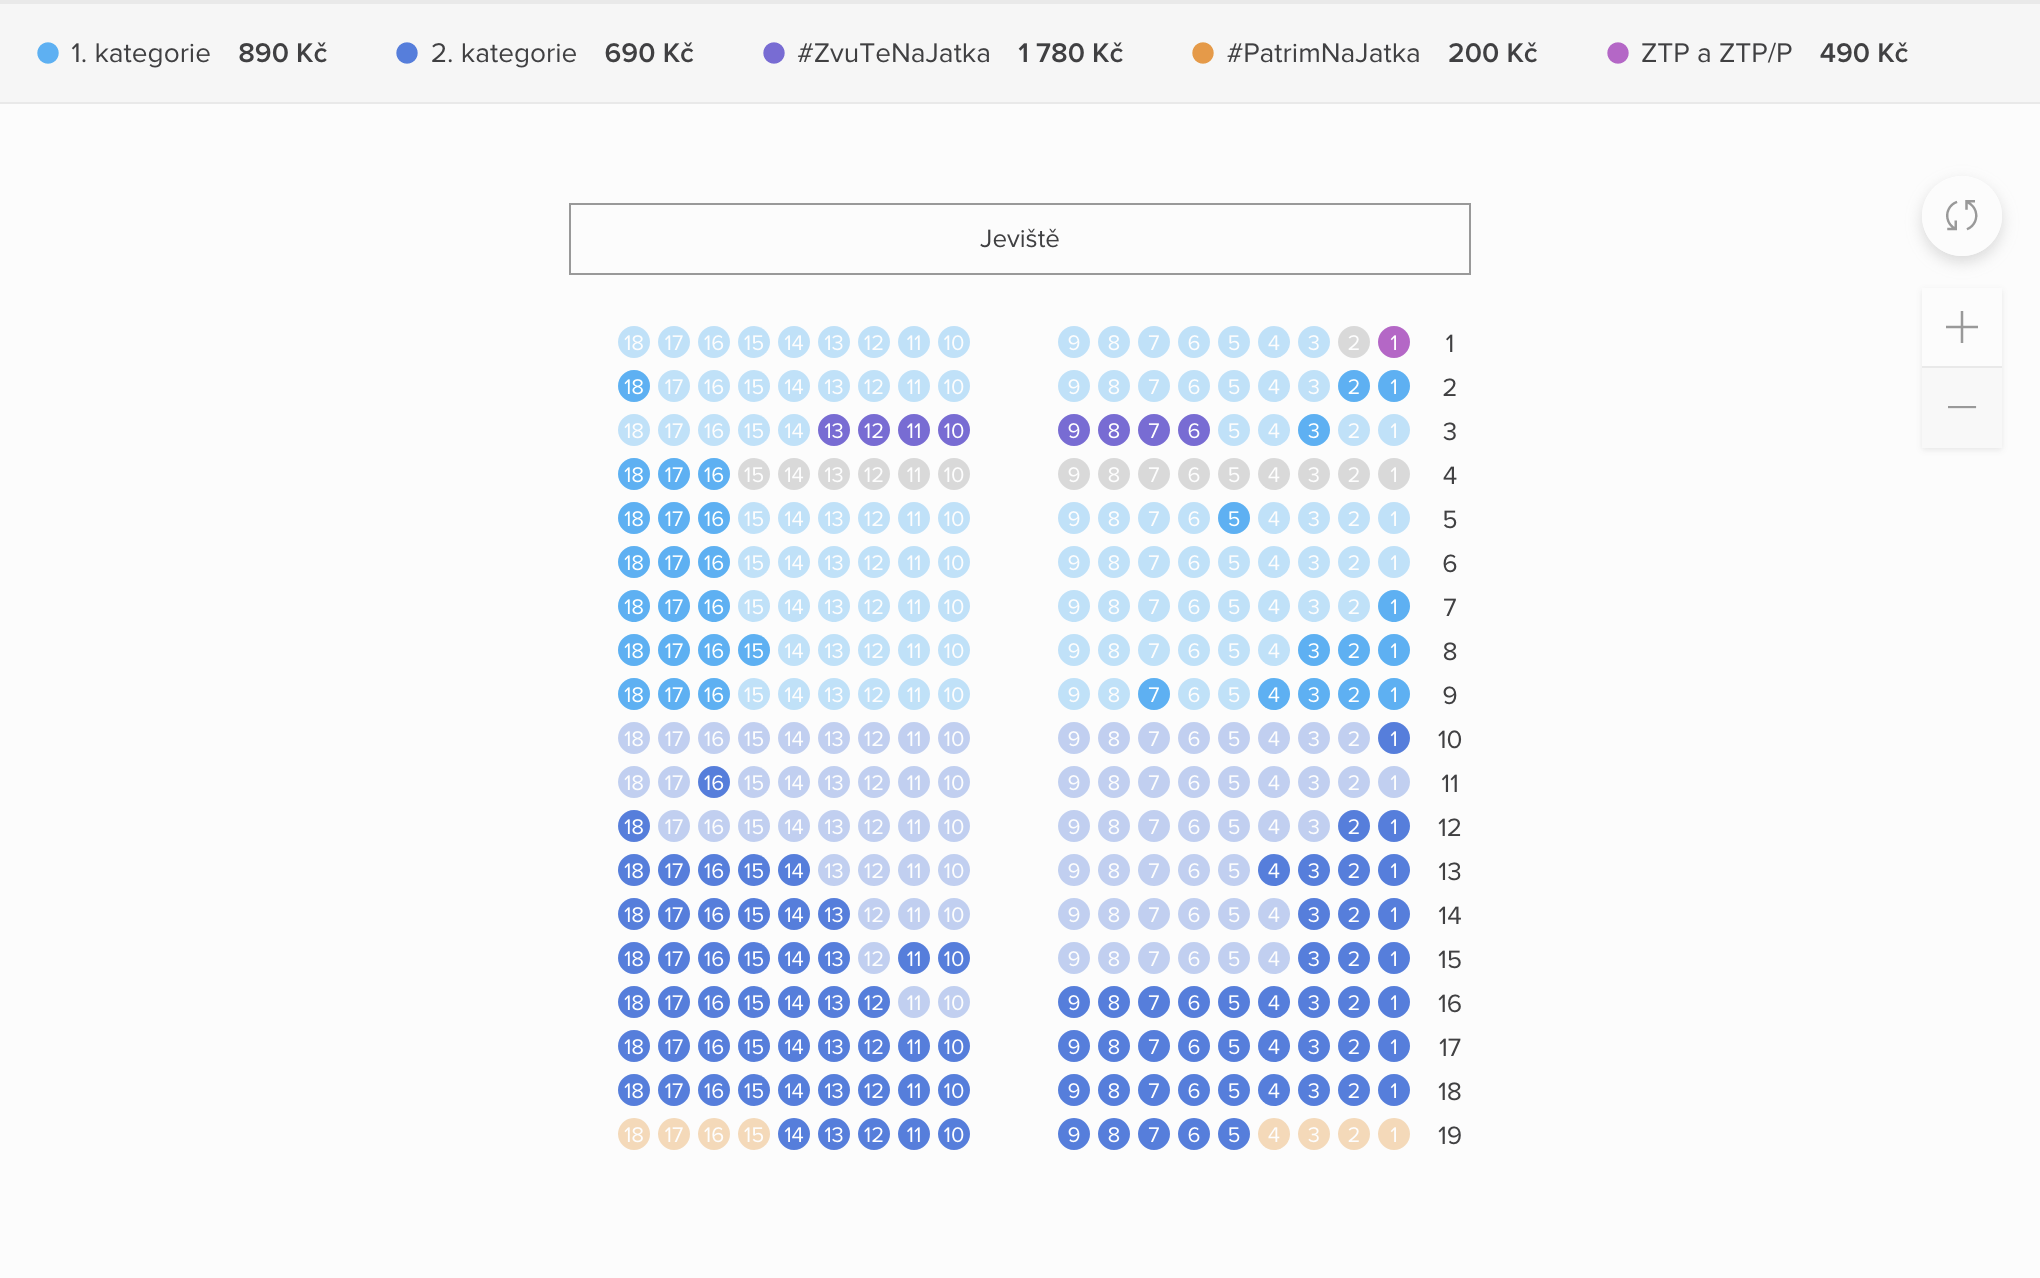
\includegraphics[width=\linewidth]{\FIGDIR/goout-color-codes}
    \centering
    \caption{Mapa barevně odlišených sedadel GoOut}
    \label{fig:goout-color-codes}
\end{figure}

Efektivní implementace barevného kódování vyžaduje použití snadno rozlišitelných barev, které vyhovují zákazníkům s různými zrakovými schopnostmi.
Zvolené barevné schéma by mělo zlepšit přehlednost a zvýšit uživatelský komfort tím, že zjednoduší proces výběru sedadel.
Pro zachování jednotného a přehledného zobrazení je výhodné předem definovat paletu barev, které budou moci být později použity pro různé prvky na mapě.
Užitím palety barev lze také jednodušeji udržet jednotnout vizuální identitu mapy a lze také předcházet zobrazenímu nekontrastních barevných kombinací, například textu na barevném podkladu.

%%% Podsekce - Ovládání mapy
%%% --------------------------------------------------------------
\subsection{Ovládání mapy}
\label{sec:specifikace-interaktivni-mapa-ovladani}
Ovládání zobrazení mapy je důležitou částí implementace, jelikož dodává větší interaktivnost tím, že umožňuje například pohyb kamery mapy po ose \em{x} a \em{y}, rotaci či přiblížení a oddálení.
Tyto funkce zákazníkovi umožňují podrobněji prozkoumat celou mapu místa a zároveň zobrazit více informací na jednom zobrazení.
Díky těmto funkcím získá zákazník také lepší přehled o celkovém rozpoložení míst v areálu.
Takovéto funkce jsou esenciální u zobrazení map větších areálů jako jsou například arény či stadiony.
Tyto mapy jsou totiž většinou ještě rozděleny do sektorů, které seskupují místa k sezení či stání.
Použitím funkce přiblížení a oddeálení lze také zobrazit různé úrovně detailu prvků na mapě v závislosti právě na hodnotě přiblížení.

Tento přístup například využívá síť \foreign{Ticketmaster}, který je možno vidět na obrázku~\ref{fig:ticketmaster-o2-zoom}, kde je demonstrována mapa sedadel s funkcí přiblížení a posunu a také s rozdělením na sektory.
Při oddálení mohou uživatelé zobrazit celkové rozložení místa konání rozdělené do sektorů.
Po přiblížení se zobrazí podrobnější zobrazení jednotlivých míst ve vybraném sektoru, což uživatelům umožňuje podrobně prozkoumat konkrétní oblasti areálu a vybrat požadované místo.

\begin{figure}[H]
    \centering
    \begin{subfigure}{0.45\textwidth}
        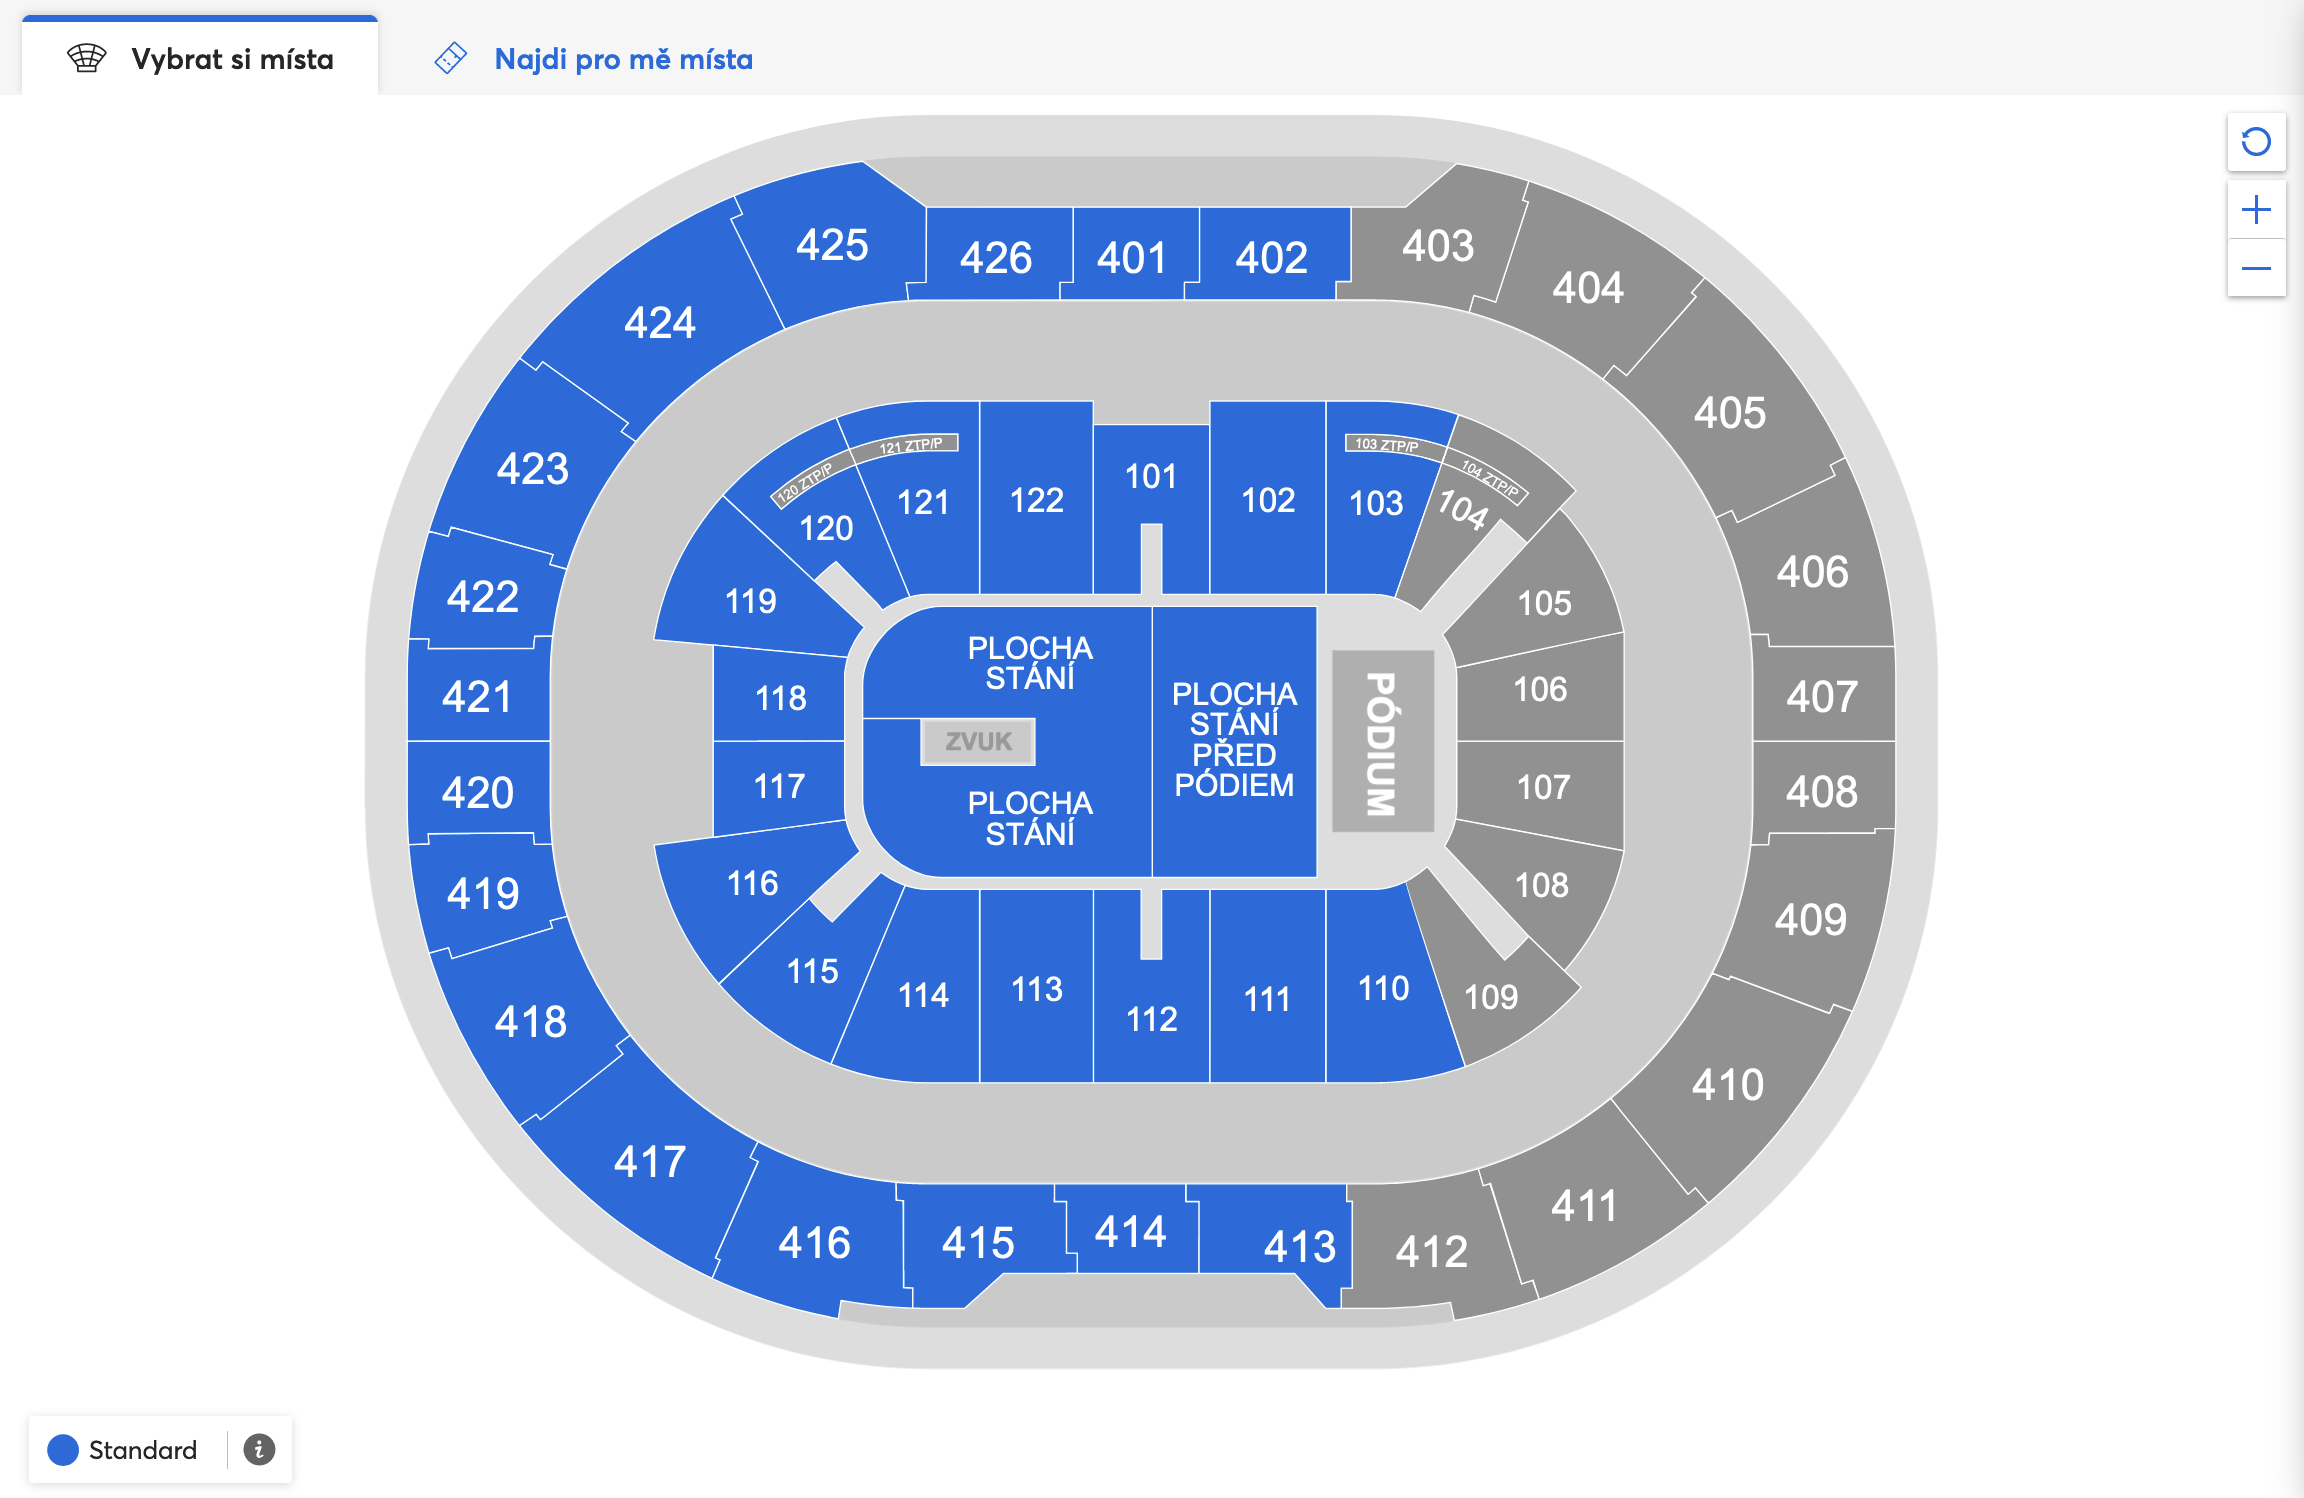
\includegraphics[width=\textwidth]{\FIGDIR/ticketmaster-o2-zoom-out}
        \caption{Oddálený pohled}
        \label{fig:ticketmaster-o2-zoom-in}
    \end{subfigure}
    \hfill
    \begin{subfigure}{0.45\textwidth}
        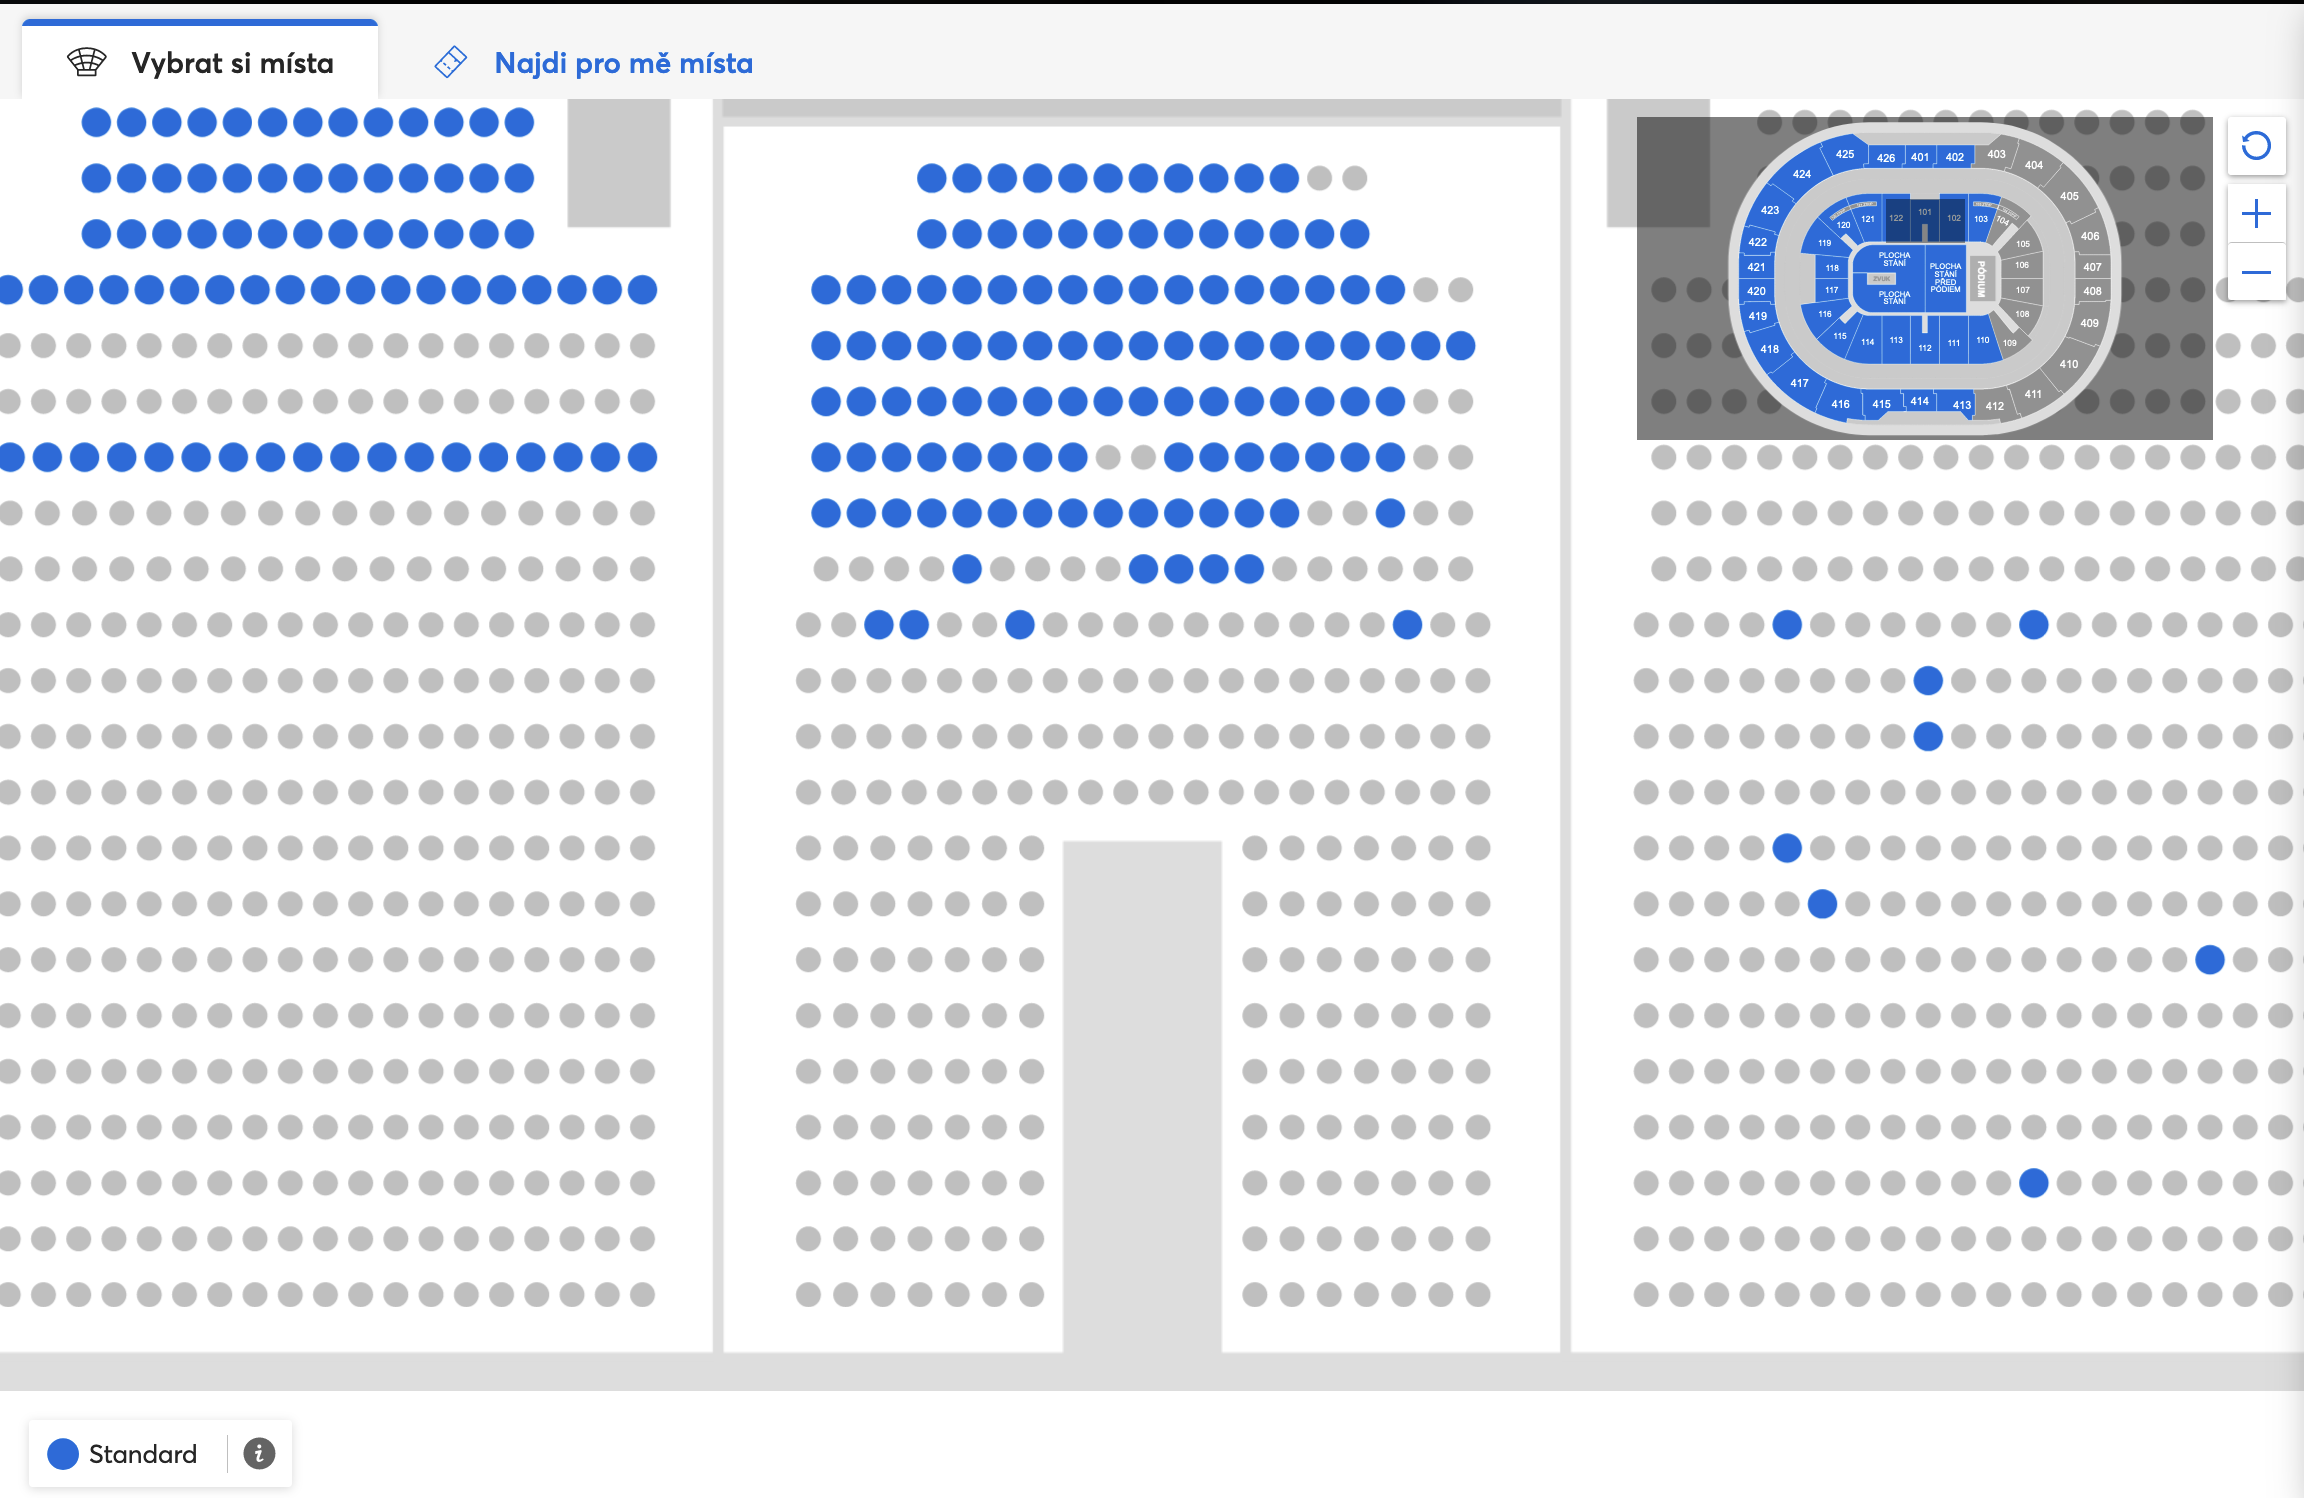
\includegraphics[width=\textwidth]{\FIGDIR/ticketmaster-o2-zoom-in}
        \caption{Přiblížený pohled}
        \label{fig:ticketmaster-o2-zoom-out}
    \end{subfigure}

    \caption{Různé pohledy mapy v síti Ticketmaster.}
    \label{fig:ticketmaster-o2-zoom}
\end{figure}

Při implementaci těchto funkčností je důležité myslet na přístupnost z pohledu koncových zařízení.
Například pro nedotyková zařízení tyto funkčnosti zajišťují ukazovací zařízení jako počítačové myši.
Na dotykových zařízeních jsou tyto funkčnosti docíleny pomocí dotykových gest \foreign{pinch} a \foreign{zoom} pro simulaci přiblížení a oddálení, gesta \foreign{rotate} pro rotaci a gesta \foreign{pan} pro pohyb na osách mapy.
Je tedy třeba zajistit podporu pro dotyková i nedotyková zařízení.
Často se k mapám zobrazuje i lišta s nástroji, které tyto funkčnosti ovládají.
V těchto lištách je také vhodné umístit tlačítko na vrácení zobrazení mapy do výchozího zobrazení.

%%% Podsekce - Stav a informace o sedadlech
%%% --------------------------------------------------------------
\subsection{Stav a informace o sedadlech}
\label{sec:specifikace-interaktivni-mapa-stav-a-informace-o-sedadlech}
Sedadla a ostatní místa k výběru o sobě nesou informace, které na mapě nemusejí být zřejmá a které zákazníkovi usnadňují výběr místa.
Tyto informace mohou být pro zákazníka zásadní, jelikož poskytují podrobnosti, jako je dostupnost, cena, přístupnost či další jiné popisy.
Díky těmto informacím se zákazník může lépe rozhodnout a vybrat si sedadlo, které nejlépe vyhovuje jeho preferncím a požadavkům.

Obrázek~\ref{fig:ticketmaster-o2-seat-info} zobrazuje mapu sedadel se stavem a informacemi o zvoleném sedadlu.
Uživatelé si mohou zobrazit  dostupnost, cenu a další důležité údaje o jednotlivých místech, což jim usnadňuje výběr preferovaných míst k sezení.

\begin{figure}[H]
    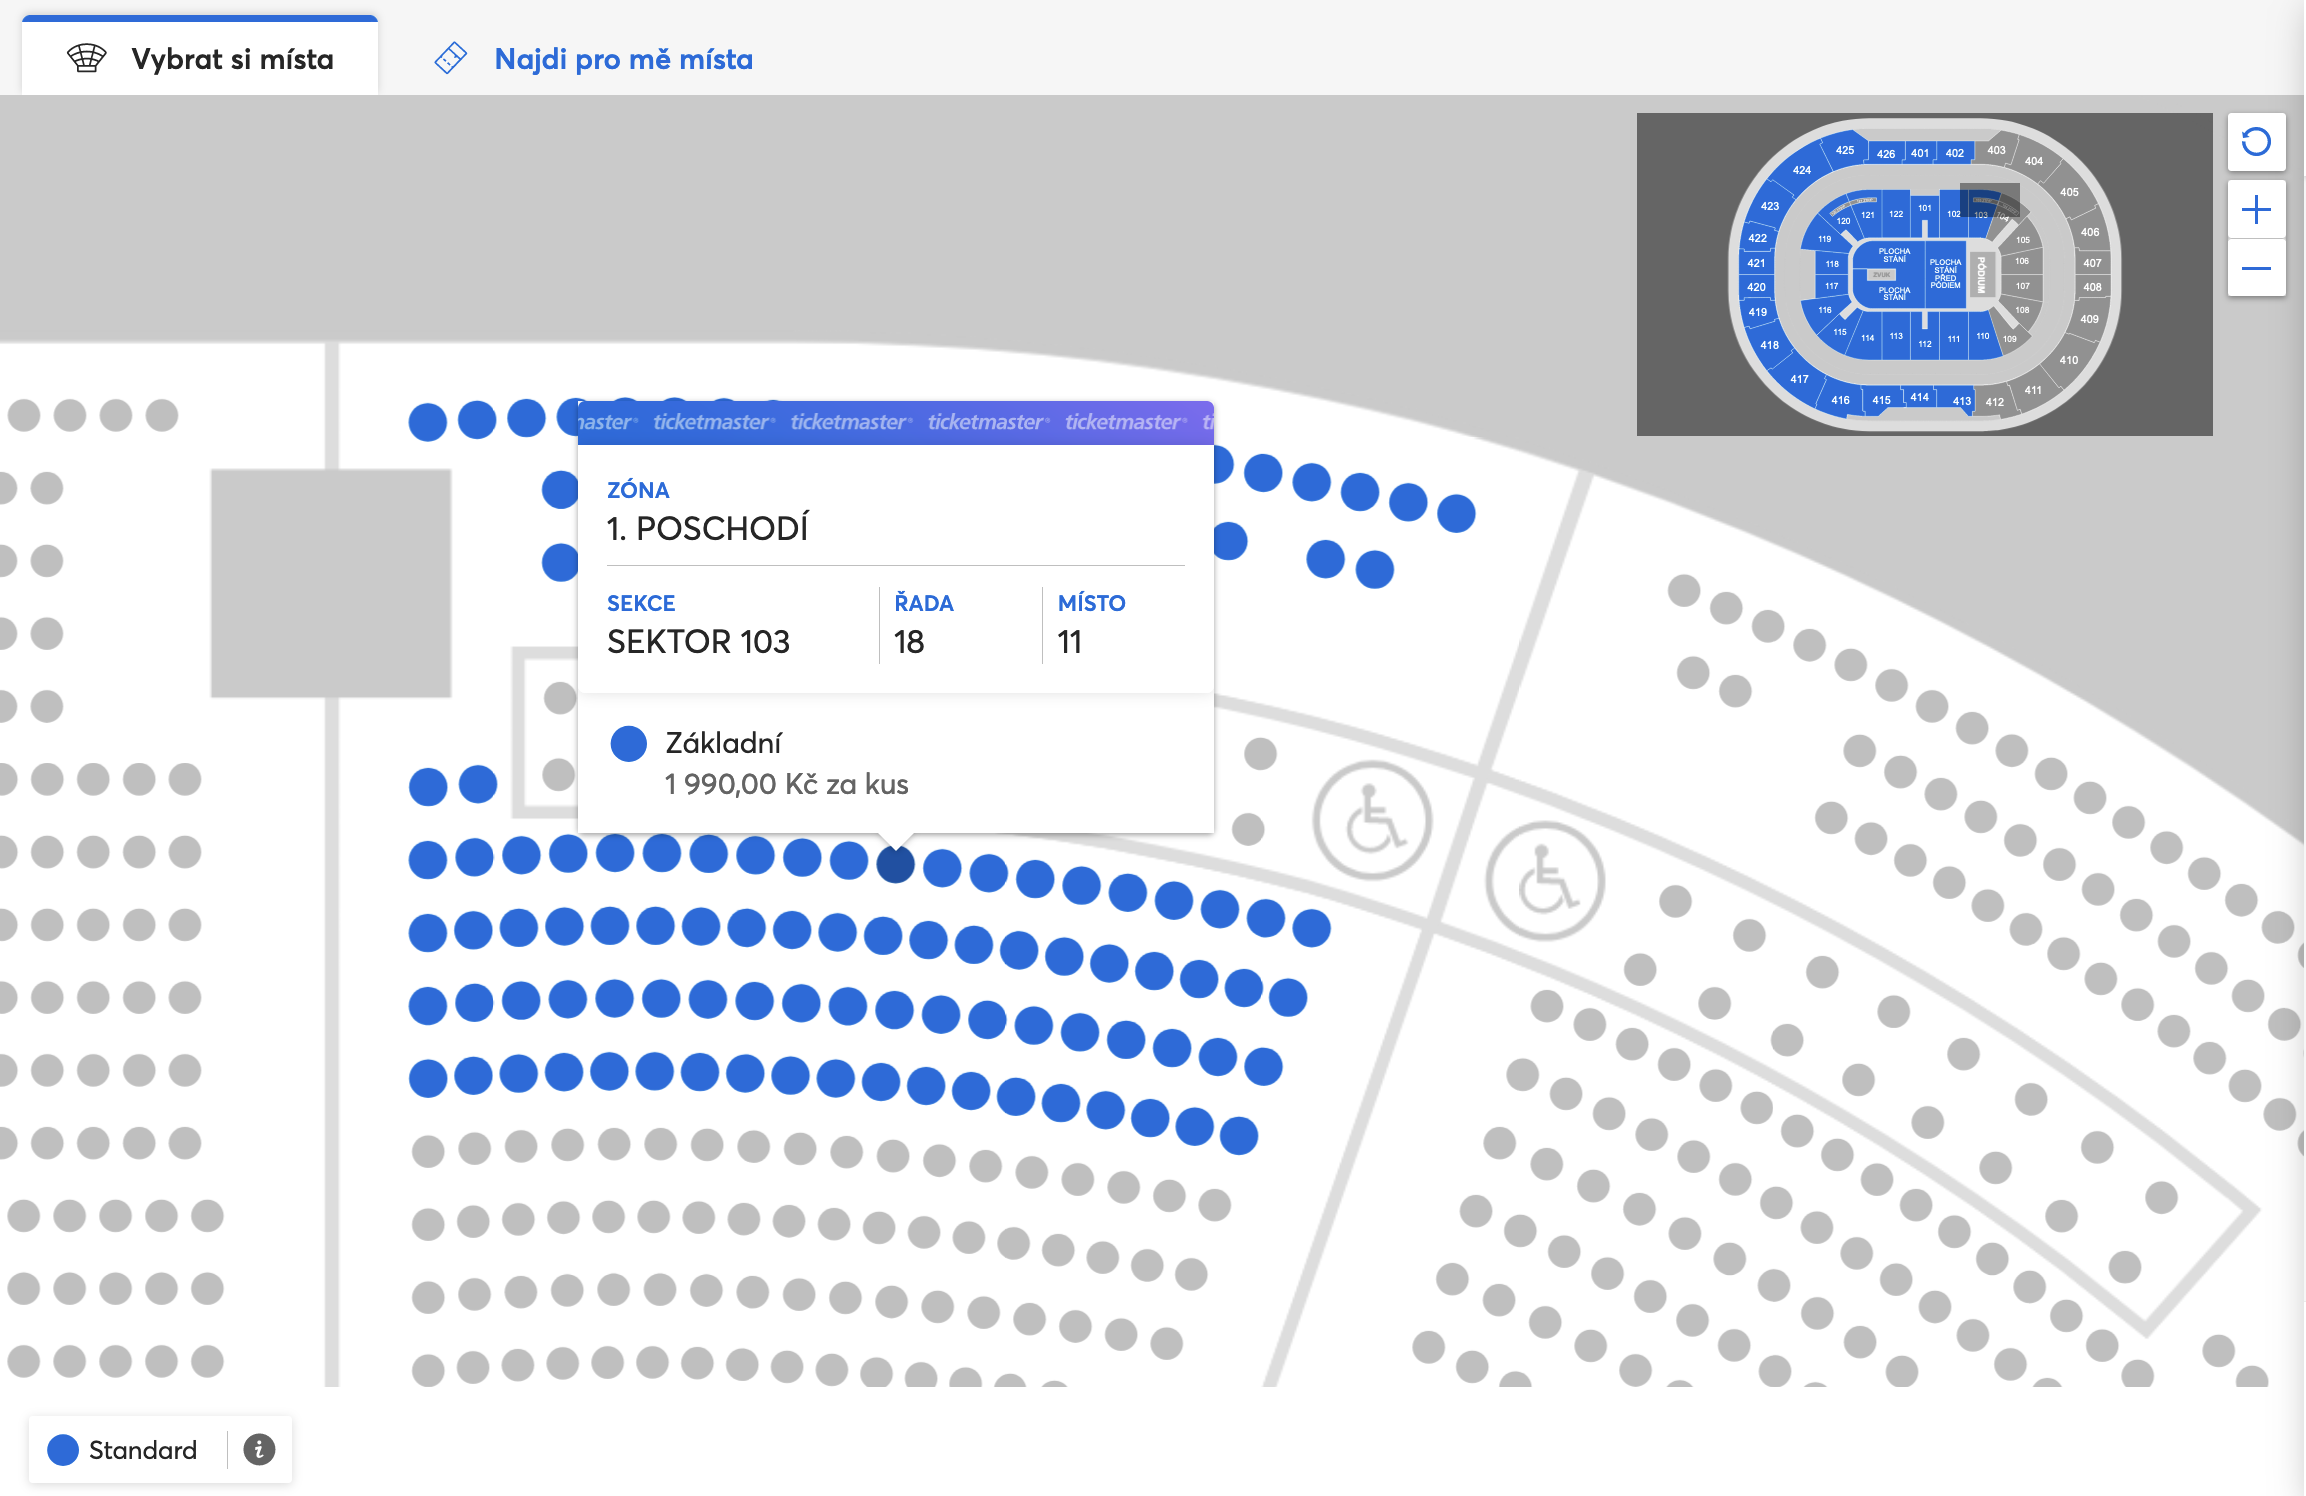
\includegraphics[width=\linewidth]{\FIGDIR/ticketmaster-o2-seat-info}
    \centering
    \caption{Informace o sedadle na mapě v síti Ticketmaster.}
    \label{fig:ticketmaster-o2-seat-info}
\end{figure}

Aby bylo možné efektivně implementovat informace o stavu sedadel, měla by být mapa míst jasná a srozumitelná a všechny důležité údaje by měly být snadno dostupné.
Jedním z běžných přístupů je použití vyskakovacích oken typu \foreign{popover} s informacemi, které se zobrazí  například po najetí myší.
Tato metoda však nemusí být vhodná pro mobilní a dotyková zařízení, kde takováto podobná gesta nefungují či fungují hodně omezeně.
Pro řešení tohoto problému lze použít alternativní přístup, a to například zobrazení informací o sedadle ve vyjíždějící spodní či boční liště po označení na sedadla.
Tím je zajištěno, že stav sedadla a informace o něm jsou přístupné uživatelům na všech zařízeních.

Toto okno či lišta by měla obsahovat ty nejdůležitější informace o zvoleném místě, jako:
\begin{enumerate}
    \item Řada a místo - číselné či alfanumerické označení řady a místa sedačky.
    \item Sektor - pokud je mapa rozdělena do sektorů, tak sektor, ve kterém se sedačka nachází.
    \item Cenu - cenu vstupenky odpovídající dané sedačce.
    \item Barevné označení - barevné označení sedačky, například dle její cenové kategorie.
    \item Stav sedačky - stav, ve kterém se sedačka vůči zákazníkovi nachází (obsazená, zvolená, nedostupná, \ldots).
    \item Další atributy - další informativní atributy, jako například informace o zhoršených podmínkách viditelnosti nebo vyhrazení místa pro osoby s postižením.
\end{enumerate}


%%% Podsekce - Data a jejich dostupnost
%%% --------------------------------------------------------------
\subsection{Data a jejich dostupnost}
\label{sec:specifikace-interaktivni-mapa-data-a-dostupnost}
Pro zobrazení a fungování aplikace je nezbytné mapu a celý její stav zkonstruovat pomocí reálných a aktualizovaných dat dostupných z backendového systému pomocí aplikačního rozhraní, označovaného jako \foreign{API}.
Tato data obsahují informace o vstupenkách a sedačkách jako například dostupnost, cena, umístění a další ostatní relevantní informace.
Struktura těchto dat by měla být jasně definovaná a dostupná ve formátu vyhovujícímu užití aplikace.

Areály s velkým množství sedaček mohou být problematické a to převážně z pohledu objemu přenášených dat mezi klientem a API.
Je důležité myslet na implementaci inteligentního datového přenosu, který zajistí komunikaci a přenos pouze nezbytných dat.
Díky menšímu objemu přenášených dat se pak zdá aplikace rychlejší a responzivnější.

Dalším aspektem práce s daty v takovéto aplikaci je aktualizace dat o dostupnosti.
Tato funkčnost zajišťuje zákazníkovi zobrazení aktuálních informací o sedačkách či vstupenkách a snižuje tak například riziko konfliktu výběru již obsazené sedačky.
Průběžné aktualizace dat lze docílit technologiemi jako například \foreign{WebSockets} nebo částečnými aktualizacemi dotazovanými skrze API.
Tyto metody budou později rozebrány v implementační části práce.


%%% TODO: Sekce - Nákupní košík
%%% --------------------------------------------------------------
\section{Nákupní košík}
\label{sec:specifikace-nakupni-kosik}
Velmi důležitou součástí fungování celého systému je efektivní správa a vizualizace nákupního košíku.
Ta například zákazníkovi poskytuje přehledný souhrn položek, které si objednává, a umožňuje mu je případně upravit či odebrat.
Nicméně ale tím nejdůležitejším aspektem nákupního košíku jsou jaká data jsou v něm uchovány a jakým způsobem jsou zpracována.

Tato podkapitola se zabývá popisem hlavním funkčností a požadavků na nákupní košík, které jsou nezbytné pro jeho efektivní fungování v rámci webového řešení s využitím rezervace sedadel.

\begin{figure}[H]
    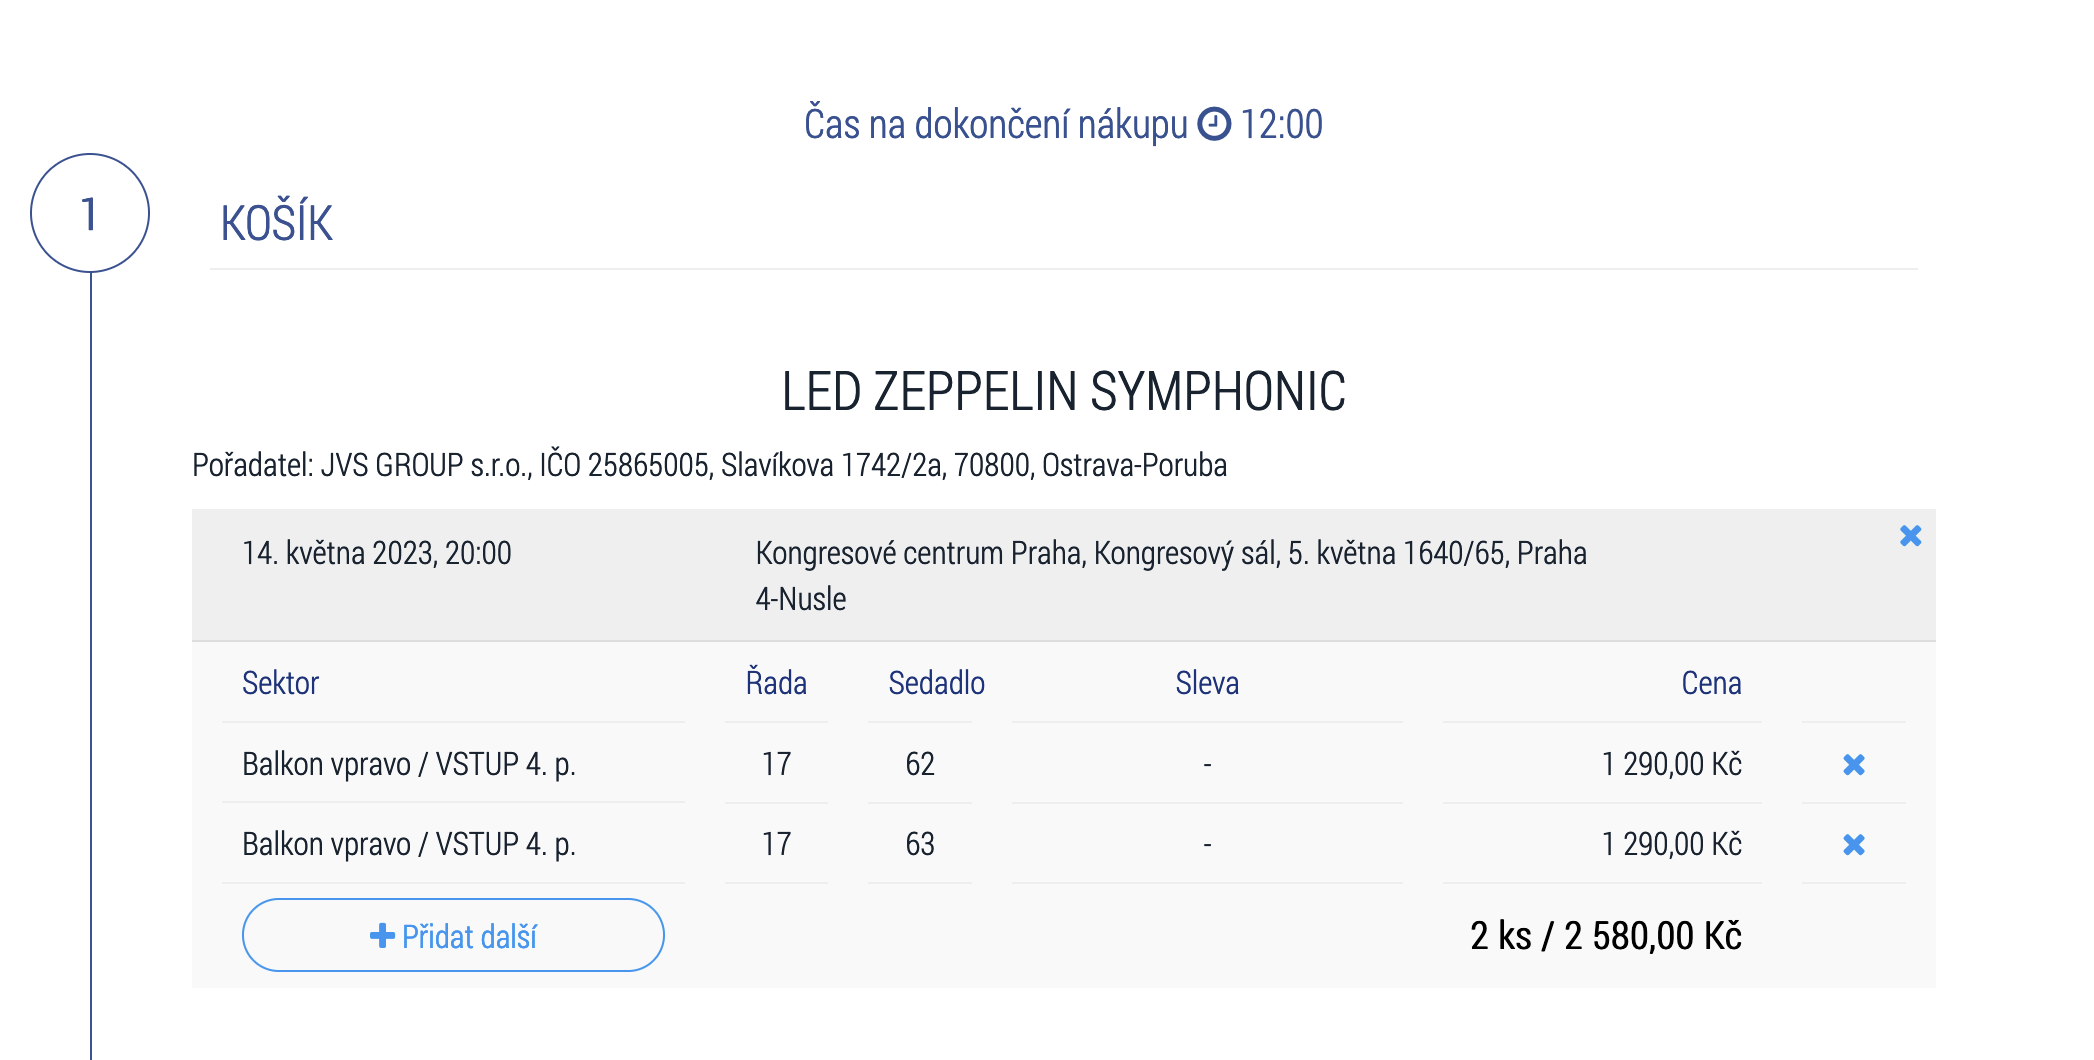
\includegraphics[width=\linewidth]{\FIGDIR/ticketportal-cart}
    \centering
    \caption{Obsah nákupního košíku na portálu Ticketportal.cz}
    \label{fig:ticketportal-cart}
\end{figure}

%%% TODO: Podsekce - Správa dat
%%% --------------------------------------------------------------
\subsection{Správa dat}
\label{sec:specifikace-nakupni-kosik-sprava}
Nákupní košík by z datové perspektivy měl být implementován jako objekt, který uchovává informace o všech vybraných sedačkách a vstupenkách.
Datová struktura a uchovávaná data uvnitř daného objektu o stavu nákupního košíku by měla být jasně definovaná a dostupná ve formátu vyhovujícímu užití aplikace.
Díky těmto datům by mělo být vždy možné zrekonstruovat stav nákupního košíku a to i v případě, že uživatel opustí stránku nebo zavře prohlížeč.

Touto problematikou se bude primárně zabývat kapitola~\ref{sec:implementace-kosik}, ve které bude podrobně popsána datavá struktura a finální funkčnost nákupního košíku.

%%% TODO: Podsekce - Přehled obsahu košíku
%%% --------------------------------------------------------------
\subsection{Přehled obsahu košíku}
\label{sec:specifikace-nakupni-kosik-prehled}
Pro zákazníka nákupní košík slouží primárně k přehlednému zobrazení všech vybraných položek, které budou tvořit jeho objednávku. V případně této webové aplikace se primárně jedná o vstupenky a zarezervované sedačky.

Zákazník by měl být schopen jednoduše zjistit, jaké položky si objednává a jaké mají parametry. Seznam všech těchto položek posléze tvoří celkový přehled nákupního košíku, který umožňuje zákazníkovi zkontrolovat jeho výběr a provést případné změny před dokončením objednávky.

\begin{figure}[H]
    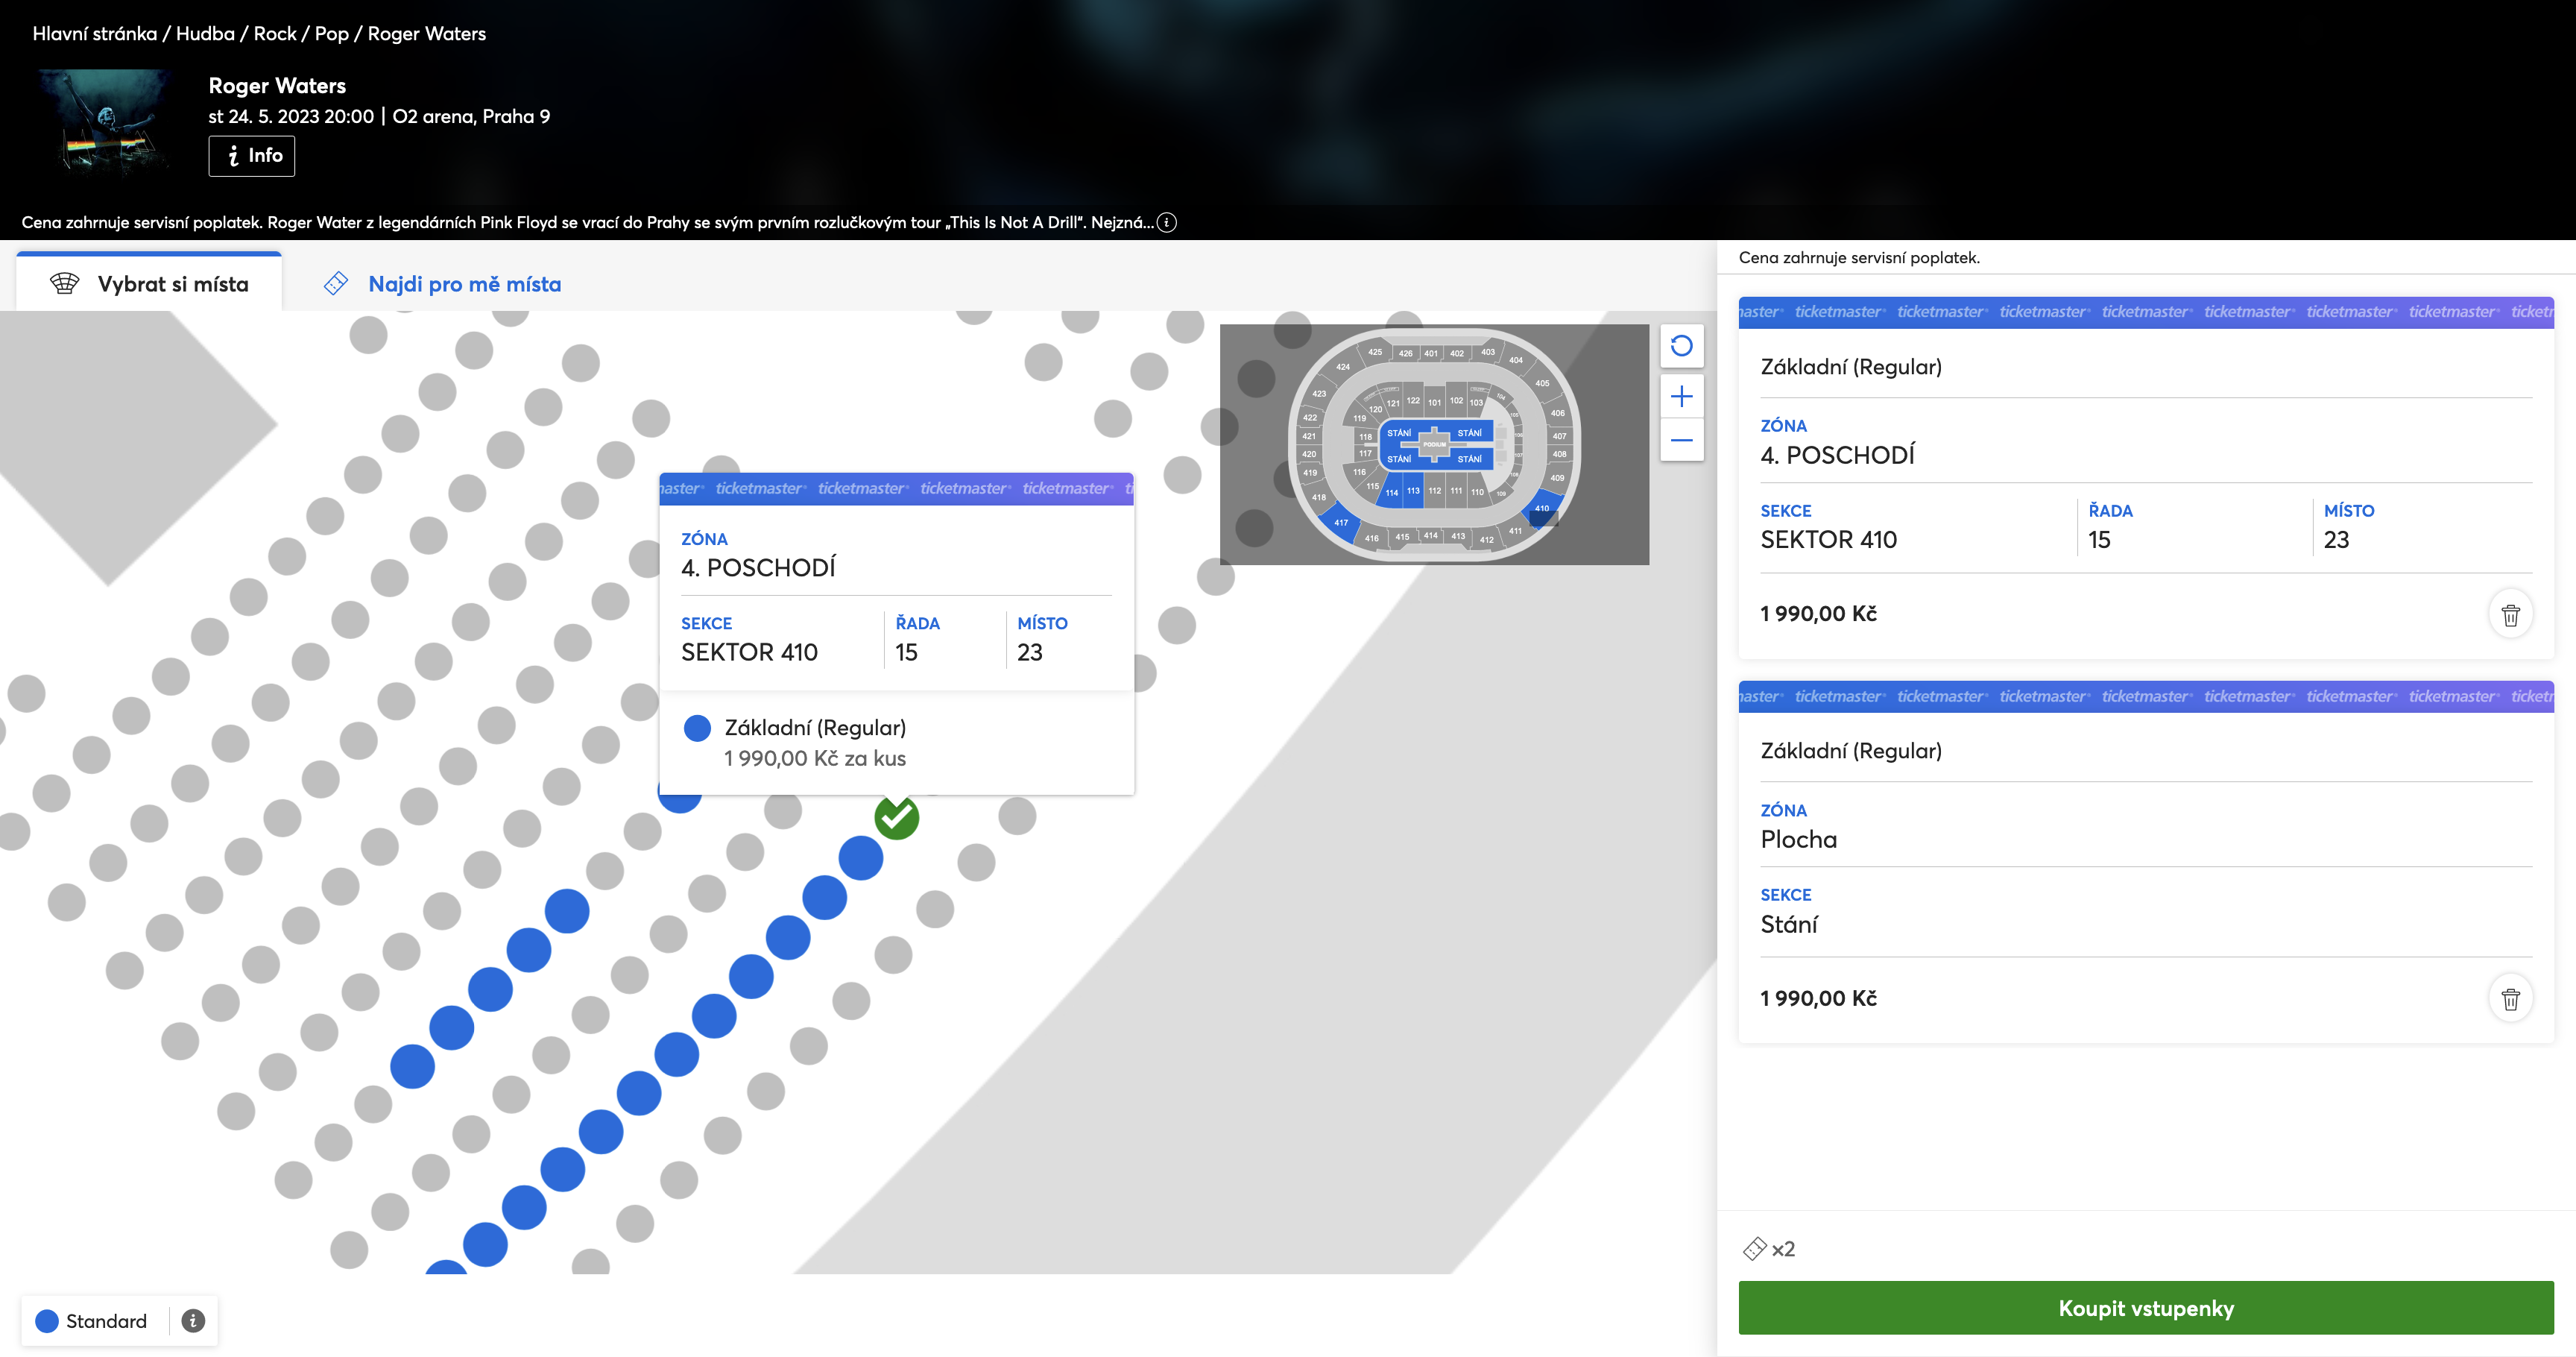
\includegraphics[width=\linewidth]{\FIGDIR/ticketmaster-cart-overview}
    \centering
    \caption{Nákupní košík na portálu Ticketmaster.com}
    \label{fig:ticketmaster-cart-overview}
\end{figure}

Nákupní košík by zároveň měl zobrazit přehled cen jednotlivých položek a celkovou cenu objednávky včetně všech daní a dalších případních poplatků. Tato funkcionalita zákazníkovi zajišťuje naprostou transparentnost v nabízených službách a umožňuje mu předem zkontrolovat celkovou cenu objednávky.

\begin{figure}[H]
    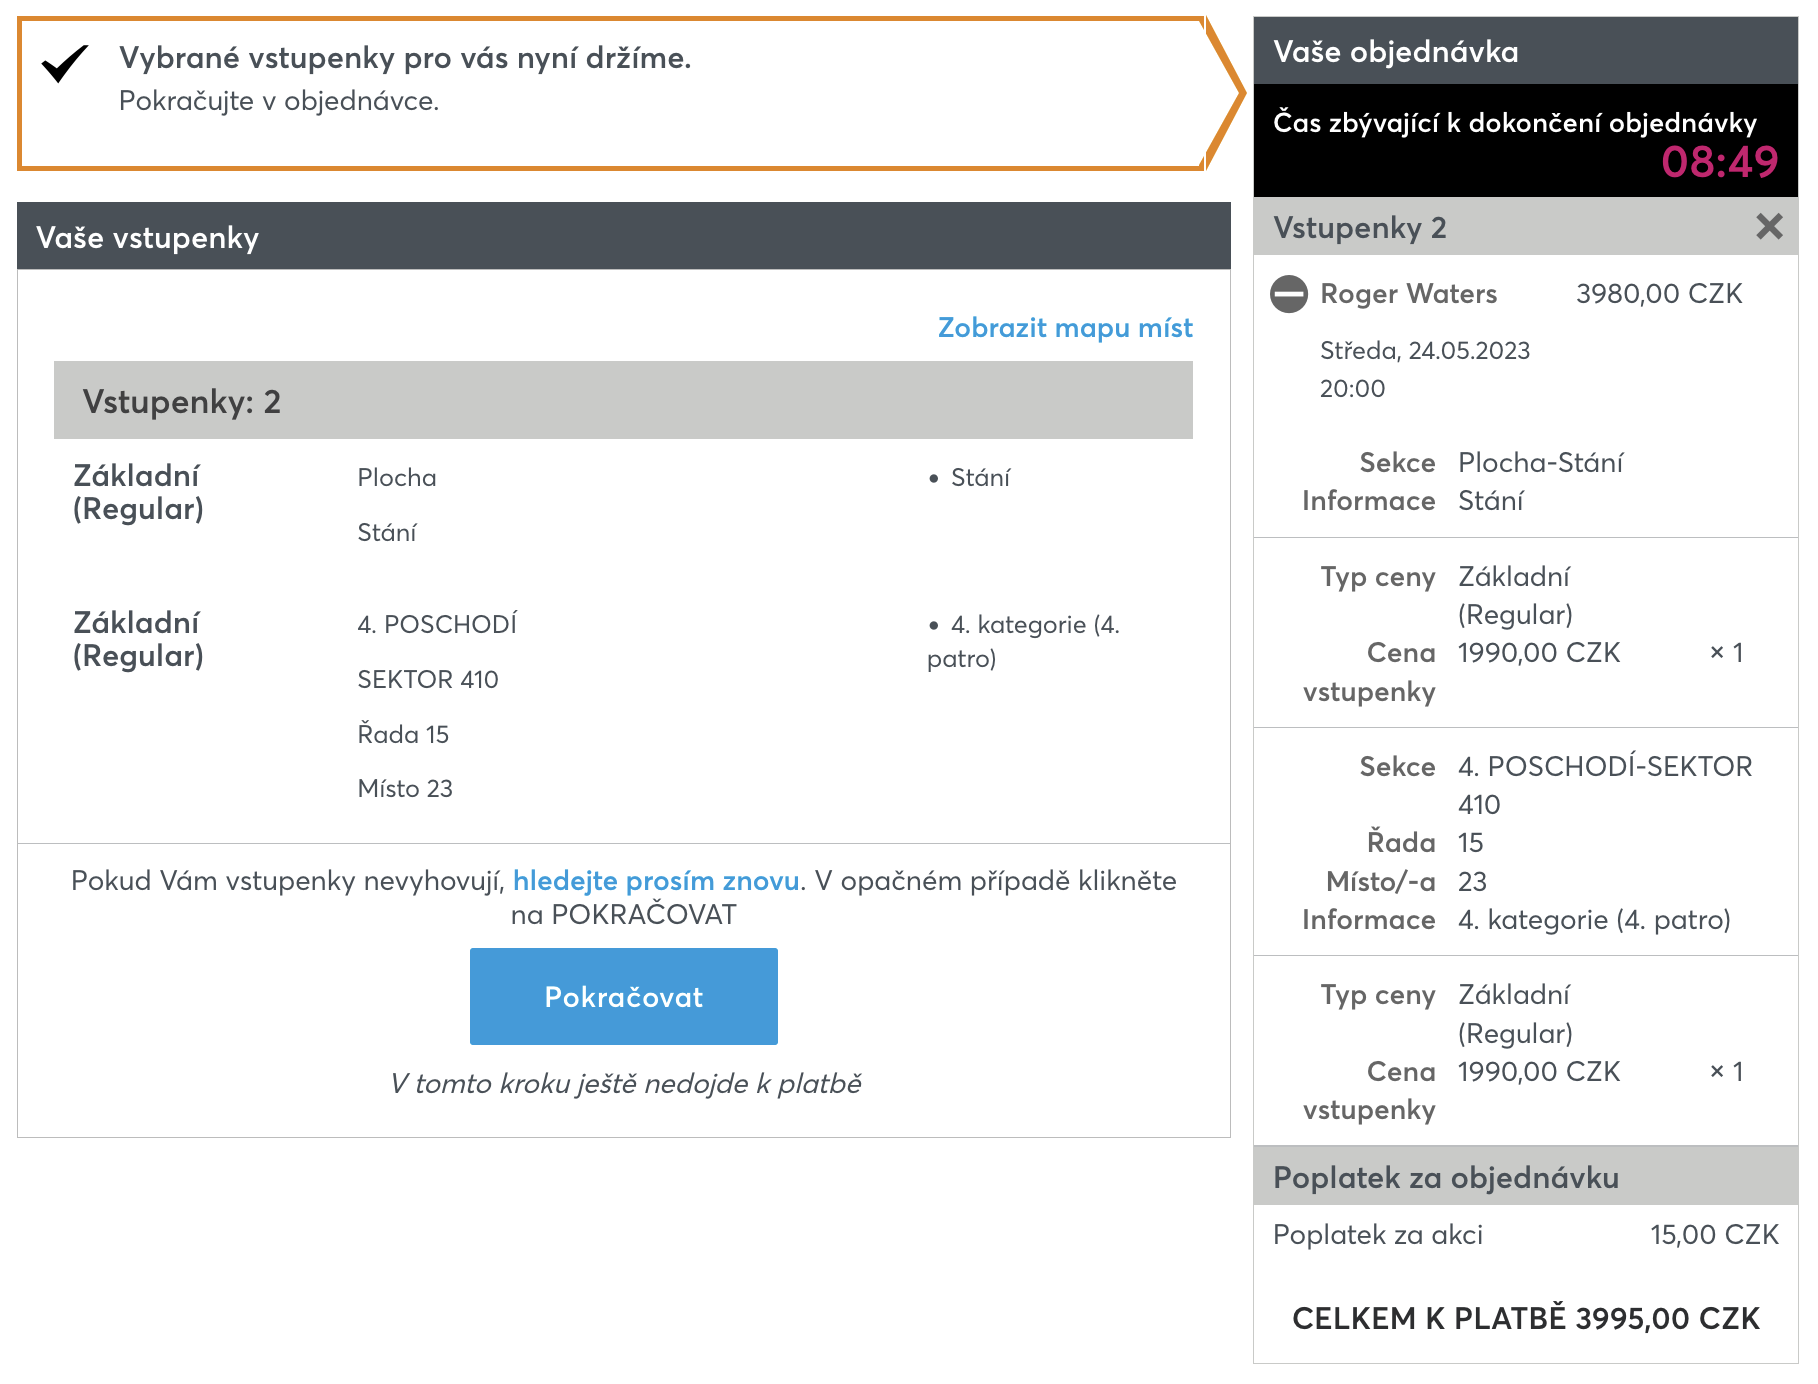
\includegraphics[width=\linewidth]{\FIGDIR/ticketmaster-cart-summary}
    \centering
    \caption{Souhrn objednávky na portálu Ticketmaster.com}
    \label{fig:ticketmaster-cart-summary}
\end{figure}


%%% TODO: Podsekce - Rezervace míst
%%% --------------------------------------------------------------
\subsection{Rezervace míst}
\label{sec:specifikace-nakupni-kosik-rezervace}
V rámci nákupního procesu si zákazník vybírá místa, které jsou dostupná a při jejich výběru se zákaznikovi přidají do nákupního košíku. Tato vybraná místa zákazníkem by se měla rezervovat, aby se předešlo nepříjemným situacím při dokončení objednávky, kdy zákazník zjistí, že jeho vybrané místo je již obsazené.

V případně aplikace, která se primárně zaměřuje na sedadlový prodej vstupenek je tato funkcionalita naprosto esenciální. Zákazník by měl mít možnost vybrat si místa, která jsou v danou chvíli dostupná a při jejich výběru by se měla pomocí rezervačnícho mechanismu v rámci vytvářené objednávky zákazníkovi zarezervovat a garantovat mu v případně dokonení objednávky jejich dostupnost.

Tento rezervační systém by měl dále implementovat funkčnost časového omezení rezervace, která zajistí uvolnění rezervovaných míst po uplynutí určitého časového limitu. Tato funkčnost je velmi důležitá pro zajištění dostupnosti míst pro všechny zákazníky a zabraňuje zarezervování sedadel, která by nebyla zakoupena například z důvodu opuštění nákupního procesu zákazníkem.

V rámci tohoto rezervačního mechanismu by také mělo být zákazníkovi jasně zobrazeno, že má určitý časový limit, ve rámci kterého musí svou objednávku dokončit, jinak se jeho rezervace uvolní a bude si muset místa vybrat znovu.

\begin{figure}[H]
    \centering
    \begin{subfigure}{0.3\textwidth}
        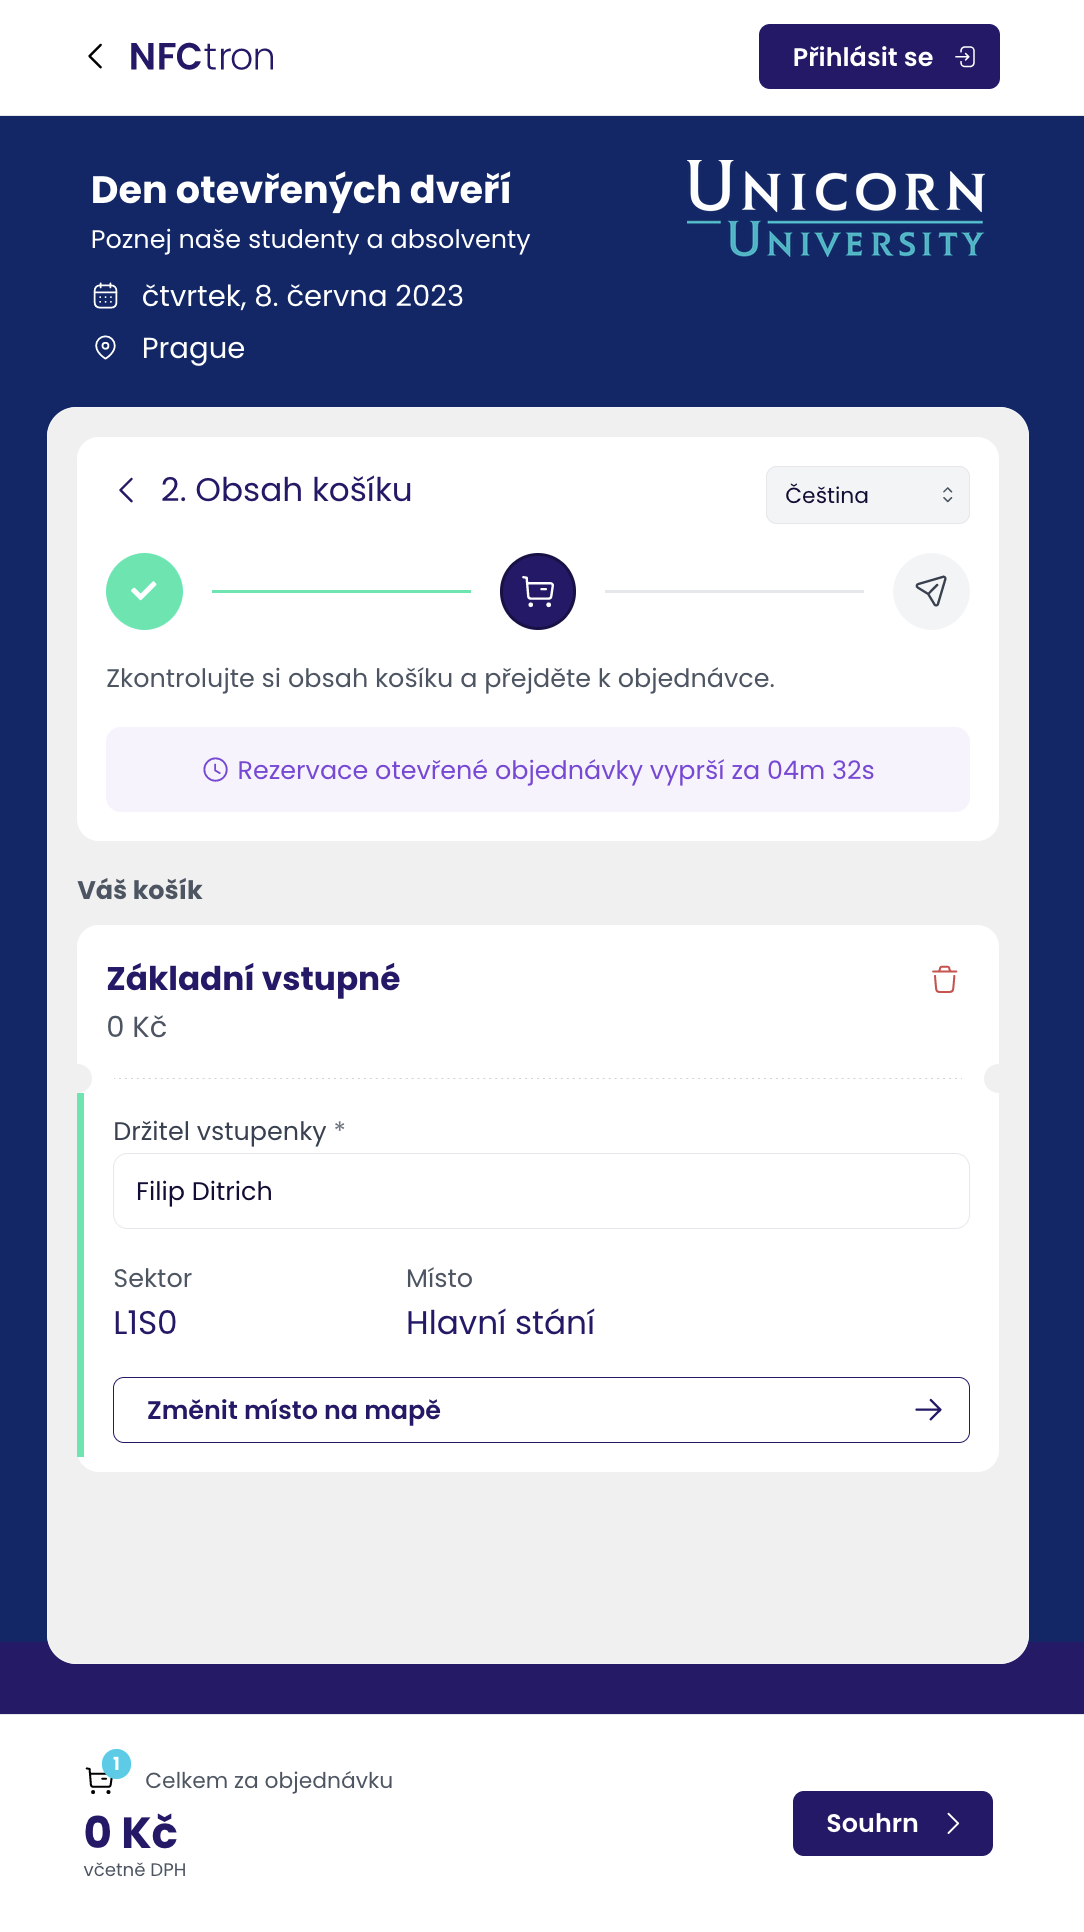
\includegraphics[width=\textwidth]{\FIGDIR/nfctron-tickets-reservation-pending}
        \caption{Běžící rezervace}
        \label{fig:nfctron-tickets-reservation-pending}
    \end{subfigure}
    \hfill
    \begin{subfigure}{0.3\textwidth}
        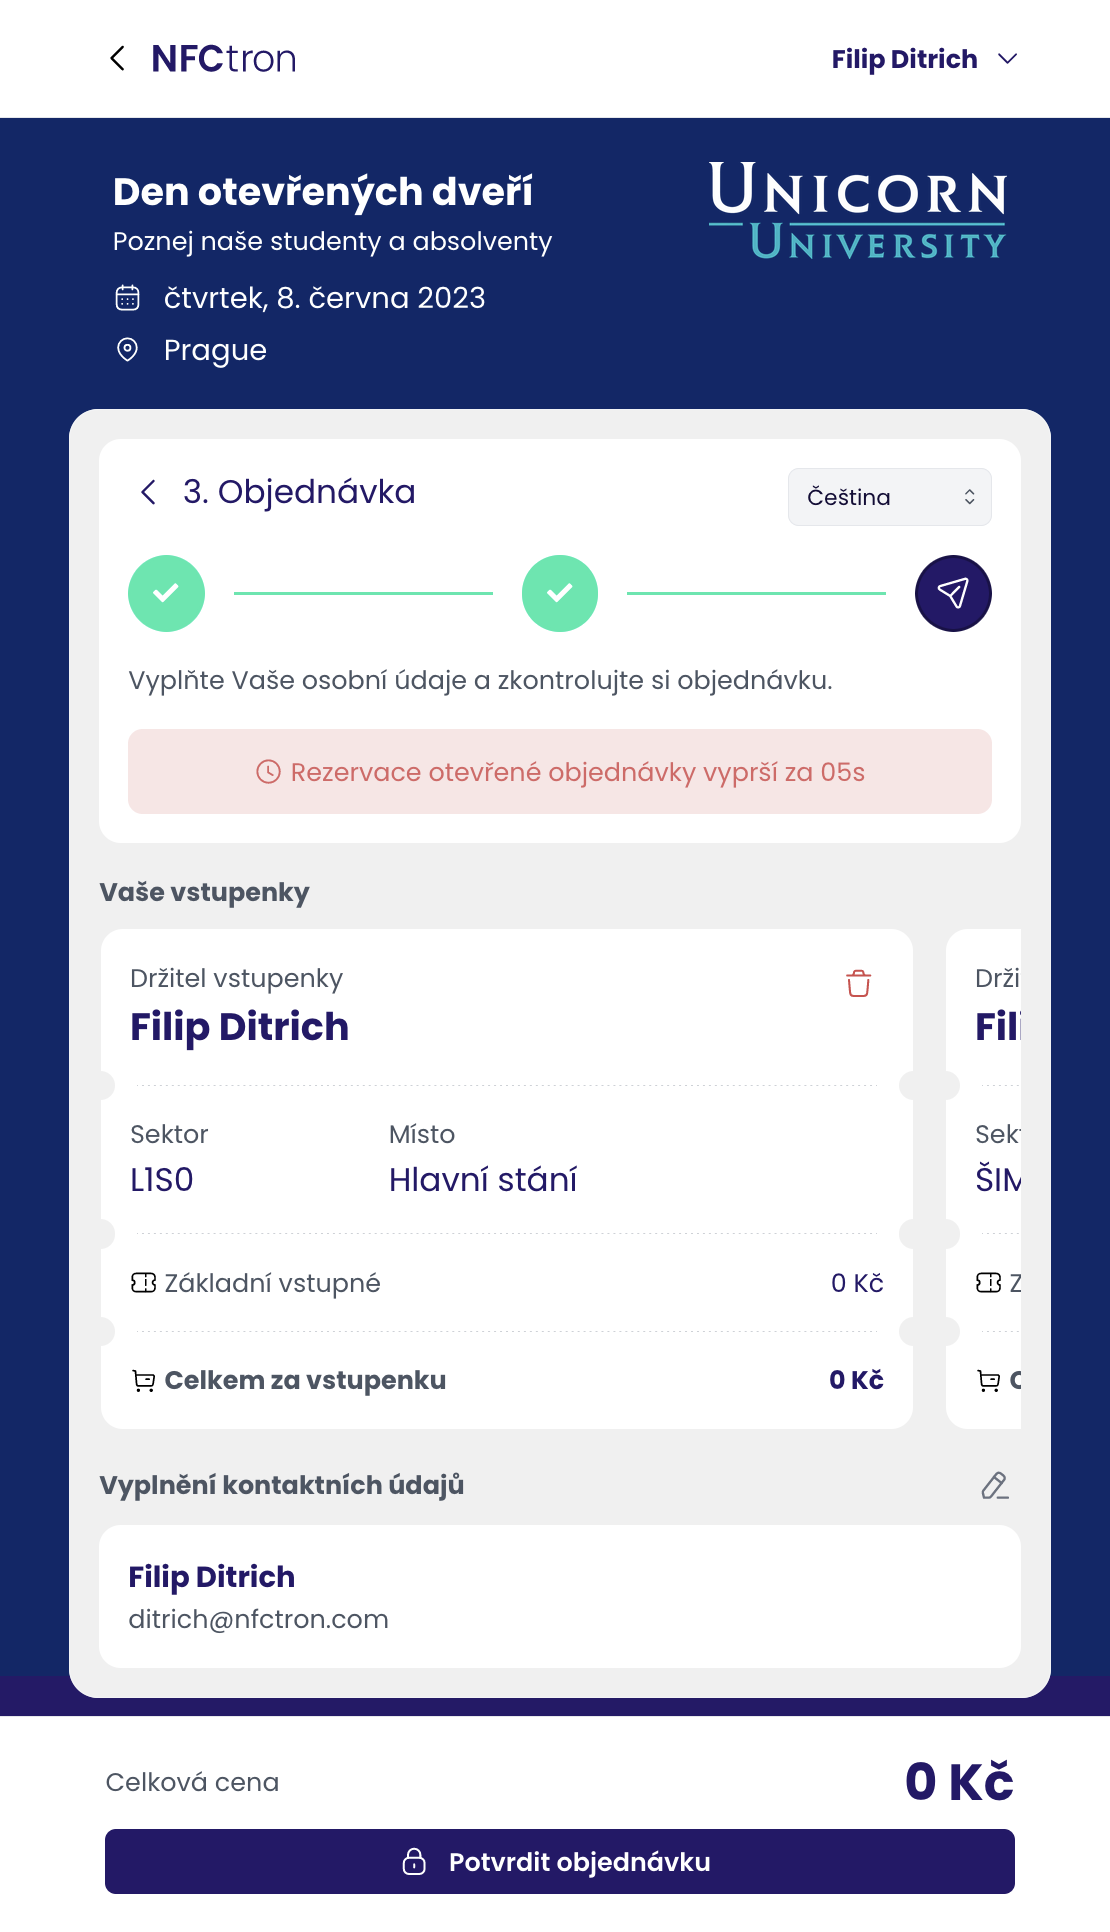
\includegraphics[width=\textwidth]{\FIGDIR/nfctron-tickets-reservation-expiring}
        \caption{Blížící se expirace}
        \label{fig:nfctron-tickets-reservation-expiring}
    \end{subfigure}
    \hfill
    \begin{subfigure}{0.3\textwidth}
        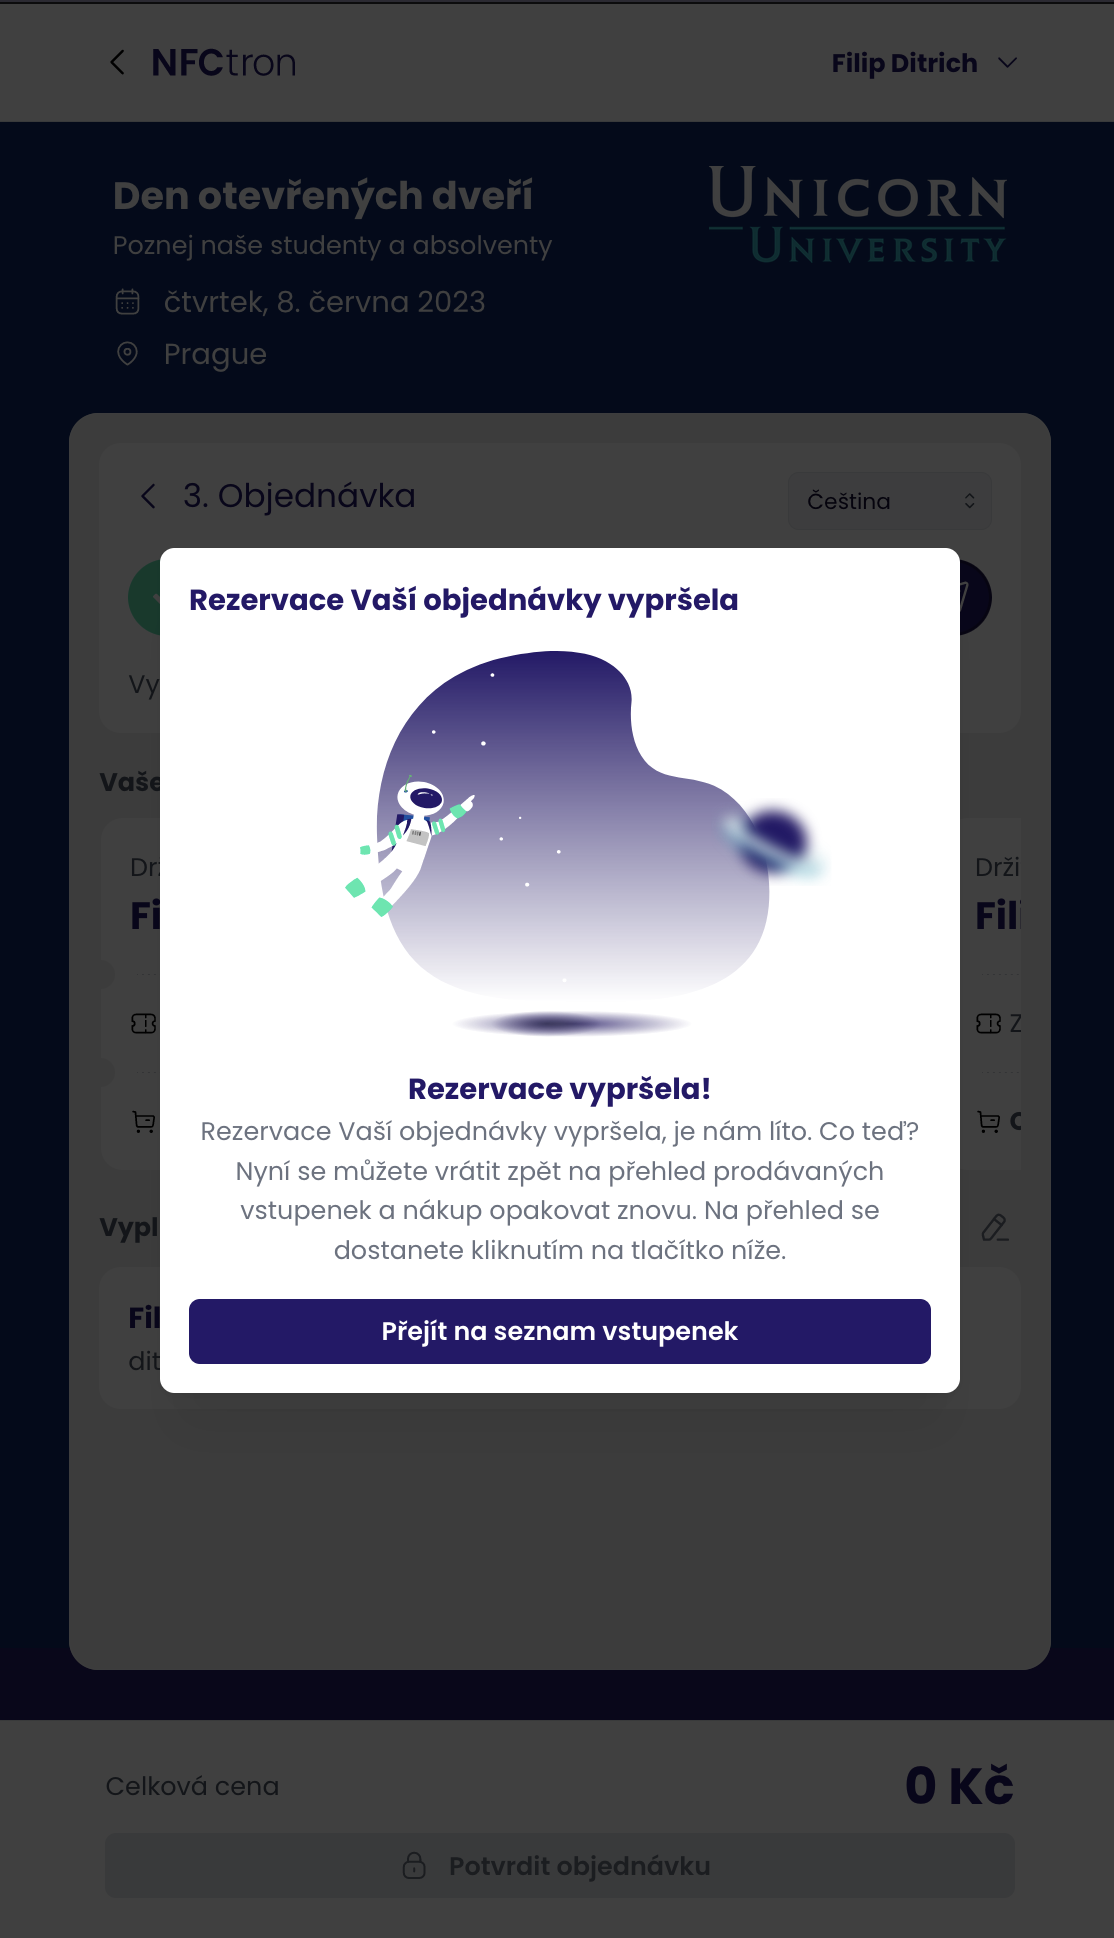
\includegraphics[width=\textwidth]{\FIGDIR/nfctron-tickets-reservation-expired}
        \caption{Expirovaná rezervace}
        \label{fig:nfctron-tickets-reservation-expired}
    \end{subfigure}

    \caption{Rezervační mechanismus služby NFCtron Tickets na zkušební akci}
    \label{fig:nfctron-tickets-reservation}
\end{figure}

%%% TODO: Sekce - Dokončení objednávky
%%% --------------------------------------------------------------
\section{Dokončení objednávky}
\label{sec:specifikace-dokonceni-objednavky}
Jakmile si zákazník vybere požadované vstupenky a rezervovaná místa, je jeho posledním úkolem dokončit a tím tak vytvořit objednávku, kteoru následně zaplatí.
Tento proces je většinou rozdělen do několika kroků, které zákazníka postupně provedou celým procesem dokončení objednávky.

Tato podkapitola se bude těmito kroky zabývat a bude se snažit popsat jejich jednotlivé části a funkčnosti, které by měly být v takovémto systému implementovány.

Avšak je nutné nejprve uvést, že následující funkčnosti jsou v práci uvedené pouze z důvodu kompletnosti představení celého procesu nákupu vstupenek s rezervací míst a záměrně nebudou v rámci praktické části plně implementovány nýbrž pouze orientačně využity – a to z důvodu toho, že se jedná již převážně o funkčnosti a procesy na straně backednového systému a ne frontendového, který je předmětem této práce.

%%% TODO: Podsekce - Osobní informace
%%% --------------------------------------------------------------
\subsection{Osobní informace}
\label{sec:specifikace-dokonceni-objednavky-osobni-informace}
Pro účely dokončení objednávky je nutné, aby si zákazník vyplnil své osobní informace, které jsou potřebné pro vytvoření objednávky a následné doručení vstupenek. Tyto informace by měly obsahovat minimálně následující údaje:

\begin{itemize}
    \item Jméno a příjmení
    \item Emailová adresa
    \item Telefonní číslo
\end{itemize}

Tyto informace jsou nezbytné například pro odeslání potvrzení objednávky, doručení vstupenek či poskytování případné podpory zákazníkům.

Někteří poskytovatelé stále nabízí doručení fyzických vstupenek na adresu zákazníka, nicméně tento způsob je spíše přežitek. V dnešní moderní době je výhodnější i ekologičtější využít možnost digitálních vstupenek, které zákazník obdrží v elektronické podobě například prostřednictvím emailu či SMS zprávy.

V rámci dokončení objednávky je také časté vybídnutí zákazníka k dokončení registrace na dané platformě či službě, přes kterou vstupenky nakupuje. Tato registrace je většinou dobrovolná, ale může být i povinná, pokud chce zákazník využít některé z výhod, které jsou s touto registrací spojeny.

%%% TODO: Podsekce - Výběr platební metody
%%% --------------------------------------------------------------
\subsection{Výběr platební metody}
\label{sec:specifikace-dokonceni-objednavky-vyber-platebni-metody}
Proces dokončení objednávky by v posledním kroku měl zákazníkovi nabídnout několik možností platby. Nejčastěji se jedná o platební metody jako:

\begin{itemize}
    \item platba kartou
    \item platba přes PayPal
    \item platba přes Apple Pay
    \item platba přes Google Pay
    \item platba přes bankovní převod
\end{itemize}

\begin{figure}[H]
    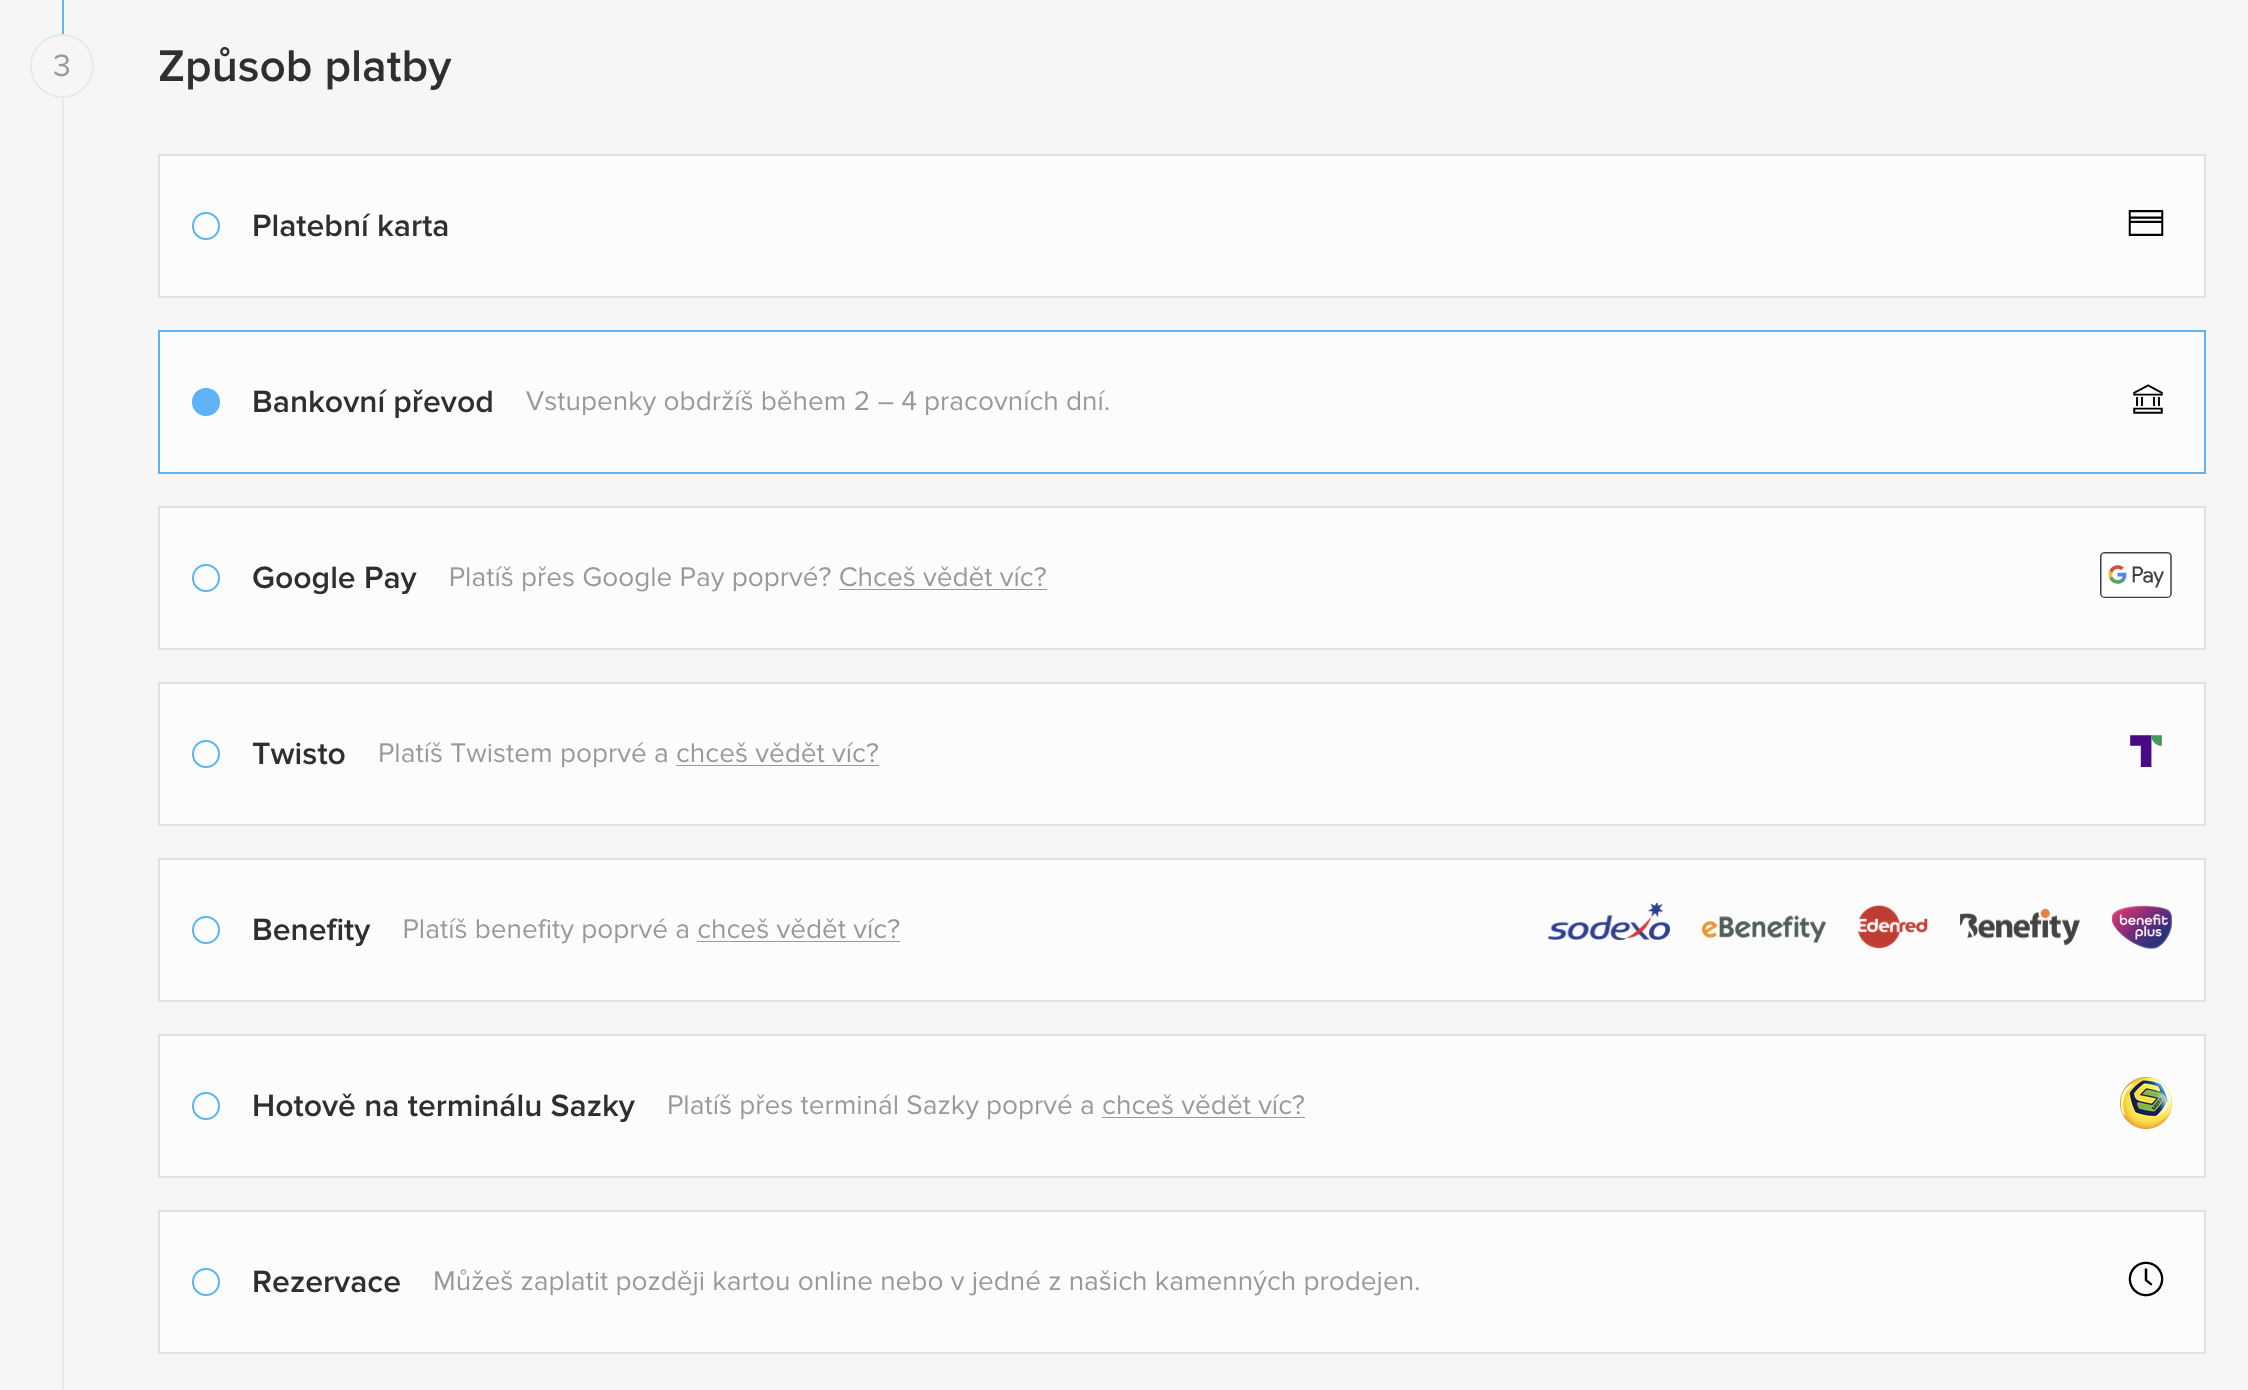
\includegraphics[width=\linewidth]{\FIGDIR/goout-payment-methods}
    \centering
    \caption{Vyběr platební metody na GoOut.net}
    \label{fig:goout-payment-methods}
\end{figure}

Na obrázku \ref{fig:goout-payment-methods} je vidět výběr platební metody ve službě GoOut.net, která nabízí výše zmíněné platební metody\footnote{platební metoda Apple Pay zde není uvedena, jelikož je dostupná pouze v rámci prohlížečů Safari: \url{https://support.apple.com/guide/iphone/use-apple-pay-in-apps-app-clips-and-safari-iph67e89f7c8/ios}} spolu i dalšími jako například platba přes službu Twisto či Sodexo a další jiné benefitní programy.

Pro účely platby kartou je nutné, aby byl zákazník přesměrován na platební bránu, která je schopna tuto platbu zpracovat.
Většinou se jedná o platební brány třetích stran, které jsou schopny zpracovat platby z různých platebních karet a poskytovatelů.
Mezi nejznámější poskytovatele platebních brán na českém trhu patří například:

\begin{itemize}
    \item \emph{Comgate} (\url{https://www.comgate.cz/platebni-brana})
    \item \emph{GoPay} (\url{https://www.gopay.com/cs/})
    \item \emph{PayU} (\url{https://czech.payu.com/payu-moderni-platebni-reseni/})
    \item \emph{GP webpay} (\url{https://www.gpwebpay.cz/})
    \item \emph{Stripe} (\url{https://stripe.com/en-cz})
\end{itemize}

Na obrázcích~\ref{fig:comgate-fees-table} a~\ref{fig:comgate-payment-methods} je vidět, že každý poskytovatel platební brány nabízí jiné výhody a poplatkové modely, nicméně všechny mají společné to, že zpracovávají platby z různých platebních karet a poskytovatelů a přímo podporují i mobilní platby přes Apple Pay a Google Pay.

\begin{figure}[H]
    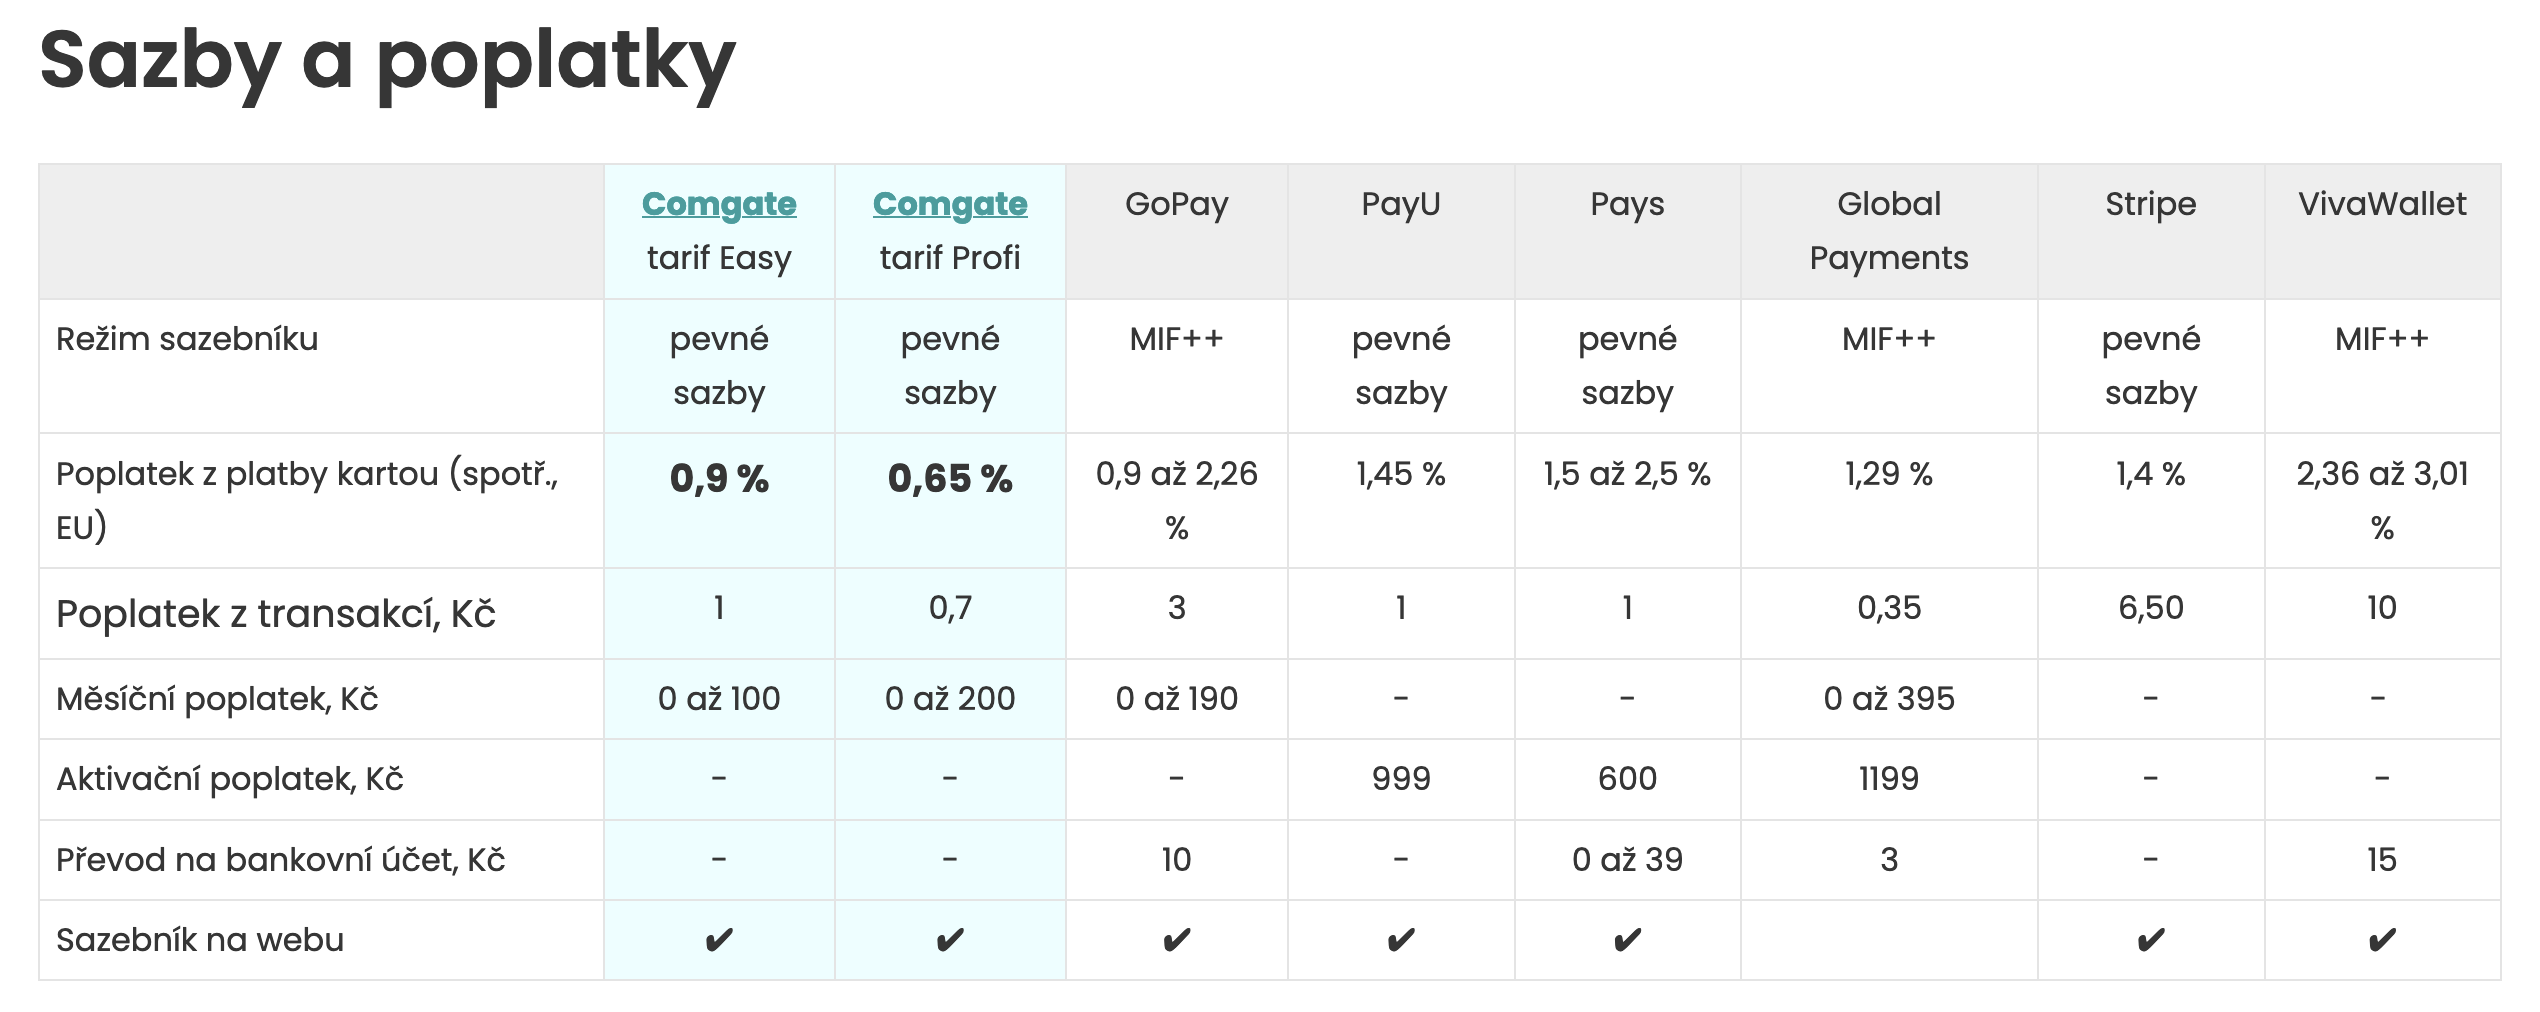
\includegraphics[width=\linewidth]{\FIGDIR/comgate-fees-table}
    \centering
    \caption{Srovnání platebních bran dle Comgate.cz~\cite{comgate_srovnani_platebnich_bran}}
    \label{fig:comgate-fees-table}
\end{figure}

\begin{figure}[H]
    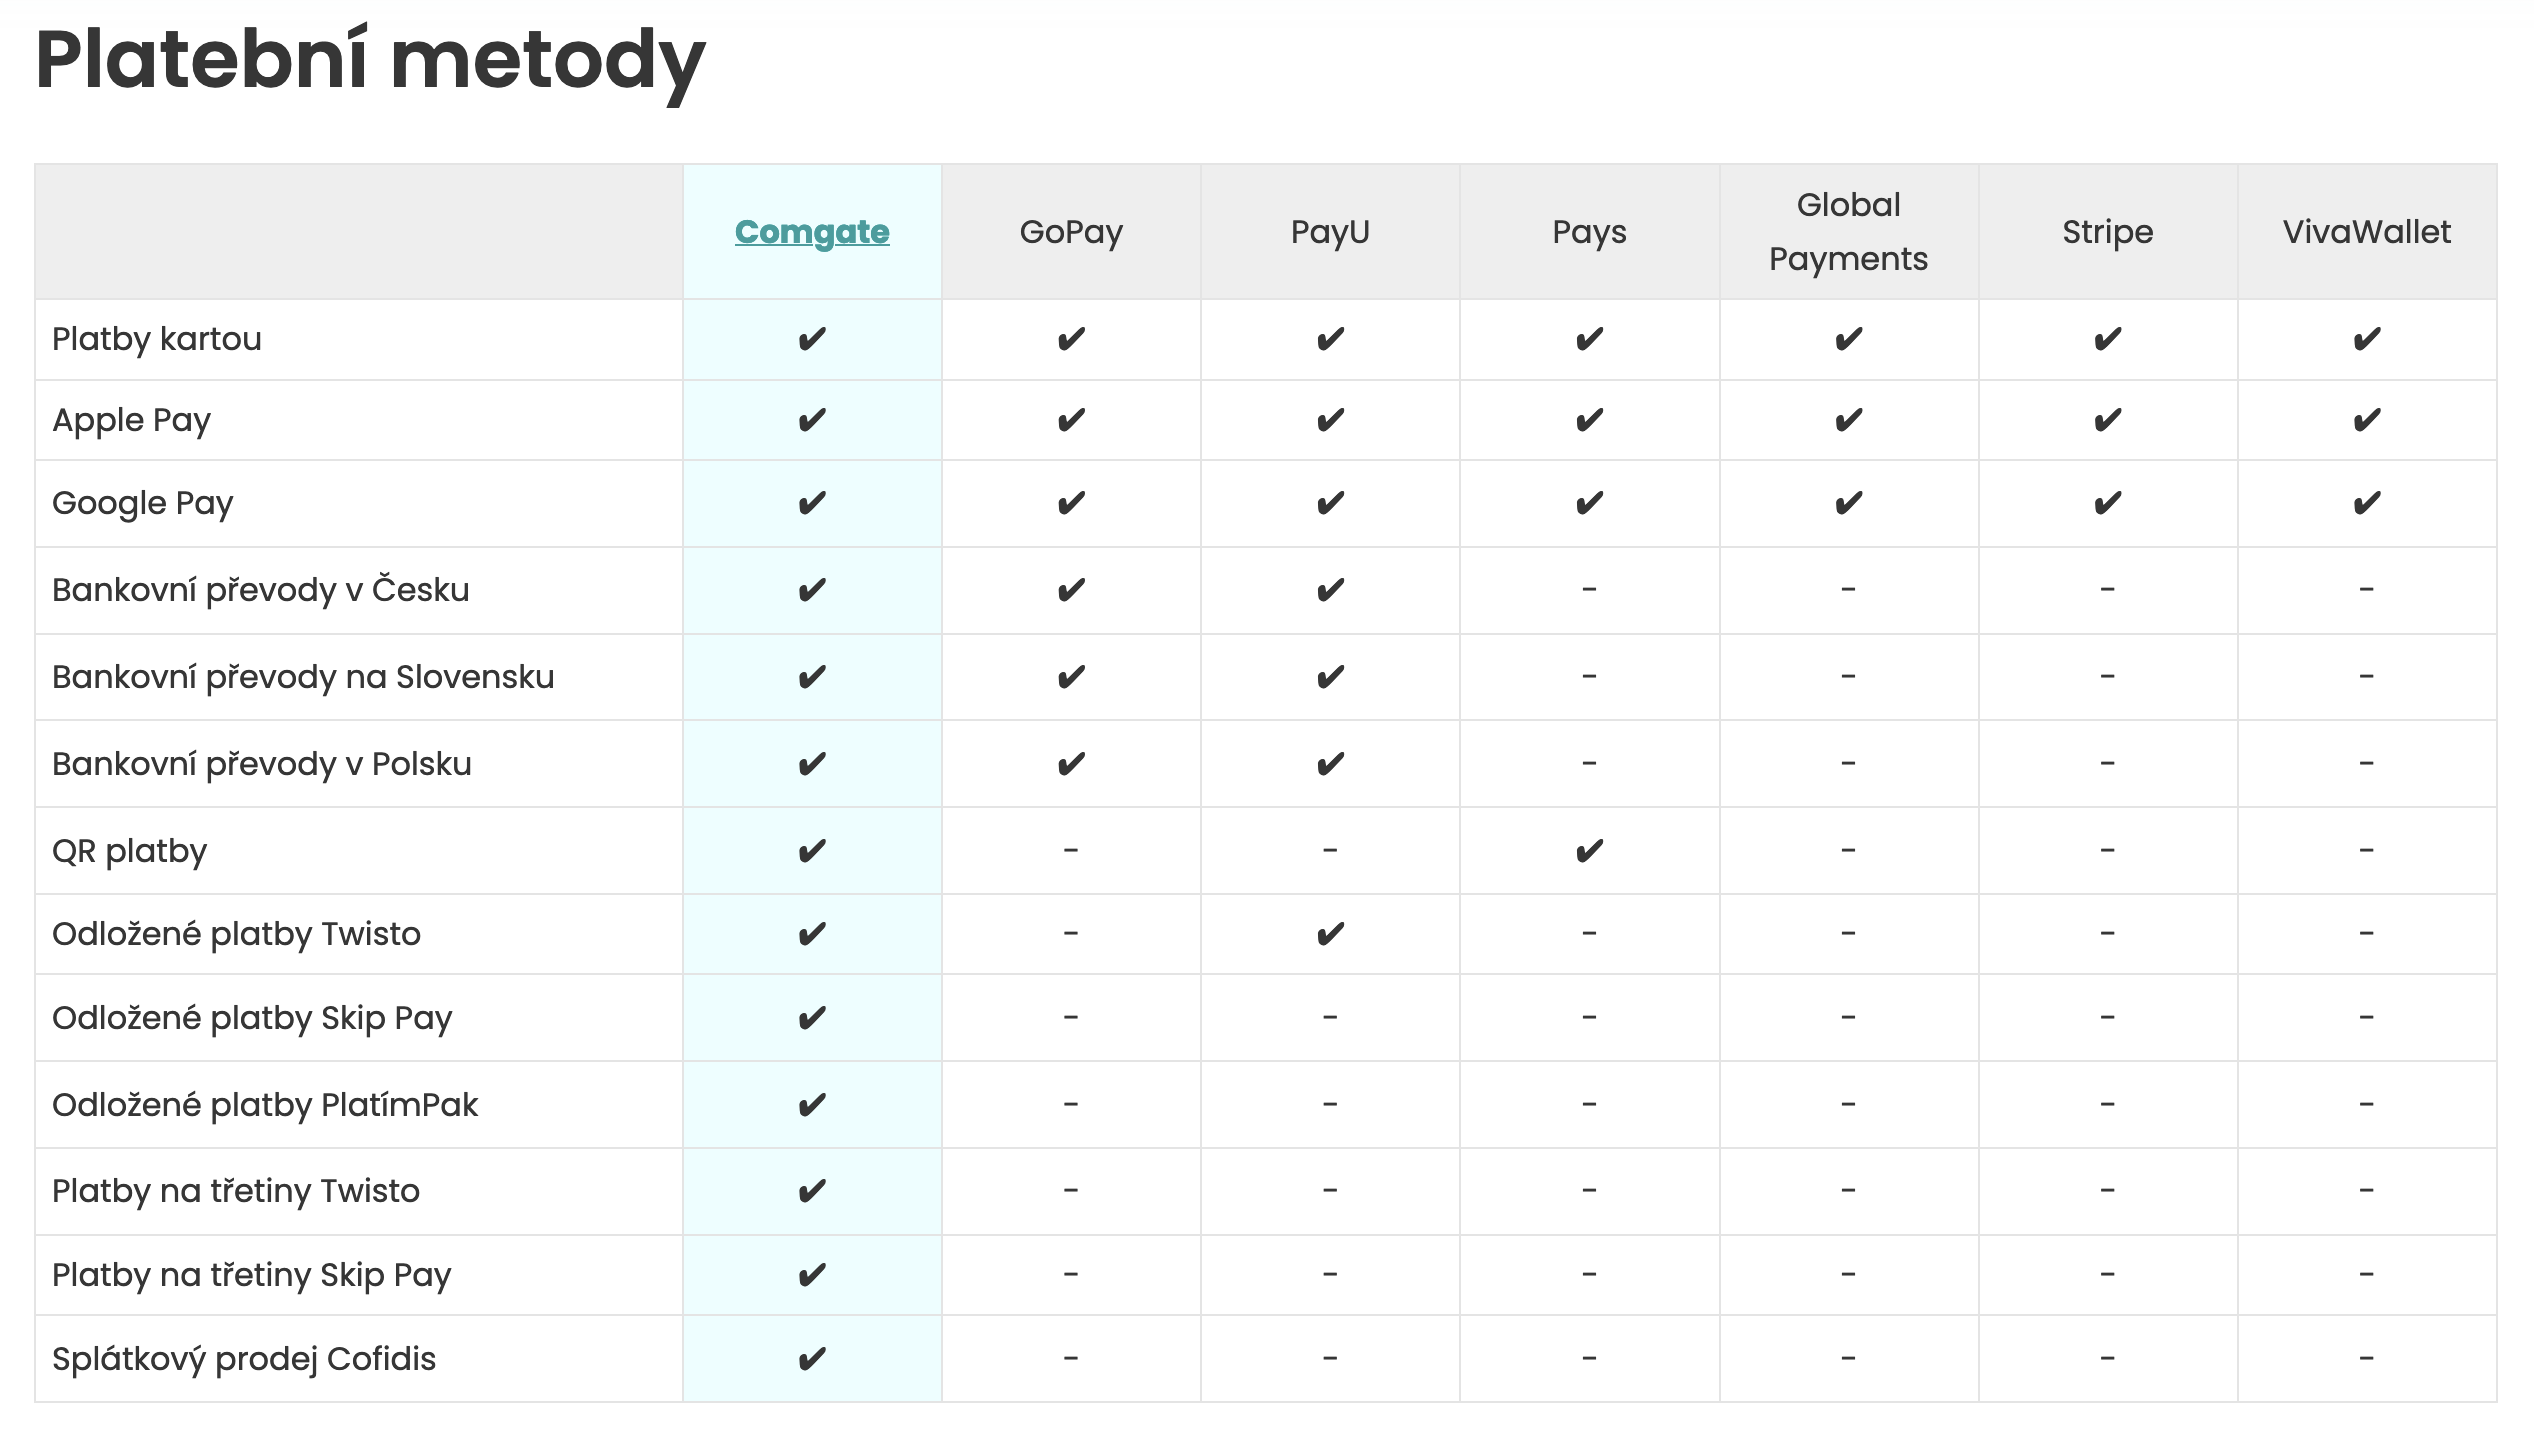
\includegraphics[width=\linewidth]{\FIGDIR/comgate-payment-methods}
    \centering
    \caption{Platební metody poskytované platebními poskytovateli dle Comgate.cz~\cite{comgate_srovnani_platebnich_bran}}
    \label{fig:comgate-payment-methods}
\end{figure}

Některé e-shopy však nabízí i vlastní platební bránu, nicméně tato možnost je spíše výjimkou.
Stát se provozovatelem vlastní platební brány je totiž velmi náročné na vývoj, udržbu a provoz a je k němu nutné mít i licenci platební instituce (PI)~\cite{schejbal_platebni_instituce}, kterou vydává Česká národní banka (ČNB)~\cite{cnb_dohled_platebni_instituce}.

Platby přes bankovní převod mohou být pro poskytovatele řešení prodeje vstupenek velmi výhodné, jelikož se jedná o levnější způsob převodu peněz, než je tomu u plateb kartou.
Platební brány si totiž účtují poplatky za zpracování každé z plateb a to nejčastěji v režimu pevného sazebníku či MIF++ modelu\footnote{někdy také označován jako Interchange++}, který rozděluje poplatky mezi vydavatelskou bankou, karetním schématem (např.\ Visa, MasterCard) a platební bránou.

Do nedávna byla platba bankovním převodem pro zákazníky stále méně oblíbená, jelikož bylo nutné počkat na připsání peněz na účet poskytovatele, což mohlu trvat i několik dní.
V dnešní době je však možné využít tzv. instantní platby, které jsou schopny převést peníze mezi účty různých bank během několika sekund.
V České republice aktuálně podporuje instantní platby již několik bank, jako například Komerční banka, a.s., MONETA Money Bank, a.s.\ či Fio banka, a.s.\ a další\footnote{kompletní seznam účastníků okamžitých plateb dle ČNB dostupný z: \url{https://www.cnb.cz/export/sites/cnb/cs/platebni-styk/.galleries/certis/download/seznam_okamzite_platby.pdf}}.

Pro účely této práce, jak bylo již zmíněno na začátku podsekce \ref{sec:specifikace-dokonceni-objednavky}, bude backendový systém celou funkčnost plateb pouze simulovat a nebude se snažit o integraci s žádnou platební bránou.


%%% TODO: Podsekce - Souhrn objednávky
%%% --------------------------------------------------------------
\subsection{Souhrn objednávky}
\label{sec:specifikace-dokonceni-objednavky-souhrn-objednavky}
Po vyplnění všech potřebných informací a výběru platební metody by zákazníkovi měl být před finálním potvrzením objednávky zobrazen její souhrn.
Tento souhrn zákazníkovi umožní zkontrolovat, zda jsou všechny údaje správně vyplněné a zda je vše v pořádku.
Pokud zákazník zjistí, že je něco špatně, měl by mít možnost vrátit se zpět a údaje opravit.
Pokud je vše v pořádku, měl by mít možnost objednávku potvrdit a přejít k platebnímu procesu.

Součástí potrvzení objednávky také často bývá zaškrtnutí souhlasu se zpracováním osobních údajů a obchodních podmínek či i případně dalších informací, jako například zasílání novinek a reklamních nabídek na e-mailovou adresu zákazníka.

%%% TODO: Podsekce - Vytvoření objednávky a potvrzení
%%% --------------------------------------------------------------
\subsection{Vytvoření objednávky a potvrzení}
\label{sec:specifikace-dokonceni-objednavky-vytvoreni-objednavky-a-potvrzeni}
Po potvrzení objednávky by měla být vytvořena objednávka v databázi a zákazníkovi by mělo být zobrazeno potvrzení o jejím vytvoření.
Na základě vybrané platbní metody by měl být dále přesměrován k jejímu zaplacení a posléze zpět na detail objednávky s potrvzením o zaplacení.
Při úspěšné platbě by zákazníkovi měl systém doručit zakoupené vstupenky v elektronické podobě, například v podobě PDF souboru, který bude obsahovat vstupenky ve formátu QR kódu.

    %%%%% Kapitola 4 - Návrh uživatelského rozhraní
%%%%% ------------------------------------------------------------
\chapter{Návrh uživatelského rozhraní}
\label{ch:navrh-uzivatelskeho-rozhrani}
Ve světě digitálních produktů a jejich designu jsou uživatelské rozhraní, z anglického \foreign{\acf{ui}}, a uživatelský zážitek, z anglického \foreign{\acf{ux}}, dva pojmy, které se často zaměňují, ačkoli se jedná o velmi odlišné aspekty procesu vývoje produktu.
Tato kapitola si klade za cíl představit koncepty \ac{ui} a \ac{ux}, prozkoumat jejich vzájemný vztah a zabývat se specifiky návrhu \ac{ui} pro aplikaci pro prodej vstupenek s rezervací míst.

\textbf{\ac{ui}} se vztahuje k vizuálním prvkům produktu, se kterými uživatel interaguje – tedy tlačítkům, textu, ikonografii, formulářům a všem vizuálním prvkům, které umožňují uživateli interagovat s produktem.
V kontextu aplikace pro prodej vstupenek s rezervací míst se \ac{ui} vztahuje například k interaktivnímu plánu sedaček, výběru vstupenek, tlačítku pro přechod k dokončení objednávky nebo nákupnímu košíku.

\textbf{\ac{ux}} je na druhou stranu celkový zážitek uživatele při interakci s produktem.
Je ovlivněn snadností použití, hodnotou, kterou uživatel z produktu získává, a emocemi, které jsou při interakci vyvolány.
\ac{ux} bere v potaz celou cestu uživatele, od okamžiku, kdy uživatel do aplikace vstoupí, až po okamžik, kdy dokončí nákup.

Významným aspektem \ac{ux} je uživatelská cesta, z anglického \foreign{User Journey}, která popisuje cestu uživatele při interakci s produktem.
Uživatelská cesta se skládá z jednotlivých kroků, které uživatel musí absolvovat, aby dosáhl svého cíle.

Souhra \ac{ui} a \ac{ux} je v procesu návrhu produktu klíčová.
Dobře navržené \ac{ui} usnadňuje \ac{ux}.
Například intuitivně navržený plán sedadel (\ac{ui}) může proces výběru sedadla zpříjemnit a zjednodušit (\ac{ux}).

Následující sekce této kapitoly prozkoumají základní principy návrhu \ac{ui} a možná použití Maslowovy hierarchie, za účelem návrhu rozhraní více zaměřeného na uživatele.
Dále budou uvedeny a porovnány různé nástroje, které jsou k dispozici pro návrh \ac{ui} a důvody rozhodnutí pro konkrétní nástroj.
Následně budou analyzovány specifikace prototypu z kapitoly~\ref{ch:specifikace} z hlediska \ac{ui}/\ac{ux} se zaměřením na tzv.\ uživatelské příběhy, které tvoří základ \ac{ux} designu.

Závěr této kapitoly bude věnován návrhu interaktivního plánu sedaček, který je klíčovým \ac{ui} prvkem vyvýjeného prototypu aplikace.

%%% Sekce - Principy návrhu uživatelského rozhraní
%%% --------------------------------------------------------------
\section{Principy návrhu uživatelkého rozhraní}
\label{sec:navrh-principy}
Návrh uživatelského rozhraní je poměrně rozsáhlá disciplína, která se zaměřuje na vizuální a interaktivní aspekty produktu.
Při návrhu \ac{ui} je důležité dodržovat určité principy, které zajišťují optimální uživatelskou zkušenost.
Tato sekce shrnuje některé základní principy návrhu \ac{ui} a posuzuje jejich implikace v kontextu aplikace pro prodej vstupenek s rezervací míst.

\textbf{Konzistence}: Tento princip prosazuje zachování jednotnosti napříč všemi prvky \ac{ui}.
Konzistence se projevuje v použití podobných prvků, akcí a designu napříč celým rozhraním.
Například pokud určitá barva značí interaktivní prvek na plánu sedadel, stejná barva by měla být použita i pro značení interaktivních prvků jinde v rámci aplikace.
Tímto se zvyšuje předvídatelnost, což uživatelům usnadňuje orientaci a navigaci v rozhraní.

\textbf{Uživatel v kontrole}: Základním principem návrhu \ac{ui} je umožnit uživateli cítit se vždy v kontrole nad produktem.
Toho lze dosáhnout návrhem transparentního a intuitivního systému, ve kterém uživatel vždy ví, kde se nachází a jak postupovat.
V kontextu aplikace pro prodej vstupenek to může znamenat poskytnutí jasného a zřejmého způsobu, jak uživatelé mohou přejít k výběru sedadla, přidání do košíku a dokončení objednávky.

\textbf{Zpětná vazba}: Zpětná vazba je klíčovým aspektem každé interakce, protože potvrzuje nebo informuje  uživatele o vykonaných akcích.
Vizuální indikátory, jako je zvýraznění vybraného sedadla nebo potvrzovací zpráva při přidání vstupenky do košíku, poskytují uživateli okamžitou zpětnou vazbu.
Tím se snižuje nejistota a zvyšuje se důvěra uživatele v rozhraní.

\textbf{Jednoduchost}: Návrh \ac{ui} by měl směřovat k jednoduchosti.
Čím méně úsilí musí uživatel vynaložit na pochopení rozhraní, tím lepší bude celková uživatelská zkušenost.
Čisté, jednoduché rozhraní s jasným zaměřením na funkčnost snižuje kognitivní zátěž a zvyšuje použitelnost.

\textbf{Prevence a řešení chyb}: Chyby jsou nevyhnutelné v jakékoli interakci, ale dobře navržené \ac{ui} může zabránit většině uživatelských chyb nebo zjednodušit jejich řešení.
To může znamenat například zakázání tlačítka \textit{Pokračovat} dokud není vybráno sedadlo nebo zobrazení jasných a užitečných chybových zpráv, když něco selže.

\textbf{Afordance a signifikance}: \foreign{Afordance} se vztahuje k vlastnosti objektu, která naznačuje, jak se má používat.
\foreign{Signifikance} jsou vizuálními nápovědami k témto \foreign{afordancím}.
Například sedadlo na plánu sedadel může být navrženo tak, aby naznačovalo, že na něj lze kliknout (\foreign{afordance}), a změna kurzoru při najetí na sedadlo (\foreign{signifikance}) může tuto zprávu posílit.

Pochopení a aplikace těchto základních principů návrhu \ac{ui} je klíčové pro vytvoření intuitivního a uživatelsky přívětivého rozhraní.
Tyto principy řídí rozhodnutí v rámci návrhu a pomáhají návrhu \ac{ui} s celkovým cílem poskytnout uživatelům bezproblémový zážitek z rezervace vstupenek.
Další sekce se zabývá tím, jak lze hierarchii Maslowa aplikovat pro další zlepšení uživatelsky orientovaného návrhu.

%%% Sekce - Aplikovaná psychologie na návrh uživatelských rozhraní
%%% --------------------------------------------------------------
\section{Aplikovaná psychologie na UI/UX}
\label{sec:navrh-psychologie}

\epigraph{\textit{``Some people say, "Give the customers what they want." But that's not my approach. Our job is to figure out what they're going to want before they do.''}}{-- Steve Jobs}

Proces návrhu uživatelského rozhraní se netýká pouze estetiky nebo funkcionality v izolaci.
Ve skutečnosti, k vytvoření rozhraní, které skutečně rezonuje s uživateli, si lze vypůjčit koncept z psychologie - Maslowovu hierarchii potřeb.
Tato hierarchie, obvykle vizualizovaná jako pyramidová struktura, ilustruje cestu jednotlivce k seberealizaci a naplnění, začínající od základních fyziologických potřeb až po složitější emoční a psychologické potřeby.

\textit{Maslowova hierarchie potřeb} je teorie psychologa Abrahama Maslowa, která se snaží vysvětlit, co motivuje lidi.
Maslow tvrdil, že lidé mají potřeby, které se snaží uspokojit, ale některé z nich jsou naléhavější než jiné.
Když jsou tyto potřeby uspokojeny, lidé se mohou cítit šťastnější, ale když nejsou, lidé mohou být frustrovaní a nespokojení.\cite{maslow}
Maslow rozdělil lidské potřeby do pěti základních úrovní, které jsou znázorněny na obrázku~\ref{fig:maslow} níže.

\begin{figure}[H]
    \centering
    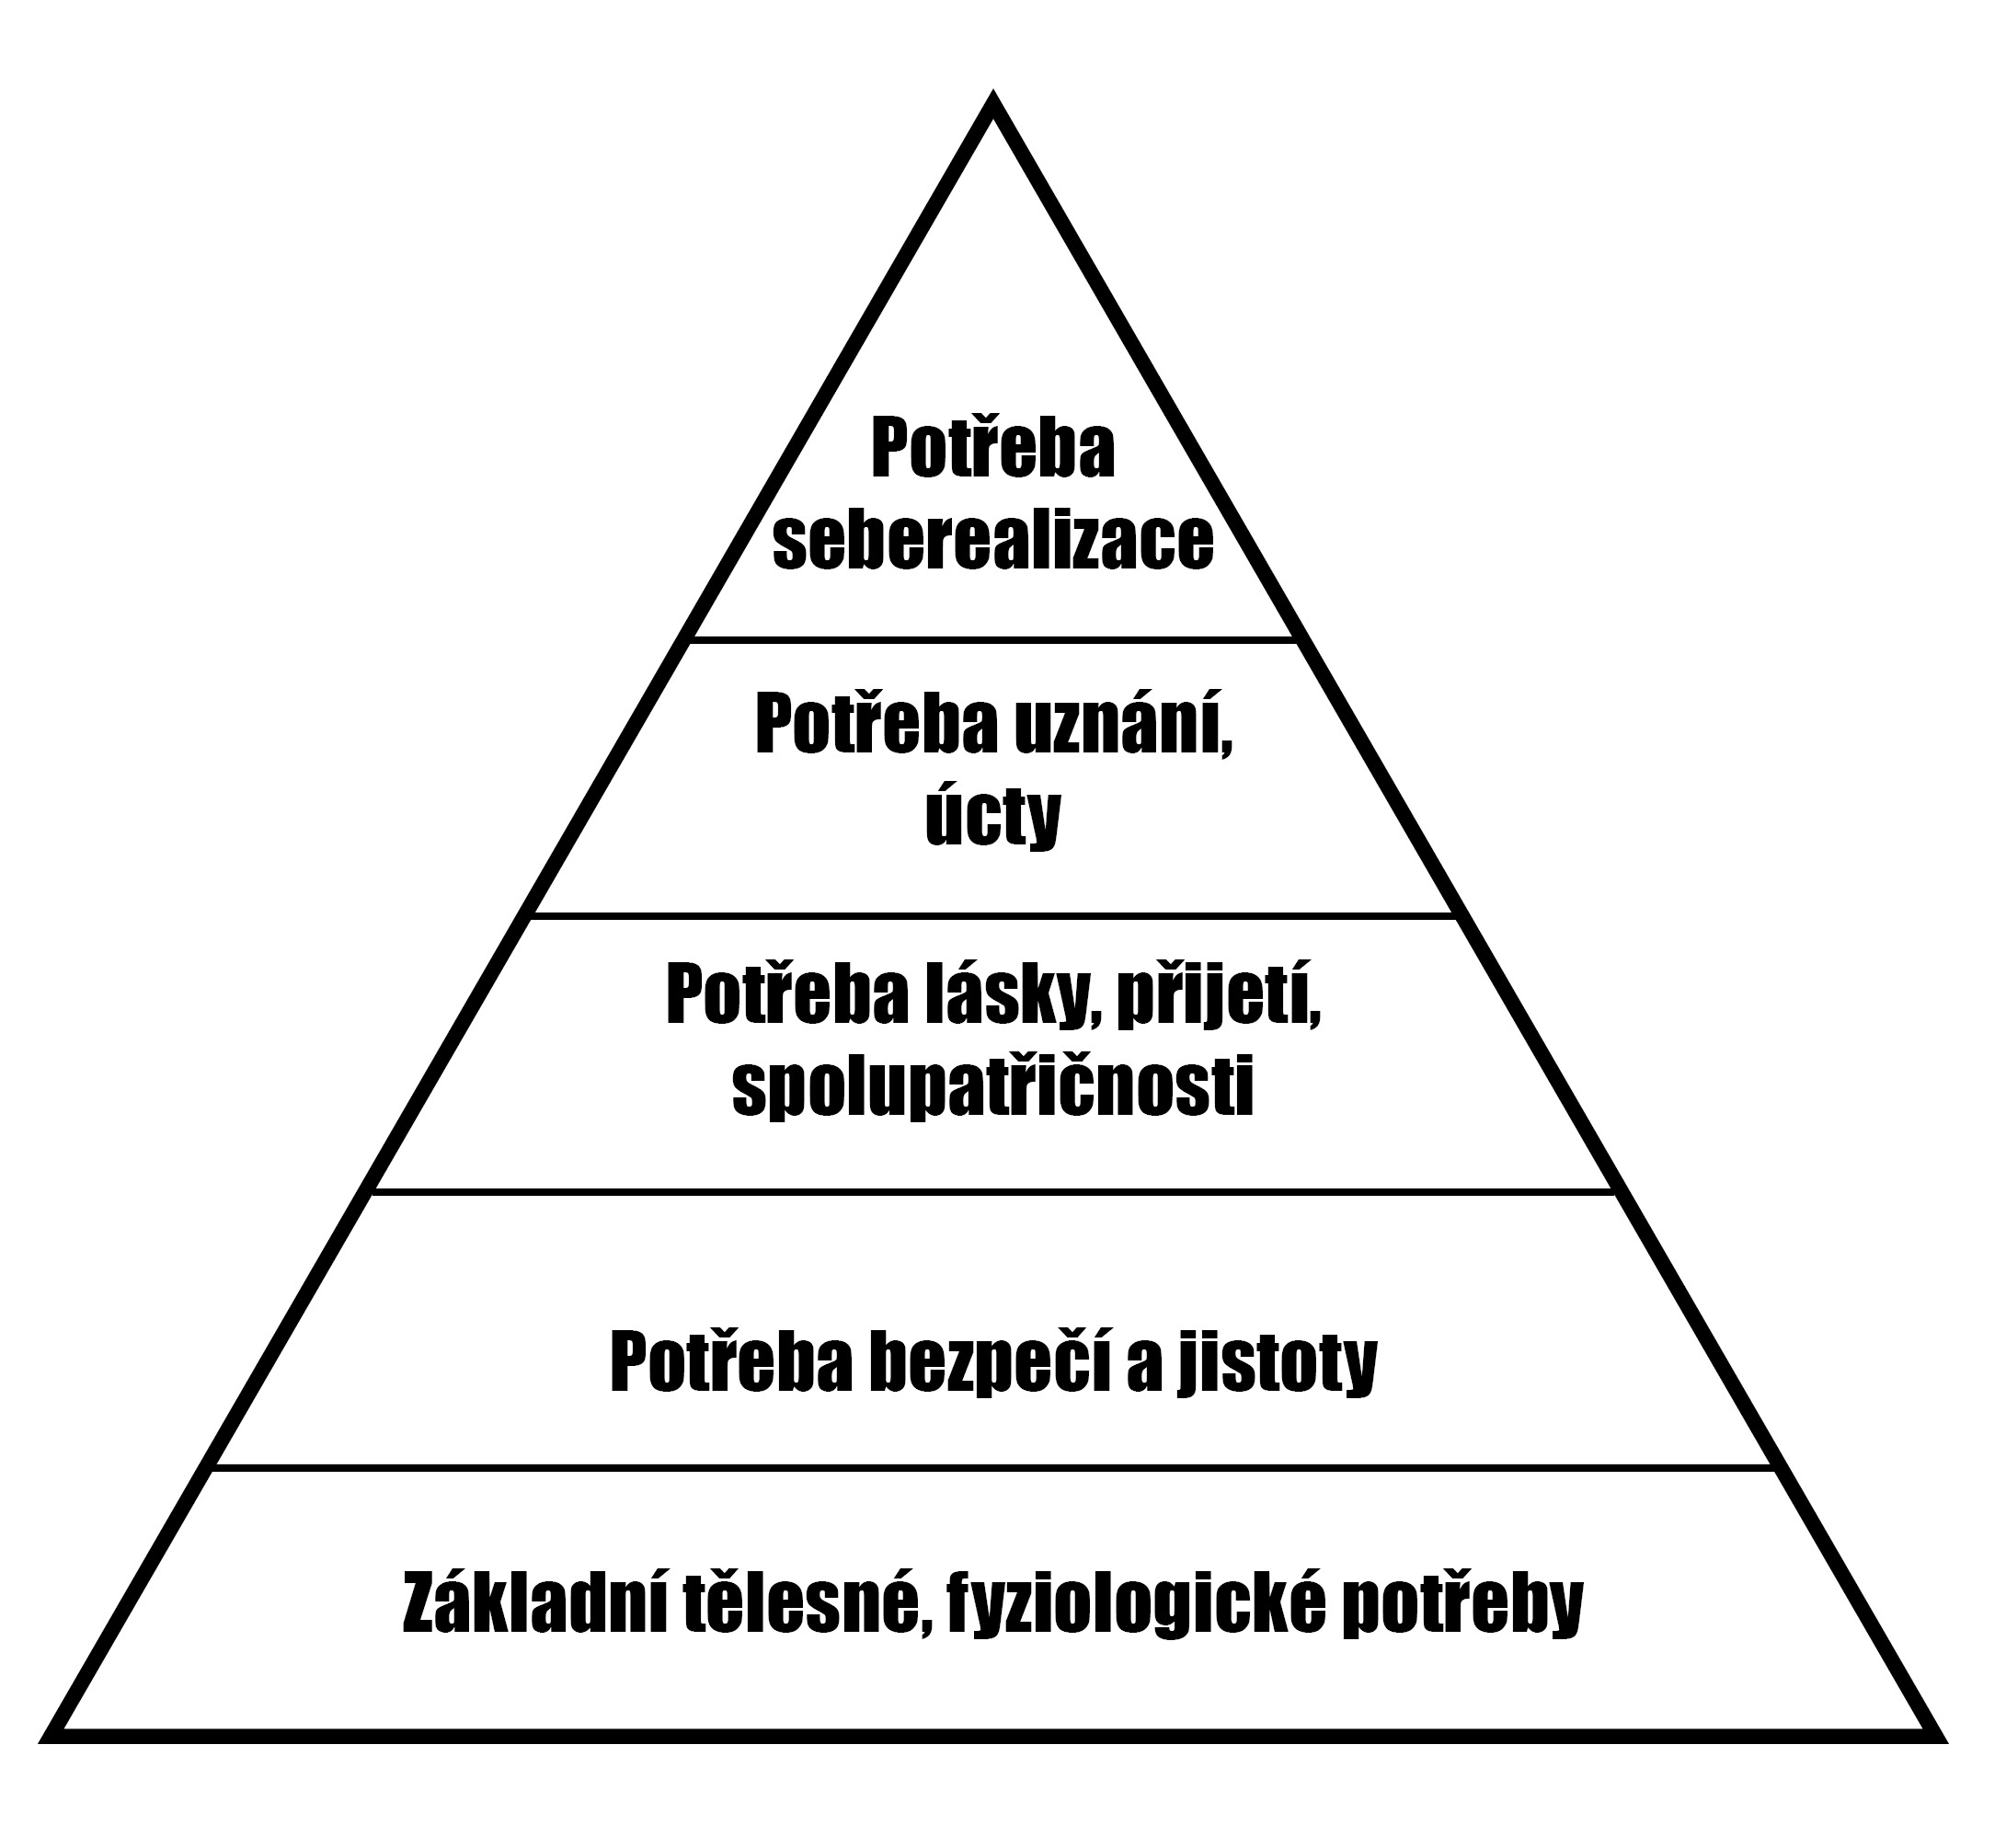
\includegraphics[width=0.8\textwidth]{\FIGDIR/maslow}
    \caption{Maslowova hierarchie potřeb\cite{wiki_potreby}}
    \label{fig:maslow}
\end{figure}

\begin{enumerate}
    \item \textbf{Fyziologické potřeby}: základní potřeby pro přežití, jako je potrava, voda, teplo a spánek
    \item \textbf{Potřeby bezpečí}: potřeby, které se týkají bezpečnosti a zabezpečení
    \item \textbf{Sociální potřeby}: potřeby, které se týkají příslušnosti, lásky a přátelství
    \item \textbf{Potřeby uznání}: potřeby, které se týkají úcty a sebeúcty
    \item \textbf{Potřeby seberealizace}: potřeby, které se týkají osobního růstu a rozvoje
\end{enumerate}

Jak to tedy ale souvisí s návrhem \ac{ui} a zejména s návrhem aplikace pro prodej vstupenek?

\textbf{Maslowova hierarchie potřeb} může být aplikována na návrh \ac{ui} tak, že každá úroveň hierarchie představuje jeden základní aspekt návrhu \ac{ui}.

V roce 2010 navrhl Steven Bradley v článku \textit{Designing For A Hierarchy Of Needs} podobnou hierarchii specificky pro design, se pěti odpovídajícími úrovněmi znázorněnými na obrázku~\ref{fig:design-hierarchy-of-needs}.\cite{bradley_hierarchy_of_needs}

\begin{figure}[H]
    \centering
    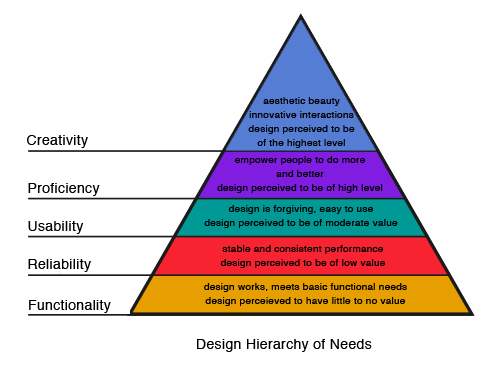
\includegraphics[width=0.8\textwidth]{\FIGDIR/design-hierarchy-of-needs}
    \caption{Hierarchie potřeb v návrhu \ac{ui} dle Stevena Bradleyho\cite{bradley_hierarchy_of_needs}}
    \label{fig:design-hierarchy-of-needs}
\end{figure}

\textbf{Funkčnost}: Na základě pyramidy jsou základní fyziologické potřeby.
V kontextu návrhu \ac{ui} to znamená základní funkčnost.
Aplikace musí fungovat tak, jak se očekává, aby si uživatelé mohli vybrat sedadlo, přidat vstupenku do košíku a dokončit proces objednávky bez jakýchkoli problémů.
Základní funkčnost musí být spolehlivá a robustní.

\textbf{Spolehlivost}: Další úroveň pyramidy je bezpečnost, která se v návrhu \ac{ui} týká spolehlivosti.
Rozhraní by mělo být navrženo tak, aby se uživatelé cítili bezpečně a sebevědomě při interakci s ním.
Poskytování jasných pokynů, okamžité zpětné vazby a potvrzení o úspěšných akcích (například přidání vstupenky do košíku) přispívá k pocitu bezpečí a použitelnosti.

\textbf{Použitelnost}: Střední část pyramidy pokrývá sociální potřeby, které se v \ac{ui} termínech rovnají uživatelské spokojenosti.
Esteticky příjemné rozhraní, personalizovaný uživatelský zážitek a interaktivní prvky (jako interaktivní plán sedadel) mohou významně zvýšit uživatelskou spokojenost.

\textbf{Odbornost}: Potřeby sebeúcty zahrnují touhu po uznání a respektu.
V kontextu aplikace pro prodej vstupenek by to mohlo znamenat přidání funkcí, které překračují očekávání uživatelů a zpříjemňují jim zážitek.
Může se jednat o něco tak jednoduchého, jako je blahopřání po úspěšném nákupu, nebo vizuální animace při výběru sedadla.

\textbf{Kreativita}: Na vrcholu pyramidy se nachází seberealizace, která se týká realizace osobního potenciálu a hledání osobního růstu a vrcholných zážitků.
Uživatelské rozhraní by mohlo přispět k této potřebě tím, že uživatelům umožní kreativně řešit problémy a dosáhnout svých cílů.
Například nabízení návrhů na nejlepší dostupná sedadla nebo podobných akcí může uživatele posílit a zlepšit jejich zážitek.

Použití Maslowovy hierarchie pro návrh \ac{ui} aplikace pro prodej vstupenek může pomoci zajistit, aby návrh splňoval potřeby uživatelů na různých úrovních.
Z počátku je nutné zajistit základní funkčnosti a spolehlivost, aby uživatelé mohli využívat aplikaci bez jakýchkoli problémů.
Dále je nutné zaměřit se na použitelnost, aby byl proces výběru sedadla a nákupu vstupenky co nejvíce zjednodušen.
Při postupu v hierarchii se budou zkoumat různé metody, jak zvýšit uživatelskou spokojenost a zlepšit jejich zážitek.
Cílem na vrcholu tohoto procesu je navrhnout rozhraní, které vyvažuje praktičnost a uživatelskou přívětivost, zatímco zároveň zajišťuje vizuální přitažlivost a emoční zapojení.
To povede k přínosnějšímu, uspokojivějšímu a úspěšnějšímu uživatelskému zážitku.

Další sekce se bude zabývat nástroji dostupnými pro návrh \ac{ui} a o důvodech pro výběr konkrétního nástroje pro tento projekt.

%%% TODO: Sekce - Nástroje pro návrh
%%% --------------------------------------------------------------
\section{Nástroje pro návrh}
\label{sec:navrh-ui-nastroje}
V oblasti návrhu uživatelského rozhraní má návrhář k dispozici širokou škálu nástrojů.
Tyto nástroje usnadňují nízkoúrovňové i vysokoúrovňové prototypování, přičemž každý z nich představuje jedinečnou sadu vlastností přispívajících k tvorbě, spolupráci a testování návrhů.
Tato sekce stručně popisuje tři nejčastěji používané nástroje pro návrh uživatelského rozhraní, a to Figma, Adobe XD a Sketch.

%%% TODO: Podsekce - Figma
%%% --------------------------------------------------------------
\subsection{Figma}
\label{subsec:navrh-ui-nastroje-figma}
Figma je nástroj pro návrh uživatelského rozhraní, který funguje v prohlížeči a je založen na cloudových technologiích.
Jeho hlavními výhodami jsou platformní nezávislost a snadná spolupráce.
Figma je také vybavena sadou funkcí, které usnadňují návrh uživatelského rozhraní, jako je vektorové kreslení, prototypování a předávání vývojářům.
\cite{figma}

\begin{figure}[H]
    \centering
    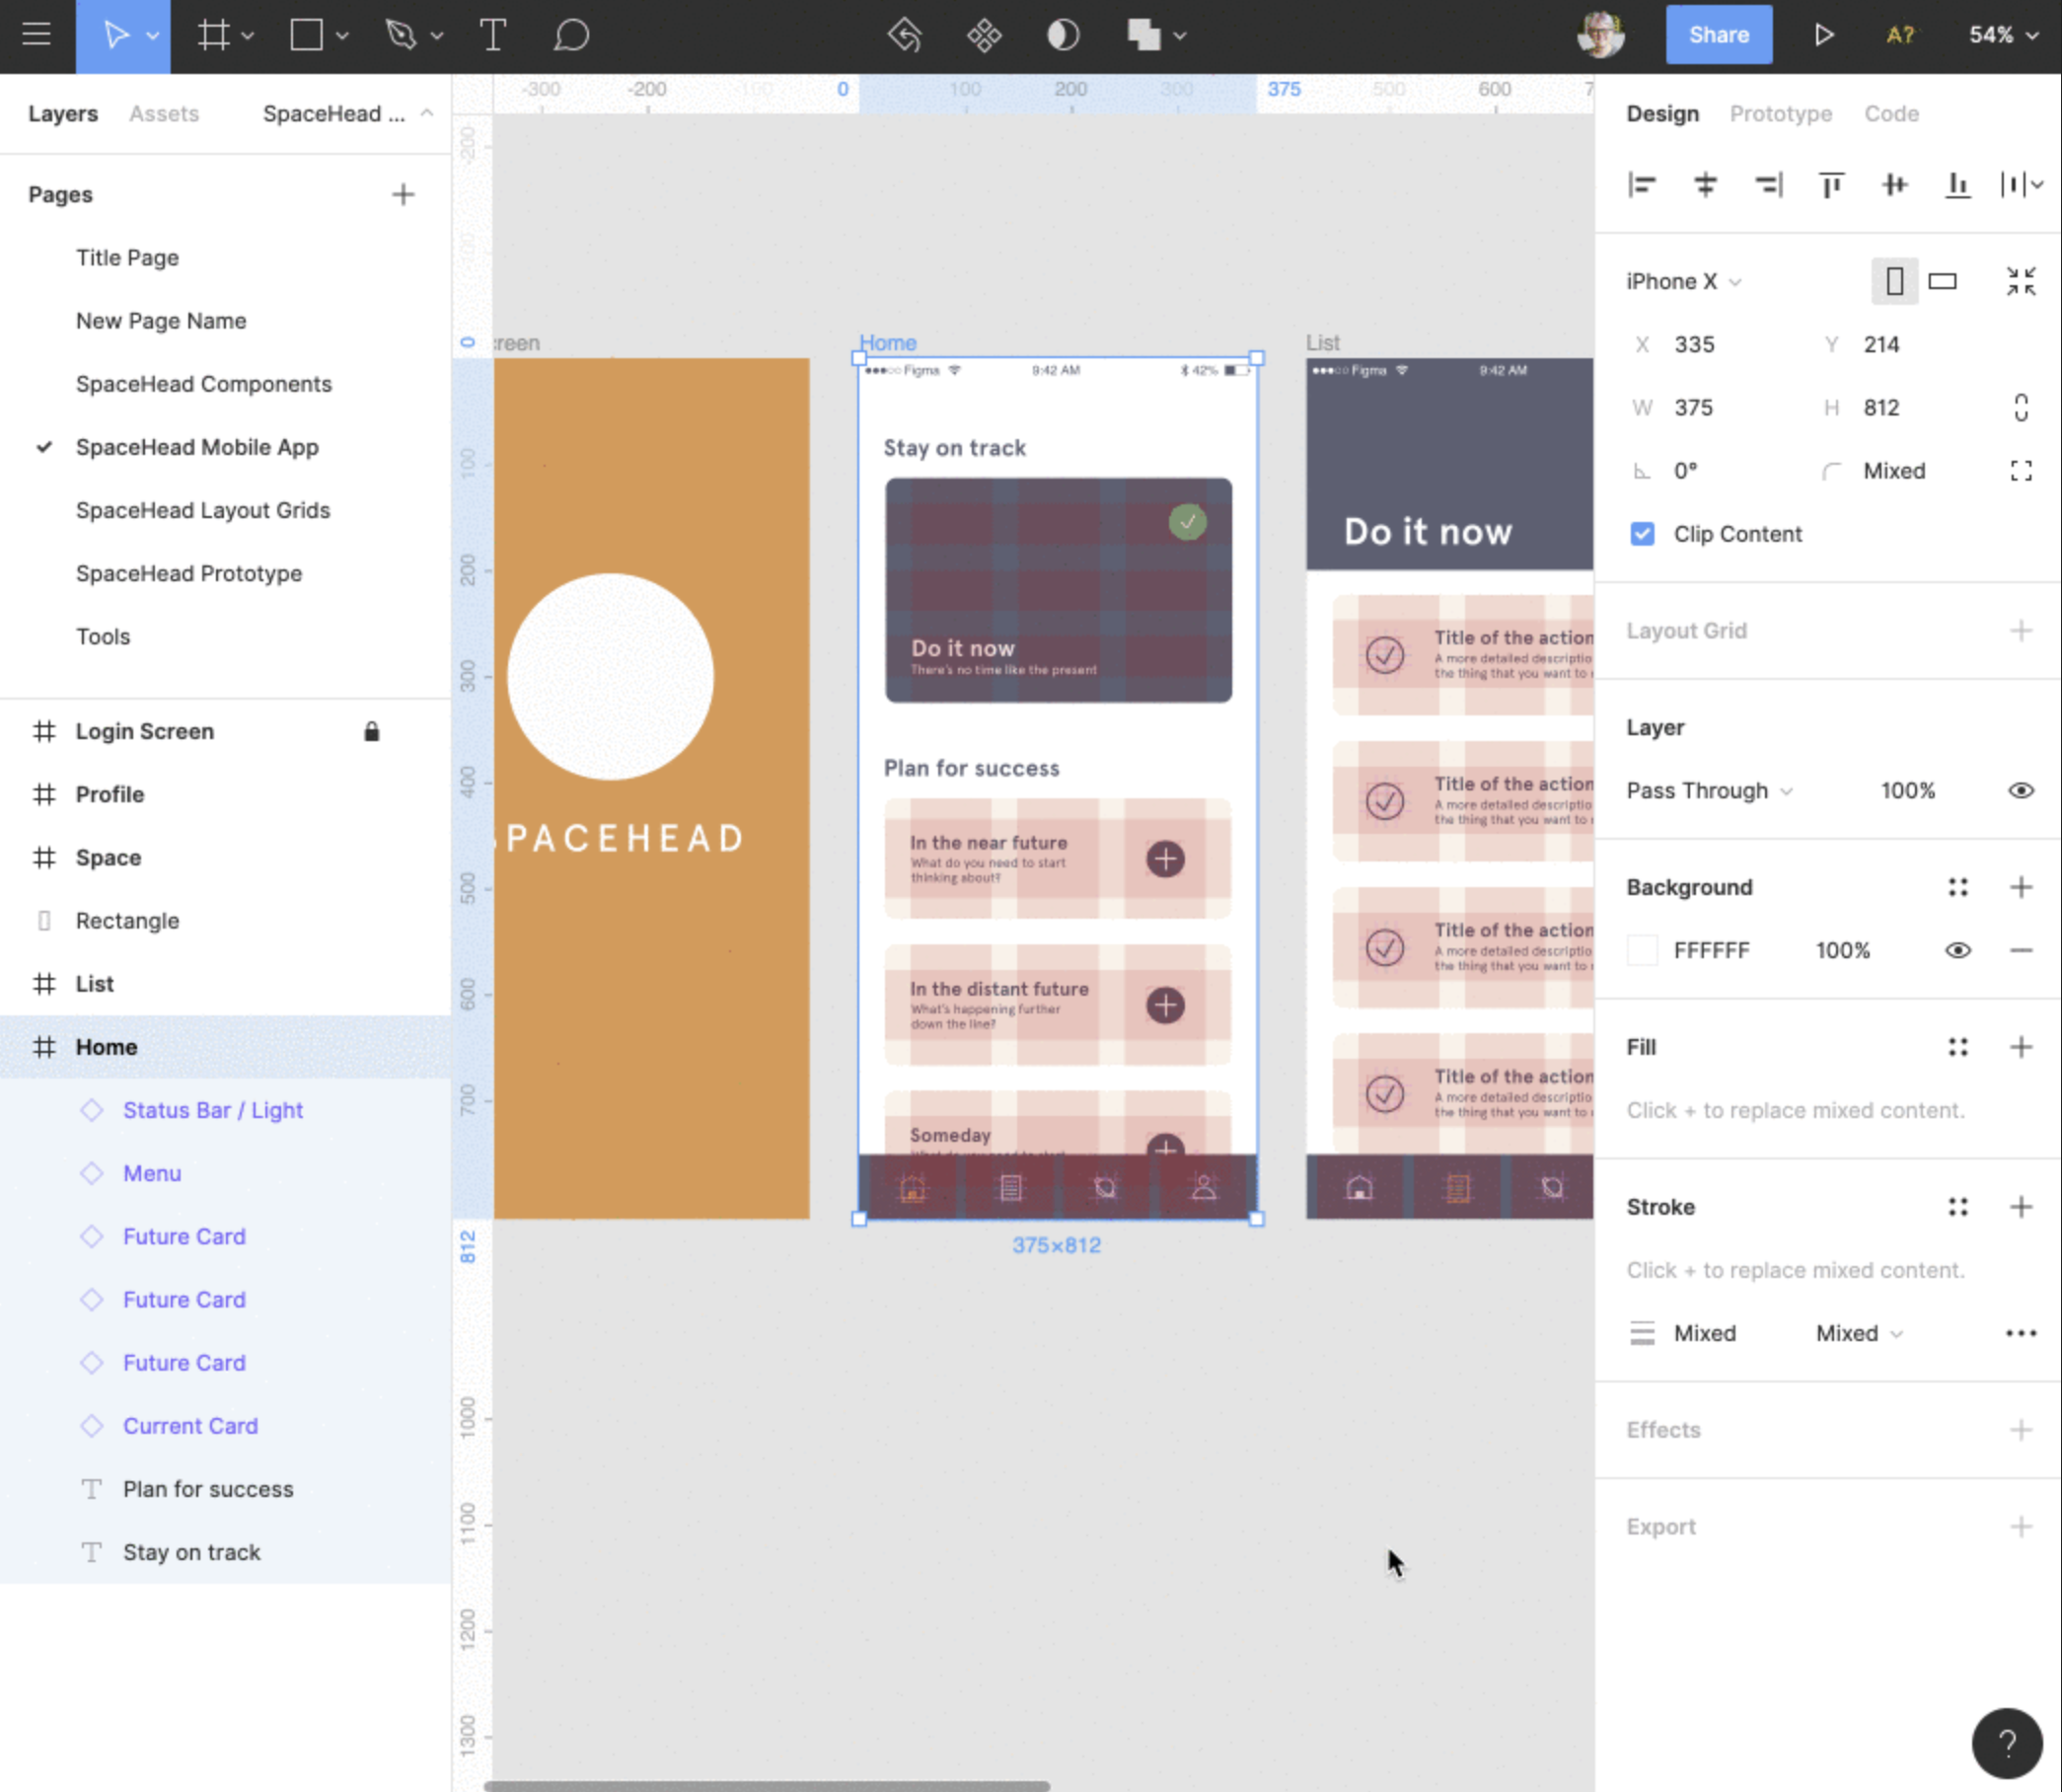
\includegraphics[width=0.8\textwidth]{\FIGDIR/figma}
    \caption{Ukázka nástroje Figma\cite{figma}}
    \label{fig:figma}
\end{figure}

%%% TODO: Podsekce - Adobe XD
%%% --------------------------------------------------------------
\subsection{Adobe XD}
\label{subsec:navrh-ui-nastroje-adobe-xd}
Adobe XD je nástroj od společnosti Adobe pro návrh uživatelského rozhraní, který funguje na platformách Windows i MacOS.
Jeho hlavními výhodami jsou jednoduché uživatelské rozhraní, prototypování a snadná integrace s ostatními produkty Adobe Suite.
\cite{adobe-xd}

\begin{figure}[H]
    \centering
    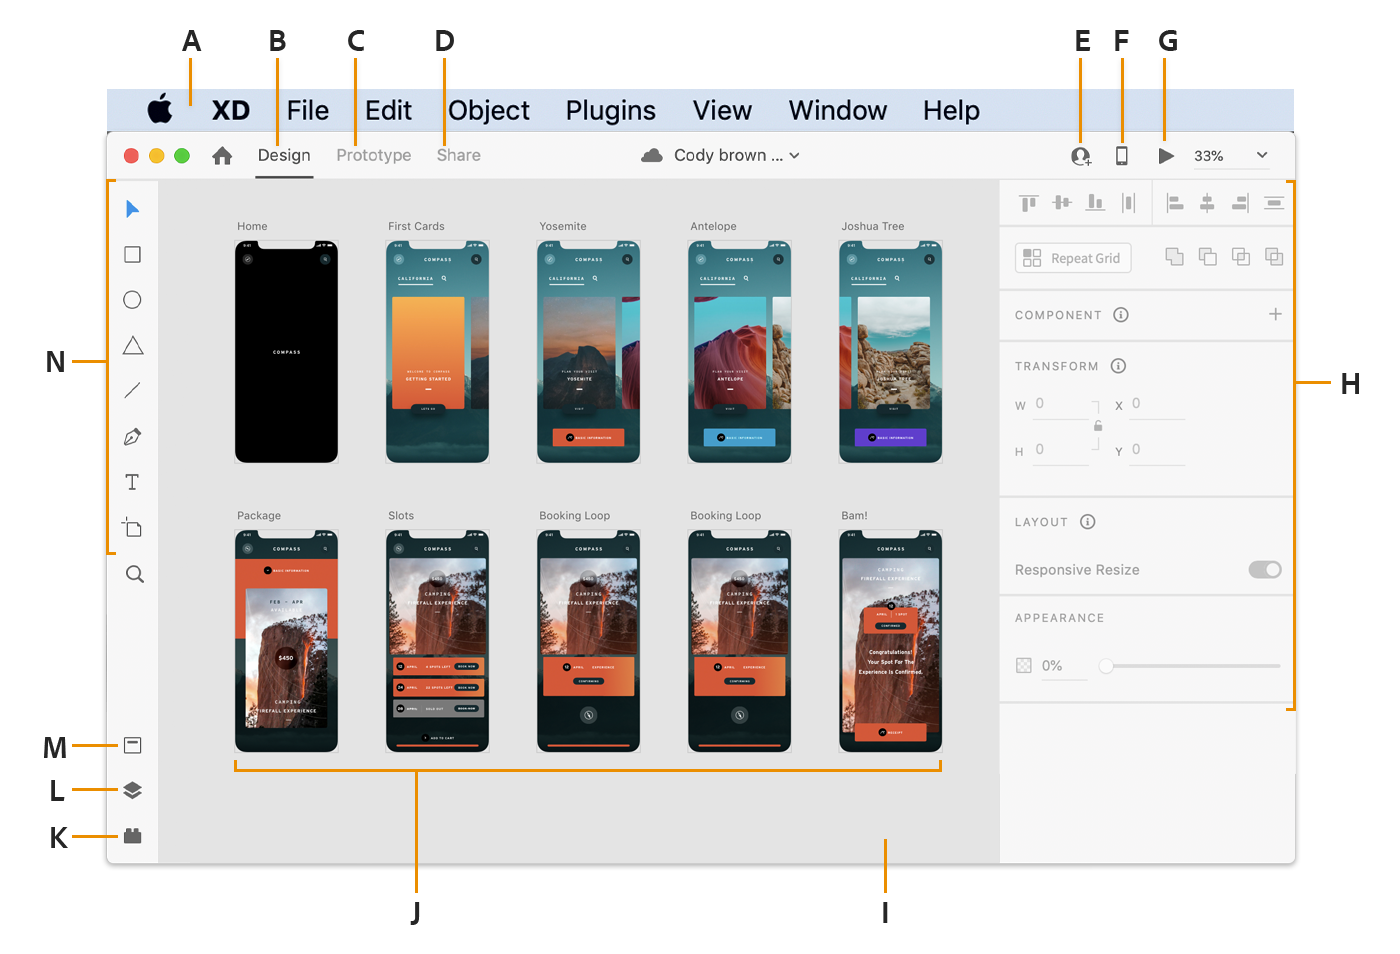
\includegraphics[width=0.8\textwidth]{\FIGDIR/adobe-xd}
    \caption{Ukázka nástroje Adobe XD\cite{adobe-xd}}
    \label{fig:adobe-xd}
\end{figure}

%%% TODO: Podsekce - Sketch
%%% --------------------------------------------------------------
\subsection{Sketch}
\label{subsec:navrh-ui-nastroje-sketch}
Sketch je nástroj pro návrh uživatelského rozhraní, který funguje výhradně na platformě MacOS.
Je to vektorový nástroj, který je chválen pro svou jednoduchost a rychlost.
Je užitečný při tvorbě rozhraní, webových stránek a ikon, i když absence vestavěných prototypovacích schopností může být pro některé návrháře omezujícím faktorem.
\cite{sketch}

\begin{figure}[H]
    \centering
    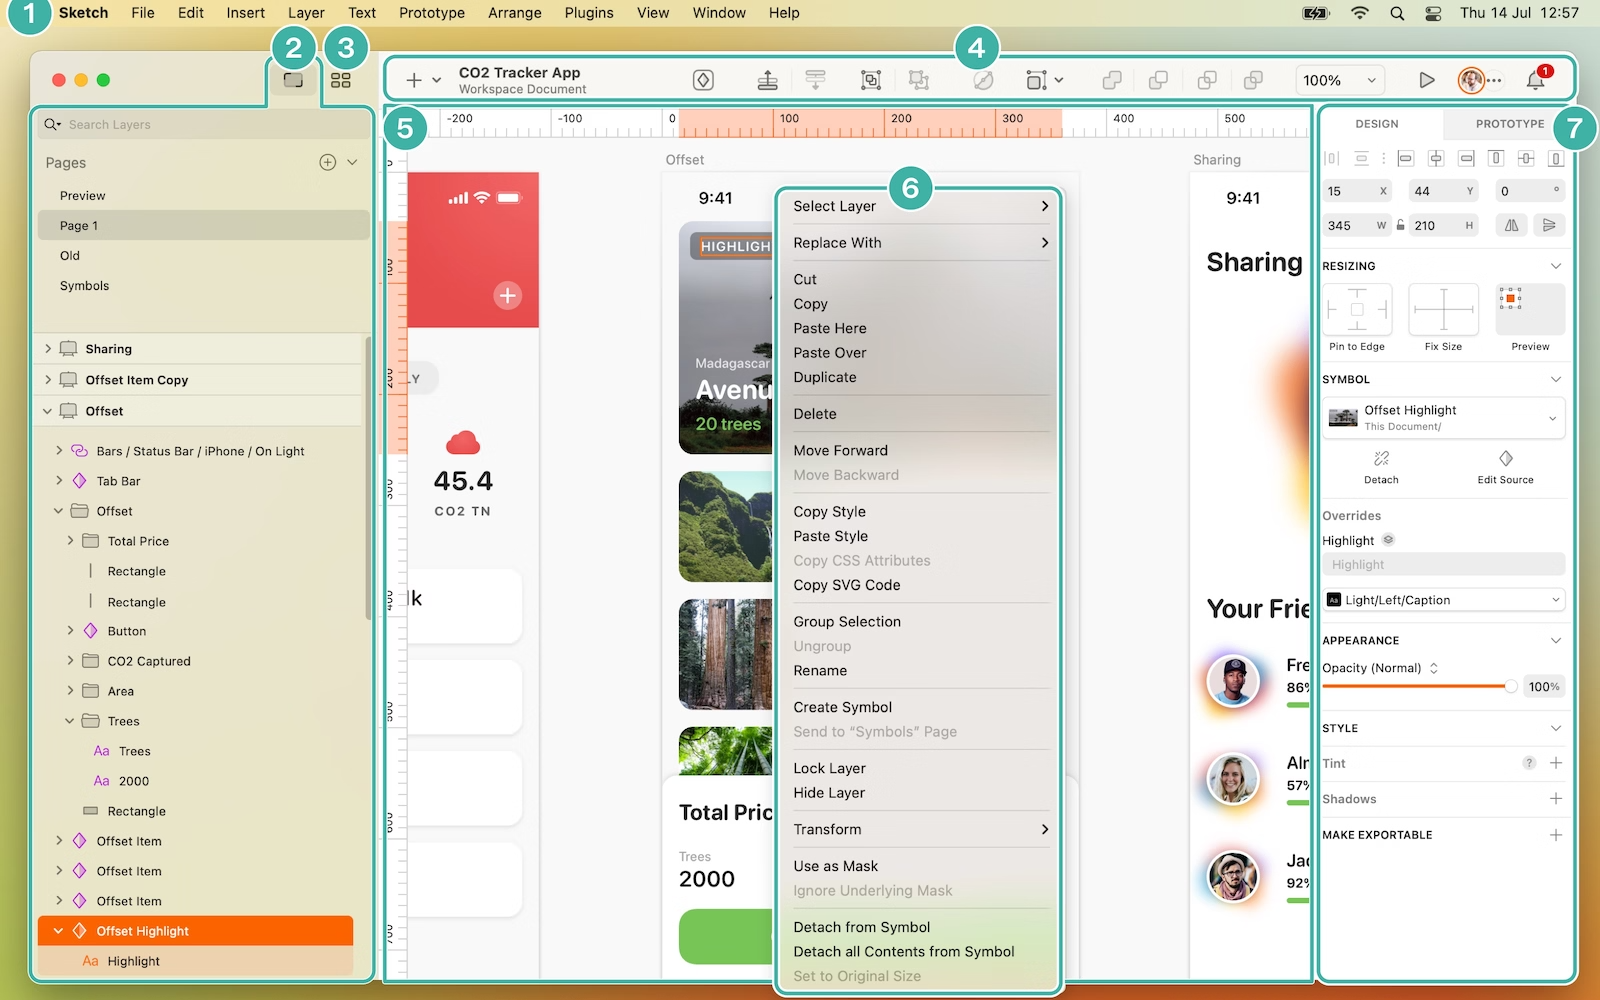
\includegraphics[width=0.8\textwidth]{\FIGDIR/sketch}
    \caption{Ukázka nástroje Sketch\cite{sketch}}
    \label{fig:sketch}
\end{figure}

%%% TODO: Podsekce - Výběr nástroje
%%% --------------------------------------------------------------
\subsection{Výběr nástroje}
\label{subsec:navrh-ui-nastroje-vyber}
Po podrobném zhodnocení byl pro návrh uživatelského rozhraní vyvíjené aplikace na prodej vstupenek s rezervací míst vybrán nástroj \textbf{Figma} z několika důvodů:

\textbf{Cloudově založený}: Figma umožňuje snadný přístup k návrhu z jakéhokoli zařízení, čímž odpadá nutnost instalace jakéhokoliv softwaru.
Nezáleží tedy ani na operačním systému, postačí pouze webový prohlížeč a připojení k internetu.

\textbf{Spolupráce v reálném čase}: I když se jedná o samostatný projekt, funkce spolupráce v reálném čase se ukazuje jako výhodná při poptávání zpětné vazby od možných budoucích zákazníků nebo konzultanta, čímž se zefektivňuje proces návrhu.

\textbf{Prototypování}: Rozsáhlé prototypovací schopnosti Figma usnadňují tvorbu interaktivních prototypů s vysokou kvalitou a důvěryhodností.

\textbf{Bezplatný}: Figma nabízí bezplatný plán, který je dostatečný pro většinu projektů.
Jedná se tedy o velmi výhodné řešení pro projekt, který není komerční či pro začínající návrháře.

\textbf{Vlastní zkušenost}: Osobně jsem měl možnost pracovat se všemi třemi nástroji a Figma se ukázala jako nejvhodnější pro tento projekt.
Zejména z důvodu jednoduchého uživatelského rozhraní, lehkosti použití a rychlosti prototypování.

%%% Sekce - Uživatelské příběhy
%%% --------------------------------------------------------------
\section{Uživatelské příběhy}
\label{sec:navrh-ui-uzivatelske-pribehy}
Při navrhování uživatelského rozhraní (\ac{ui}) nejde pouze o estetiku nebo funkčnost; vyžaduje to pochopení potřeb a očekávání uživatele.
Zahrnuje vytváření cesty, která uživatele bezproblémově provede aplikací a zároveň zajistí, aby mohli své úkoly vykonávat efektivně a s potěšením.
Technika, která se často používá v návrhu \ac{ui}/\ac{ux} k dosažení tohoto cíle, se nazývá \textit{User Stories} (uživatelské příběhy).
Uživatelské příběhy slouží jako nástroj, který pomáhá udržovat návrh zaměřený na uživatele a zajišťuje, že konečný produkt efektivně splňuje jeho potřeby.

Uživatelské příběhy, z anglického \foreign{User Stories}, jsou stručné, přímočaré popisy funkce nebo funkcionality, vyprávěné z pohledu uživatele.
Tyto příběhy kladou důraz na to, čeho uživatelé chtějí dosáhnout, podporují empatii a podporují návrhový proces, který se zaměřuje na uživatele.
Porozumění roli uživatelských příběhů při návrhu \ac{ui} webového řešení pro prodej vstupenek je klíčové pro efektivní splnění potřeb koncových uživatelů.

%%% TODO: Podsekce - Co jsou User Stories
%%% --------------------------------------------------------------
\subsection{Co jsou uživatelské příbehy}
\label{subsec:navrh-ui-uzivatelske-pribehy-co-jsou}

Uživatelské příběhy jsou součástí agilních vývojových praktik, široce používaných v návrhu \ac{ui}/\ac{ux} k zachycení zjednodušených popisů potenciálních funkcí aplikace z pohledu koncových uživatelů.
Slouží jako rychlý a jednoduchý způsob, jak popsat uživatele, co chtějí a proč to chtějí.
Každá \foreign{User Story} následuje strukturovaný formát:

\begin{gray-box}{Formát uživatelského příběhu}
    ``\textbf{Jako} [\textit{typ uživatele}] \textbf{chci} [\textit{vykonat nějakou akci}], \textbf{abych} [\textit{dosáhl nějakého cíle}].``
\end{gray-box}

V tomto formátu:
\begin{itemize}
    \item \textbf{Typ uživatele} pomáhá definovat roli uživatele, který bude používat danou funkcionalitu.
    \item \textbf{Vykonat nějakou akci} umožňuje zjistit, co chce uživatel pomocí dané funkcionality udělat nebo čeho chce dosáhnout.
    \item \textbf{Dosáhl nějakého cíle} vysvětluje základní motivaci nebo hodnotu, kterou uživatel získá provedením akce.
\end{itemize}

Tento formát je velmi užitečný při vytváření uživatelských příběhů, jelikož pomáhá udržovat stručnost, jednoznačnost a zároveň poskytuje dostatek informací, aby bylo možné pochopit, co uživatel chce a proč to chce.

Uživatelské příběhy hrají také klíčovou roli při definování akceptačních kritérií, která dále podrobně popisují, jak by měla určitá funkce fungovat z pohledu uživatele.
To pomáhá stanovit jasnou představu o účelu a očekávaném chování funkce, čímž usměrňuje její vývoj a testování.

V kontextu navrhovaného uživatelského rozhraní pro webové řešení prodeje vstupenek mohou tyto uživatelské příběhy pomoci přesně určit funkcionality, které jsou pro uživatele nejdůležitější.
Pomáhají porozumět potencionálním uživatelům –~návštěvníkům událostí, jejich potřebám (jako jsou např.\ prohlížení místa konání, výběr sedadel), jejich akce (přidání vstupenek do košíku, přechod k zaplacení) a jejich motivaci (užít si bezproblémový nákup vstupenek).

Následující sekce se zabývá tím, jak lze uživatelské příběhy konkrétně použít k navrhování uživatelského rozhraní.

%%% TODO: Podsekce - Psaní efektivních uživatelských příběhů
%%% --------------------------------------------------------------
\subsection{Psaní efektivních uživatelských příběhů}
\label{subsec:navrh-ui-uzivatelske-pribehy-psani-efektivnich}

Při psaní efektivních uživatelských příběhů pro platformu prodeje vstupenek je klíčové porozumět perspektivě koncového uživatele.
Tento proces vyžaduje identifikaci potřeb, motivací a požadovaných výsledků uživatele při používání platformy.
Některé očekávané úkoly pro platformu prodeje vstupenek mohou zahrnovat prohlížení události, výběr sedadla a dokončení nákupu vstupenky.

První krok je identifikace a pochopení různých ``personas`` nebo typů uživatelů, kteří budou pravděpodobně s platformou interagovat.
Pro platformu prodeje vstupenek je primárním uživatelem obvykle někdo, kdo má zájem o nákup vstupenek na události.
Sekundární uživatelé, jako jsou organizátoři událostí nebo manažeři prostorů, však mohou také s platformou interagovat s odlišnými požadavky na funkcionalitu.

Dalším krokem je zjištění, co uživatelé chtějí dosáhnout.
To může zahrnovat jednoduché úkoly, jako je ``prohlížení nadcházejících událostí``, nebo složitější úkoly, jako je ``rezervace místa na konkrétní událost``.
Každý uživatelský příběh by měl zůstat stručný a zaměřený na jednu akci.

Posledním krokem je definování ``hodnoty`` nebo ``výhody``, kterou uživatel získá provedením dané akce, což je známé jako jeho motivace.
Tento krok je klíčový, protože pomáhá při prioritizaci funkcí na základě hodnoty, kterou poskytují uživateli.

Při tvoření těchto uživatelských příběhů je užitečné dodržovat princip \foreign{INVEST} (\foreign{Independent}, \foreign{Negotiable}, \foreign{Valuable}, \foreign{Estimable}, \foreign{Small}, \foreign{Testable}).
Tento princip zajišťuje, že každý uživatelský příběh je dobře definován a má potřebné charakteristiky pro efektivní implementaci v procesu vývoje.

Příkladem uživatelského příběhu pro platformu prodeje vstupenek může být:

\begin{gray-box}{Ukázka uživatelského příběhu}
    \textit{``Jako zákazník si chci být schopen vybrat konkrétní sedadlo, abych se mohl akce zúčastnit.``}
\end{gray-box}

Tento uživatelský příběh je nezávislý na ostatních uživatelských příbězích, je jednoduchý a snadno pochopitelný, poskytuje hodnotu uživateli a je snadno testovatelný.
Při dodržení tohoto principu mohou uživatelské příběhy poskytnout cenný náhled do toho, jak by měla platforma prodeje vstupenek fungovat z pohledu uživatele.

%%% TODO: Podsekce - Uživatelské příběhy aplikace
%%% --------------------------------------------------------------
\subsection{Uživatelské příběhy aplikace}
\label{subsec:navrh-ui-uzivatelske-pribehy-aplikace}
Na základě pochopení získaného v předchozích sekcích se lze nyní zaměřit na konstrukci konkrétních uživatelských příběhů pro implementované webové řešení prodeje vstupenek s rezervací míst.
Nejprve je však nutné definovat hlavní uživatelský typ, který bude tuto aplikaci používat.
V základu lze říci, že hlavní rolí uživatele je potencionální zákazník, který má zájem o nákup vstupenky na konkrétní událost.
Pro další účely bude ale použito pouze záměrné označení ``zákazník``.
Každý příběh bude představen ve stanoveném formátu.
Dále budou sepsána určitá kritéria přijatelnosti, dle kterých bude jednoduše zhodnotitelné splnění příběhu.
Na závěr bude diskutováno o tom, jak daný příběh ovlivňuje návrh uživatelského rozhraní.

\begin{gray-box}{Uživatelský příběh 1 – Vizualizace místa konání}
    \textit{``Jako zákazník, chci vidět, jak vypadá místo konání, abych si mohl vybrat místo, které mi bude vyhovovat.``}
\end{gray-box}

Tento uživatelský příběh zdůrazňuje důležitost jasné a intuitivní vizualizace místa konání.
Mapa musí poskytovat přesnou reprezentaci uspořádání sedadel a nabízet dostatek detailů, aby uživatelé mohli snadno vybrat místo, které jim vyhovuje.
Pro tento příběh lze kritéria přijatelnosti definovat jako:
\begin{enumerate}
    \item Mapa místa konání je dobře viditelná
    \item Mapa místa konání přesně reprezentuje uspořádání sedadel
    \item Sedadla na mapě jsou jasně označena a snadno rozpoznatelná
\end{enumerate}

\begin{gray-box}{Uživatelský příběh 2 – Výběr sedadla}
    \textit{``Jako zákazník, si chci označit či odznačit konkrétní sedadla, abych si mohl vybrat místa, která mi budou vyhovovat.``}
\end{gray-box}

Flexibilní výběr sedadla je klíčovým prvkem prodeje vstupenek.
Uživatelé by měli mít možnost vybrat si konkrétní sedadlo, které jim vyhovuje, a měli by mít možnost si vybrat více sedadel, pokud si přejí sedět s přáteli nebo rodinou.
Uživatelské rozhraní by tedy mělo uživatelům umožnit snadno vybrat a zrušit výběr sedadel, aby mohli vyzkoušet různé možnosti výběru, které jsou k dispozici.
Pro tento příběh jsou kritéria přijatelnosti následující:
\begin{enumerate}
    \item Uživatelé mohou kliknutím vybrat konkrétní sedadlo
    \item Uživatelé mohou vybrat více sedadel
    \item Zvolená sedadla jsou jasně označena
    \item Uživatelé mohou kliknutím zrušit výběr sedadla
\end{enumerate}

\begin{gray-box}{Uživatelský příběh 3 – Nákupní košík}
    \textit{``Jako zákazník, chci mít jasný přehled o přidaných vstupenkách do nákupního košíku, abych měl přehled o svém nákupu.``}
\end{gray-box}

Tento uživatelský příběh například zdůrazňuje důležitost uživatelského rozhraní nákupního košíku se vstupenkami.
Uživatelé by měli mít možnost snadno zobrazit, jaké vstupenky mají v nákupním košíku, a měli by mít možnost snadno upravovat jeho obsah.
To vyžaduje jednoduché a přístupné uživatelské rozhraní spravující funkci nákupního košíku.
Pro přijetí tohoto příběhu jsou adekvátní kritéria přijatelnosti:
\begin{enumerate}
    \item Uživatel může snadno zobrazit aktuálně přidané vstupenky v nákupním košíku
    \item Uživatel může upravovat přidané vstupenky v košíku
    \item Uživatel může vstupenky z košíku odebrat
    \item Uživatel může zobrazit celkovou cenu nákupu
\end{enumerate}

\begin{gray-box}{Uživatelský příběh 4 – Vyřízení objednávky}
    \textit{``Jako zákazník, chci jasný a jednoduchý proces vyřízení objednávky, abych mohl svůj nákup vstupenek sebejistě dokončit.``}
\end{gray-box}

Poslední zmíněný uživatelský příběh se zaměřuje na proces vyřízení objednávky.
Zdůrazňuje potřebu jednoduchého a intuitivního uživatelského rozhraní, které umožní uživatelům snadno dokončit svůj nákup vstupenek.
Uživatelské rozhraní dokončení objednávky by tedy mělo minimalizovat komplexitu a zmatečnost, čímž zajistí uživatelům důvěru při dokončování své objednávky.
Pro tento příběh sestrojit kritéria přijatelnosti následovně:
\begin{enumerate}
    \item Proces dokončení objednávky je jednoduchý a intuitivní
    \item Objednávku lze dokončit v několika málo krocích
    \item Uživatel obdrží potvrzení o dokončení objednávky
\end{enumerate}

Z důvodu zachování přehlednosti a jednoduchosti, ačkoliv by mohlo být vytvořeno více uživatelských příběhů, budou v této práci použity pouze tyto čtyři hlavní uživatelské příběhy.
Tyto příběhy, budou v následující kapitole použity jako základní stavební kameny pro návrh uživatelského rozhraní vyvíjené webové aplikace.


%%% Sekce - Návrh UI mapy
%%% --------------------------------------------------------------
\section{Návrh UI mapy}
\label{sec:navrh-ui-mapa}
TODO: navrh rozhraní mapy, sedadel, hlavní komponenta

    %%%%% Kapitola 5 - Implementace frontendu
%%%%% ------------------------------------------------------------
\chapter{Implementace frontendu}
\label{chap:implementace-frontendu}

%%% Sekce - Analýza specifikací
%%% --------------------------------------------------------------
\section{Analýza specifikací}
\label{sec:implementace-analyza}
TODO: analýza specifikací z technického hlediska, popis problémů a možnosti jejich řešení

%%% Sekce - Výběr technologií
%%% --------------------------------------------------------------
\section{Výběr technologií}
\label{sec:implementace-vyber-technologii}
TODO: výběr technologií, popis výhod a nevýhod, základní popis

%%% Sekce - Vytvoření projektu
%%% --------------------------------------------------------------
\section{Vytvoření projektu}
\label{sec:implementace-vytvoreni-projektu}
TODO: popis postupu vytvoření projektu, co bylo použito, jak, atd.

%%% Sekce - Základní struktura projektu
%%% --------------------------------------------------------------
\subsection{Základní struktura projektu}
\label{sec:implementace-vytvoreni-projektu-zakladni-struktura}
TODO: popis základní struktury projektu, co obsahuje, jak je strukturován složkami a soubory atd.

%%% Sekce - Pomocná knihovna
%%% --------------------------------------------------------------
\subsection{Pomocná knihovna}
\label{sec:implementace-vytvoreni-projektu-pomocna-knihovna}
TODO: popis vlastní obecné pomocné knihovny, co obsahuje (utils, hooks, atd.)

%%% Sekce - Implementace nákupního košíku
%%% --------------------------------------------------------------
\section{Implementace nákupního košíku}
\label{sec:implementace-kosik}
TODO: popis implementace nákupního košíku, jeho data, správa, funkčnosti, atd.\\
TODO: další podkapitoly

%%% Sekce - Implementace mapy
%%% --------------------------------------------------------------
\section{Implementace mapy}
\label{sec:implementace-mapa}
TODO: popis implementace mapy, jaké jsou její části, jaké jsou její vlastnosti, atd.\\
TODO: další podkapitoly

%%% Sekce - Dokuemntace
%%% --------------------------------------------------------------
\section{Dokumentace}
\label{sec:implementace-dokumentace}
TODO: technická dokumentace jednotlivých komponent, jak spolu fungují, jaké jsou jejich vlastnosti, atd.

    %%%%% Závěr
%%%%% ------------------------------------------------------------
\chapter*{Závěr}
\addcontentsline{toc}{chapter}{Závěr}
\label{ch:zaver}
TODO: zhodnocení finálního prototypu oproti specifikacím, popis dalších možností vývoje, závěr

%%% seznam použité literatury
%%% Reference se hledají v souboru priklady_literatury.bib. Aby se
%%% vytvořil seznam literatury, je třeba ocitovat alespoň jednu
%%% referenci, zkompilovat tento soubor latexem, pak bibtexem a znovu
%%% latexem. Tím se vytvoří seznam použitých referencí
%%% (BcPrace.bbl) a vloží se do práce na místě, kde se nachází příkaz
%%% \bibliography, tedy sem.
    \begin{flushleft}
    \bibliography{/Users/filipditrich/University/BC_THESIS/thesis/main}
    \end{flushleft}
%%% seznam obrázků
    \listoffigures
%%% seznam tabulek
    \listoftables
%%% zkratky
    %%% TODO
%%% Použité zkratky v bakalářské práci, včetně jejich vysvětlení.
%%% --------------------------------------------------------------
\chapter*{Seznam použitých zkratek}
\addcontentsline{toc}{chapter}{Seznam použitých zkratek}
\begin{description}
    \item[API] Application Programming Interface
    \item[SVG] Scalable Vector Graphics
    \item[HTML] HyperText Markup Language
\end{description}

%%% přílohy
    %%% Přílohy k bakalářské práci, existují-li (různé dodatky jako výpisy programů,
%%% diagramy apod.). Každá příloha musí být alespoň jednou odkazována z vlastního
%%% textu práce. Přílohy se číslují.
\appendix
\addtocontents{toc}{\protect\setlength{\cftsecnumwidth}{22mm}}
\chapter*{Seznam příloh}
\addcontentsline{toc}{chapter}{Seznam příloh}
\renewcommand{\thesection}{Příloha \Alph{section}}

%%% Příloha - Návrh uživatelského rozhraní
%%%%% File preparation: ✅
%%%%% Instructions: ✅
%%% --------------------------------------------------------------
\begin{section}{Návrh uživatelského rozhraní}
    \label{appendix:ui-design}
    Návrh uživatelského rozhraní v~prostředí Figma je k nalezení v~přiloženém CD v~souboru \texttt{seating-map-figma.zip}.
    Archiv obsahuje soubor \texttt{seating-map.fig} a~jeho jednotlivé obrazovky exportované ve formátu PDF ve složce \texttt{/export}.
\end{section}
\newpage

%%% Příloha - Zdrojový kód aplikace
%%%%% File preparation: ✅
%%%%% Instructions: ✅
%%% --------------------------------------------------------------
\begin{section}{Zdrojový kód aplikace}
    \label{appendix:source-code}
    Zdrojový kód aplikace je k~nalezení v~přiloženém CD v~\texttt{seating-map-source.zip}.
    Pro spuštění aplikace je nutné mít nainstalované prostředí Node.js\footnote{\url{https://nodejs.org/en}} a nástroj pnpm\footnote{\url{https://pnpm.io/installation}}.

    Postup pro spuštění aplikace:

    \begin{enumerate}
        \item Rozbalte archiv \texttt{seating-map-source.zip}.
        \subitem \texttt{unzip seating-map-source.zip}
        \item Otevřete složku \texttt{seating-map-source} v~terminálu.
        \subitem \texttt{cd seating-map-source}
        \item Spusťte aplikaci příkazem \texttt{pnpm demo}\footnote{Příkaz nainstaluje potřebné balíčky, vytvoří potřebný \texttt{.env} soubor, sestaví aplikaci a spustí~ji lokálně na portu \texttt{3008}}.
        \subitem \texttt{pnpm demo}
        \item Aplikace bude dostupná na adrese \url{http://localhost:3008}
    \end{enumerate}

    Aplikaci je možné navštívit online na adrese \url{https://seating-map.vercel.app}.
\end{section}

\end{document}
